%%%%%%%%%%%%%%%%%%%%%%%%%%%%%%%%%%%%%%%%%%%%%%%%%%%%%%%%%%%%%%%%%%%%%%%%%%%%%%%%
%
% Template license:
% CC BY-NC-SA 3.0 (http://creativecommons.org/licenses/by-nc-sa/3.0/)
%
%%%%%%%%%%%%%%%%%%%%%%%%%%%%%%%%%%%%%%%%%%%%%%%%%%%%%%%%%%%%%%%%%%%%%%%%%%%%%%%%

%----------------------------------------------------------------------------------------
%	PACKAGES AND OTHER DOCUMENT CONFIGURATIONS
%----------------------------------------------------------------------------------------

\documentclass[
11pt, % The default document font size, options: 10pt, 11pt, 12pt
%oneside, % Two side (alternating margins) for binding by default, uncomment to switch to one side
%chapterinoneline,% Have the chapter title next to the number in one single line
spanish,
singlespacing, % Single line spacing, alternatives: onehalfspacing or doublespacing
%draft, % Uncomment to enable draft mode (no pictures, no links, overfull hboxes indicated)
%nolistspacing, % If the document is onehalfspacing or doublespacing, uncomment this to set spacing in lists to single
%liststotoc, % Uncomment to add the list of figures/tables/etc to the table of contents
%toctotoc, % Uncomment to add the main table of contents to the table of contents
parskip, % Uncomment to add space between paragraphs
%codirector, % Uncomment to add a codirector to the title page
headsepline, % Uncomment to get a line under the header
]{MastersDoctoralThesis} % The class file specifying the document structure

\usepackage{dirtree}

%----------------------------------------------------------------------------------------
%	INFORMACIÓN DE LA MEMORIA
%----------------------------------------------------------------------------------------

\thesistitle{Medición y aceptación de parámetros en transformadores de corriente alterna} % El títulos de la memoria, se usa en la carátula y se puede usar el cualquier lugar del documento con el comando \ttitle

% Nombre del posgrado, se usa en la carátula y se puede usar el cualquier lugar del documento con el comando \degreename
\posgrado{Carrera de Especialización en Sistemas Embebidos} 
%\posgrado{Carrera de Especialización en Internet de las Cosas} 
%\posgrado{Carrera de Especialización en Intelegencia Artificial}
%\posgrado{Maestría en Sistemas Embebidos} 
%\posgrado{Maestría en Internet de las cosas}

\author{Ing. Cristian Trinidad} % Tu nombre, se usa en la carátula y se puede usar el cualquier lugar del documento con el comando \authorname

\director{Esp. Lic. Leopoldo A. Zimperz (Iris Tecnologia S.R.L.)} % El nombre del director, se usa en la carátula y se puede usar el cualquier lugar del documento con el comando \dirname
\codirector{Nombre del codirector (pertenencia)} % El nombre del codirector si lo hubiera, se usa en la carátula y se puede usar el cualquier lugar del documento con el comando \codirname.  Para activar este campo se debe descomentar la opción "codirector" en el comando \documentclass, línea 23.

\juradoUNO{Mg. Ing. Gonzalo Sánchez (FAA)} % Nombre y pertenencia del un jurado se usa en la carátula y se puede usar el cualquier lugar del documento con el comando \jur1name
\juradoDOS{Mg. Ing. Gerardo Puga (UNLP)} % Nombre y pertenencia del un jurado se usa en la carátula y se puede usar el cualquier lugar del documento con el comando \jur2name
\juradoTRES{Esp. Ing. Agustín Rey (FIUBA)} % Nombre y pertenencia del un jurado se usa en la carátula y se puede usar el cualquier lugar del documento con el comando \jur3name

\ciudad{Ciudad Autónoma de Buenos Aires}
%\ciudad{ciudad de Mendoza}

\fechaINICIO{junio de 2020}
\fechaFINAL{junio de 2021}


\keywords{Sistemas embebidos, FIUBA} % Keywords for your thesis, print it elsewhere with \keywordnames


\begin{document}


\frontmatter % Use roman page numbering style (i, ii, iii, iv...) for the pre-content pages

\pagestyle{plain} % Default to the plain heading style until the thesis style is called for the body content


%----------------------------------------------------------------------------------------
%	RESUMEN - ABSTRACT 
%----------------------------------------------------------------------------------------

\begin{abstract}
\addchaptertocentry{\abstractname} % Add the abstract to the table of contents
%
%The Thesis Abstract is written here (and usually kept to just this page). The page is kept centered vertically so can expand into the blank space above the title too\ldots
\centering

La presente memoria describe el desarrollo de un prototipo encargado de medir, registrar y calificar los parámetros de transformadores de tensión alterna empleados en la fabricación de dispositivos electromédicos. Con este trabajo se busca acelerar el proceso de calificación de transformadores que actualmente se realiza manualmente por un operador. Este trabajo fue realizado para la empresa Iris Tecnología S.R.L.

Para llevar a cabo el trabajo se utilizaron algunos de los conceptos aprendidos a lo largo de la carrera como el manejo de tareas, colas y semáforos en sistemas operativos de tiempo real, acceso a un servidor web por medio de protocolos de internet como HTTP y conexiones inalámbricas, desarrollo de pruebas de aceptación y criterios generales de desarrollo circuitos impresos.

\end{abstract}

%----------------------------------------------------------------------------------------
%	CONTENIDO DE LA MEMORIA  - AGRADECIMIENTOS
%----------------------------------------------------------------------------------------

%\begin{acknowledgements}
%\addchaptertocentry{\acknowledgementname} % Descomentando esta línea se puede agregar los agradecimientos al índice
%\vspace{1.5cm}

%Esta sección es para agradecimientos personales y es totalmente \textbf{OPCIONAL}.  

%\end{acknowledgements}

%----------------------------------------------------------------------------------------
%	LISTA DE CONTENIDOS/FIGURAS/TABLAS
%----------------------------------------------------------------------------------------

\tableofcontents % Prints the main table of contents

\listoffigures % Prints the list of figures

\listoftables % Prints the list of tables


%----------------------------------------------------------------------------------------
%	CONTENIDO DE LA MEMORIA  - DEDICATORIA
%----------------------------------------------------------------------------------------

%\dedicatory{\textbf{Dedicado a... [OPCIONAL]}}  % escribir acá si se desea una dedicatoria

%----------------------------------------------------------------------------------------
%	CONTENIDO DE LA MEMORIA  - CAPÍTULOS
%----------------------------------------------------------------------------------------

\mainmatter % Begin numeric (1,2,3...) page numbering

\pagestyle{thesis} % Return the page headers back to the "thesis" style

% Incluir los capítulos como archivos separados desde la carpeta Chapters

% Chapter 1

\chapter{Introducción general} % Main chapter title

\label{Chapter1} % For referencing the chapter elsewhere, use \ref{Chapter1} 
\label{IntroGeneral}

%----------------------------------------------------------------------------------------

% Define some commands to keep the formatting separated from the content 
\newcommand{\keyword}[1]{\textbf{#1}}
\newcommand{\tabhead}[1]{\textbf{#1}}
\newcommand{\code}[1]{\texttt{#1}}
\newcommand{\file}[1]{\texttt{\bfseries#1}}
\newcommand{\option}[1]{\texttt{\itshape#1}}
\newcommand{\grados}{$^{\circ}$}

En este capítulo se presenta una introducción a los transformadores y sus ensayos de caracterización mas comunes. Asimismo, se introducen algunos equipos disponibles en el mercado y por último, se aborda el alcance y objetivo del trabajo realizado.

%----------------------------------------------------------------------------------------

%\section{Introducción}

%----------------------------------------------------------------------------------------
\section{Introducción a los transformadores}

Un transformador eléctrico es una máquina estática de corriente alterna que permite aumentar o disminuir la tensión y corriente de un circuito. La frecuencia de la onda de entrada se mantiene invariable a la salida y, en el caso de un transformador ideal, la potencia también se mantiene constante. El transformador utiliza el principio de la inducción electromagnética para su funcionamiento. En la figura \ref{fig:figTransformador} se muestra la imagen de un transformador típico de baja tension \citep{TRAFO_WIKI}, \citep{TRAFO_2}.

\begin{figure}[h]
	\centering
	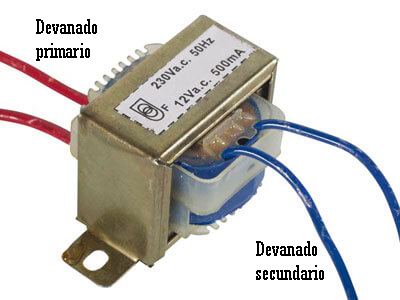
\includegraphics[scale=.5]{./Figures/transformador.jpg}
	\caption{Transformador de baja potencia\protect\footnotemark}
	\label{fig:figTransformador}
\end{figure}

\footnotetext{Imagen tomada de \url{https://www.ingmecafenix.com/electronica/transformador-electrico/}}

El transformador está constituido por dos bobinas de material conductor devanadas sobre un núcleo cerrado de material ferromagnético. Las bobinados se denominan primario y secundario según corresponda a la entrada o salida del sistema. Las bobinas o bobinados están aislados eléctricamente entre sí, la única conexión entre estos la constituye el flujo magnético que se establece en el núcleo por la circulación de corriente por dichos bobinados. Por su parte, el núcleo generalmente se fabrica de láminas apiladas de hierro o acero, de esta forma, se optimiza el flujo magnético generado por las corrientes circulantes en los bobinados. En la figura \ref{fig:figTransformador2} se muestra el principio de funcionamiento de un transformador.

\begin{figure}[htpb]
	\centering
	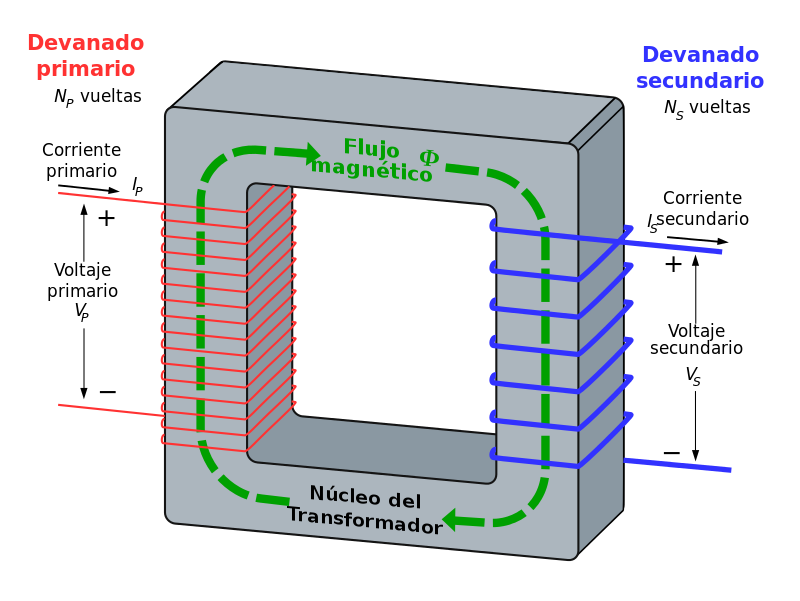
\includegraphics[scale=.3]{./Figures/transformador_2.png}
	\caption{Transformador monofásico ideal\protect\footnotemark}
	\label{fig:figTransformador2}
\end{figure}

\footnotetext{Imagen tomada de \url{https://es.wikipedia.org/wiki/Transformador}}

Existen transformadores con más de dos bobinados y diferentes arquitecturas de conexionado, un ejemplo lo constituye el transformador trifásico que está formado por 6 bobinados que pueden ser conectados en estrella o triangulo.

Actualmente, se pueden encontrar una gran variedad de transformadores para infinidad de aplicaciones, una clasificación posible es la siguiente \citep{TRAFO_APL}:

\begin{itemize}
\item Transformador de potencia.
\item Transformador de distribución.
\item Autotransformador.
\item Transformador de corriente.
\item Transformador de potencial.
\end{itemize}

Las aplicaciones van desde cargadores de teléfonos móviles hasta transformadores de potencia para estaciones y subestaciones de energía eléctrica.

\subsection{Caracterización de transformadores}

Para los cálculos de circuitos o líneas con transformadores se utiliza un circuito equivalente que representa el comportamiento del transformador real. Para la mayoría de los casos es suficiente con que dicho circuito equivalente represente el transformador en régimen permanente \citep{TRAFO_WIKI}. 

En general, se deben desarrollar diferentes ensayos sobre el transformador para determinar los parámetros de un circuito equivalente, entre los ensayos más comunes tenemos:

\begin{itemize}
\item Ensayo de vacío.
\item Ensayo de cortocircuito.
\item Ensayo de aislamiento.
\end{itemize}

En las siguientes secciones se brinda una introducción a los ensayos mencionados.

\subsubsection{Ensayo de vacío}

El ensayo de vacío es un método utilizado para determinar diversos parámetros del transformador mediante pruebas realizadas sin aplicar carga \citep{TRAFO_VACIO}. En la figura \ref{fig:figEnsayoVacio} se muestra el conexionado para este ensayo.

En este ensayo se alimenta el bobinado primario con la tensión nominal, se deja el secundario sin carga y se debe medir la tensión en los bornes del primario, la tensión en los bornes del secundario, la corriente en el devanado primario y la potencia del primario. 

\begin{figure}[htpb]
	\centering
	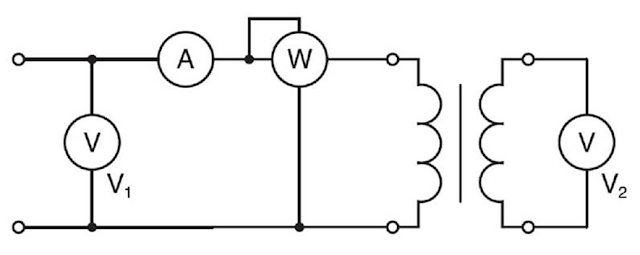
\includegraphics[scale=.4]{./Figures/EnsayoVacio.png}
	\caption{Ensayo de vació}
	\label{fig:figEnsayoVacio}
\end{figure}

\subsubsection{Ensayo de cortocircuito}
El ensayo de cortocircuito permite determinar la impedancia de cortocircuito o impedancia en serie del transformador \citep{TRAFO_CORTO}. La impedancia de cortocircuito representa las pérdidas en el cobre de los devanados, así como la inductancia de dispersión y otras inductancias parásitas. En la figura \ref{fig:figEnsayoCorto} se muestra el conexionado para este ensayo.

\begin{figure}[htpb]
	\centering
	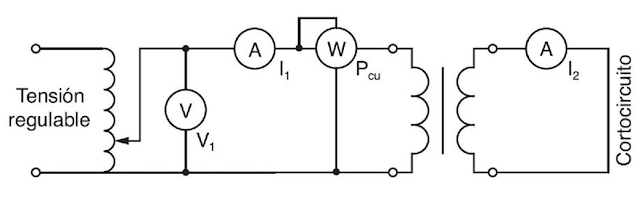
\includegraphics[scale=.5]{./Figures/EnsayoCorto.png}
	\caption{Ensayo de cortocircuito}
	\label{fig:figEnsayoCorto}
\end{figure}

En este ensayo se alimenta el bobinado primario con una tensión muy reducida, se coloca un cortocircuito en el bobinado secundario y se debe medir la tensión resultante en los bornes del primario, la corriente en el bobinado secundario, la corriente en el devanado primario y la potencia del primario. Para conseguir los valores reducidos de tensión es necesario un sistema de tensión ajustable como puede ser un autotransformador regulable. La tensión aplicada en el primario debe ser tal de hacer circular la corriente nominal por el bobinado secundario.

\subsubsection{Ensayo de aislamiento}

El ensayo de aislamiento permite determinar el estado del dieléctrico o aislante entre fases o entre una fase y el chasis del transformador \citep{TRAFO_AISL}. La medida suele dar valores en el orden de los megaohmios, valor que se ve reducido si el aislante está deteriorado.

En la figura \ref{fig:figEnsayoAislacion} se muestra un ensayo de aislamiento entre bobinas.

\begin{figure}[htpb]
	\centering
	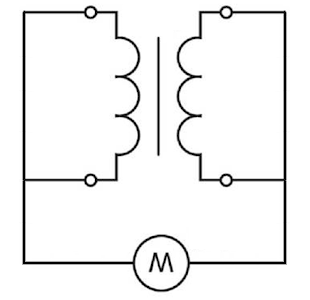
\includegraphics[scale=.5]{./Figures/EnsayoAislacion.png}
	\caption{Ensayo de aislamiento entre bobinas}
	\label{fig:figEnsayoAislacion}
\end{figure}


%----------------------------------------------------------------------------------------

\section{Estado del arte}
En la actualidad existe una variedad de equipos con el fin de caracterizar transformadores de baja tensión. Estos son capaces de caracterizar transformadores de tensión y corriente, sobre los cuales se pueden realizar múltiples ensayos y así determinar diferentes parámetros. A su vez, cuentan con interfaces de comunicación variadas como Wi-Fi, Ethernet y USB, por medio de las cuales se pueden descargar los datos medidos a una computadora para su posterior análisis. Un punto importante de estos equipos es que por lo general poseen certificaciones internaciones como por ejemplo IECs para los procedimientos de medición.

Como ejemplos podemos citar el modelo MVCT de Megger \citep{MVCT} y el modelo iCT1 de Alta Nova \citep{iCT1}. En la tabla \ref{tab:EstArte} se muestra una comparativa entre ambos equipos.

\begin{table}[htpb]
\centering
\caption[Estado del arte]{Comparación de equipos comerciales}
\resizebox{\textwidth}{!}{%
\begin{tabular}{c c c}
\hline
\toprule
\textbf{Características/Ensayos}                           & \begin{tabular}[c]{@{}c@{}}\textbf{MVCT} \\\textbf{(Megger)} \end{tabular}& \begin{tabular}[c]{@{}c@{}}\textbf{ICT1} \\\textbf{(Alta Nova)} \end{tabular}\\ \hline
Apto para transformador de corriente (TI) y tensión (TC)   & x                      & x                \\
Ensayo de relación de transformación                       & x                      & x                \\
Resistencia de bobinados                                   & x                      & x                \\
Desviación de fase                                         & x                      & x                \\
Curva de saturación (TI)                                   & x                      & x                \\
Desmagnetización (TI)                                      & x                      & x                \\
Aislamiento                                                & x                      & x                \\
Interfaz Ethernet                                          & x                      & x                \\
Interfaz Wi-Fi                                             &                        & x                \\
Interfaz USB                                               & x                      & x                \\
\bottomrule
\hline
\end{tabular}%
}
\label{tab:EstArte}
\end{table}

%----------------------------------------------------------------------------------------

\section{Motivación}
Los transformadores son una parte esencial en muchos campos de la industria, son parte fundamental en el sistema de distribución de energía, así como en equipos que son alimentados desde la red. Por esta razón, es de vital importancia su estudio y establecer métodos para conocer su estado antes de su instalación y durante su servicio.

El transformador debe estar en optimas condiciones al momento de su instalación para evitar posibles fallas del sistema donde es instalado. Un transformador cuyos parámetros esenciales están fuera de especificación puede generar un mal funcionamiento o inclusive sacar de servicio al sistema. Como ejemplo podemos citar los sistemas de distribución de energía eléctrica ya que deben ser sistemas de muy alta disponibilidad, donde un fallo en los componentes de estos sistemas puede devenir en la caída parcial o total del sistema distribución.

En el caso particular de la empresa Iris Tecnología S.R.L., que fabrica equipos electromédicos, necesita conocer si los transformadores provistos son aptos para ser utilizados en sus equipos. Para ello, la empresa cuenta con sistema de gestión de calidad basado en la norma ISO13485:2016.

Entre las tareas y controles necesarios para el sistema de gestión de la calidad se encuentra el ensayo y calificación de transformadores. Actualmente, esta tarea es realiza manualmente por un operador. Esta labor, además de insumir una gran cantidad de tiempo y ser muy repetitiva, presenta un gran riesgo de error humano y puede comprometer la seguridad del operario y la fiabilidad de los datos obtenidos.

La posibilidad de contar con un equipamiento que, con una mínima intervención del operador, pueda desarrollar los ensayos requeridos representa una gran ventaja para la empresa.

%----------------------------------------------------------------------------------------

\section{Objetivos y alcance}

\subsection{Objetivos del trabajo}

El objetivo de este trabajo fue el desarrollo de un prototipo de hardware y software que permite automatizar el proceso de caracterización de transformadores de baja tensión utilizado. El prototipo desarrollado es casi autónomo, es decir, solo requiere una mínima intervención del operador para funcionar. Por otro lado, los resultados de la caracterización son enviados a un servidor web proporcionado por el cliente, mostrados en un \textit{display} local e impresos en una etiqueta.

\subsection{Alcance del trabajo}
El presente trabajo tiene como alcance:
\begin{itemize}
\item El análisis, investigación y elección del hardware.
\item La investigación del modelo de impresora a adquirir, cuyo protocolo debe estar disponible.
\item El diseño e implementación del firmware del sistema en lenguaje C sobre FreeRTOS.
\item El desarrollo de un prototipo funcional sobre un circuito impreso universal.
\end{itemize}

Queda excluido del alcance de este trabajo:
\begin{itemize}
\item El desarrollo de circuitos de medición de tensión y/o corriente alterna de precisión. Se acepta la precisión obtenida de módulos comerciales como el ZMPT101B.
\item El desarrollo de fuentes de tensión alterna de precisión para alimentar los transformadores en ensayo.
\item El desarrollo de una aplicación web desde la cual interactuar por Wi-Fi con el módulo.
\item El desarrollo del servidor web o API de colección de datos.
\item El desarrollo de un prototipo de fabricación escalable que cumpla con todas las certificaciones necesarias.
\item El desarrollo de un circuito impreso, más allá del prototipo en placa universal.
\item El diseño de circuitos de protección del operario contra descargas eléctricas de alta tensión. En este sentido, se asume que el operario que utilizará el dispositivo es idóneo en el tema. Asimismo, se asume que el cliente posee en sus instalaciones las medidas de seguridad pertinentes para el trabajo con altas tensiones, como disyuntores y puestas a tierras, acorde con la normativa vigente de Higiene y Seguridad en el Trabajo.
\end{itemize}

\chapter{Introducción específica} % Main chapter title
\label{Chapter2}

%----------------------------------------------------------------------------------------
%	SECTION 1
%----------------------------------------------------------------------------------------
En este capítulo se presentan una introducción al trabajo realizado así como los requerimientos del sistema que fueron oportunamente consensuados con el cliente. Posteriormente, se realiza una descripción de las tecnologías utilizadas.

\section{Estructura general del sistema}

En la figura \ref{fig:diagBloques} se muestra el diagrama en bloques simplificado del sistema. En la figura se observa el dispositivo diseñado, el cual se encuentra dentro de un recuadro, y el transformador a ensayar. Dentro del dispositivo diseñado se observan los siguientes bloques principales:

\begin{itemize}
\item Módulo ESP32 con Wi-Fi integrado.
\item Bloques de acondicionamiento de señal y actuación para el bobinado primario y secundario.
\item Interfaz de usuario: pulsadores, \textit{display} y \textit{buzzer}.
\item Interfaz serie para impresora.
\item \textit{Switch} de seguridad. Se utiliza para indicar que la tapa de seguridad ha sido removida y el operario puede quedar expuesto a altas tensiones.
\item Fuente de alimentación.
\end{itemize}

El trabajo desarrollado tiene como fin determinar si un transformador dado es apto o no para ser utilizado en determinados equipos. Para tal fin, se configuran umbrales de comparación por medio de una comunicación HTTP a un servidor web y se procede a compararlos contra mediciones realizadas sobre el transformador. Una vez realizadas las comparaciones, los resultados del ensayo se muestran localmente por medio de un \textit{display}. Adicionalmente, los resultados y las mediciones realizadas son enviadas al servidor web del cliente utilizando el protocolo HTTP. Por otro lado, se cuenta con una impresora la cual imprime una etiqueta que permite la trazabilidad del transformador.

Todo el dispositivo es controlado por solo tres pulsadores: Testear, Configurar y Cancelar.

A continuación se detalla un resumen de las tareas realizadas en este trabajo:
\begin{itemize}
\item Mediciones de tensión y corriente a los transformadores bajo ensayo.
\item Pedido de umbrales de aceptación a un servidor web.
\item Emisión de aceptación o rechazo del transformador.
\item Visualización en el \textit{display} de los umbrales configurados y las mediciones realizadas.
\item Envío de las mediciones a un servidor web por medio del protocolo HTTP.
\item Gestión de la conexión Wi-Fi.
\item Impresión de etiquetas. 
\end{itemize}

\begin{figure}[htpb]
\centering 
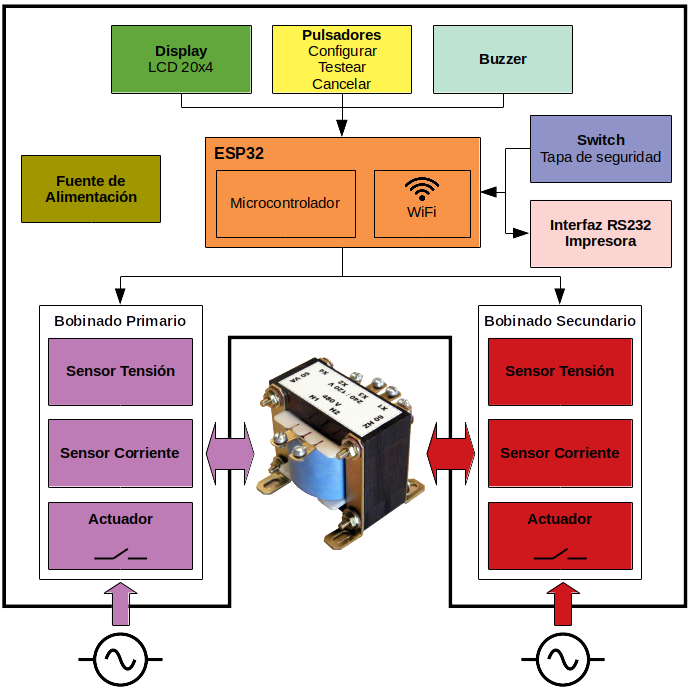
\includegraphics[width=.8\textwidth]{./Figures/diagBloques.png}
\caption{Diagrama en bloques del sistema.}
\label{fig:diagBloques}
\end{figure}


En la figura \ref{fig:FSMSimplificada} se presenta un diagrama de secuencia simplificado del dispositivo cuyos estados se describen a continuación:

\begin{figure}[htpb]
\centering 
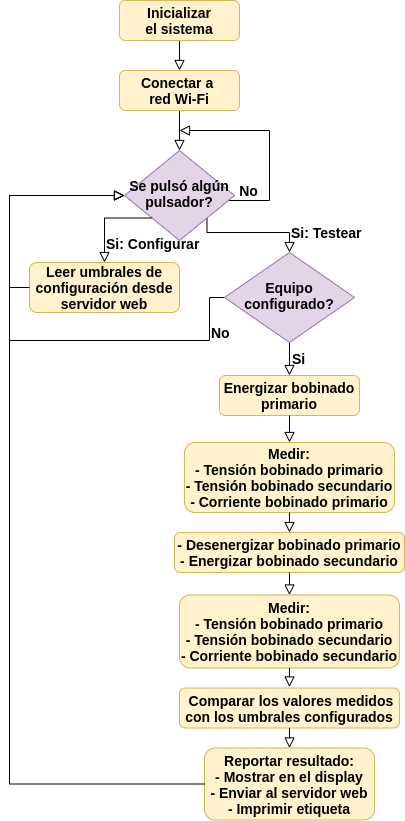
\includegraphics[width=.8\textwidth]{./Figures/FSMSimplificada.png}
\caption{Diagrama de secuencia simplificado.}
\label{fig:FSMSimplificada}
\end{figure}

\begin{enumerate}
\item Inicialización del sistema.
\item Conexión a red Wi-Fi.
\item Espera por pulsadores. El operador debe pulsar Configurar para leer los umbrales de configuración desde el servidor web.
\item Luego el operador debe pulsar Testear para iniciar la caracterización del transformador. Aquí se verifica que el equipo haya sido configurado previamente ya que no se puede caracterizar un transformador si no cuenta con los umbrales de comparación. En caso de estar configurado se procede a los siguientes pasos.
\item Energizar el bobinado primario con 230 V$_{RMS}$ estabilizados (provistos externamente por el cliente).
\item Medir:
\begin{itemize}
	\item Tensión en bobinado primario.
	\item Corriente que circula por el bobinado primario.
	\item Tensión en bobinado secundario.
\end{itemize}
\item Desenergizar el bobinado primario.
\item Energizar el bobinado secundario con la tensión adecuada. Esta tensión se genera internamente a partir de la tensión de 230 V$_{RMS}$.
\item Medir:
\begin{itemize}
	\item Tensión en bobinado primario.
	\item Tensión en bobinado secundario.
	\item Corriente que circula por el bobinado secundario.
\end{itemize}
\item Desenergizar el bobinado secundario.
\item Comparar los valores medidos con los umbrales configurados previamente y determinar si el transformador es aceptado o rechazado.
\item Reportar los valores medidos y los resultados obtenidos al:
\begin{itemize}
	\item Servidor web.
	\item En el \textit{display} local.
	\item Imprimir una etiqueta.
\end{itemize}
\end{enumerate}


\section{Requerimientos}

A continuación se enumeran los requerimientos consensuados con el cliente:

\subsection{Requerimientos de hardware}
	\begin{enumerate}
	\item El dispositivo debe ser diseñado en base al módulo ESP32.
	\item El dispositivo debe ser capaz de medir tensiones y corrientes alternas de manera aislada del transformador bajo ensayo.
	\item El dispositivo debe ser capaz de conmutar las tensiones primarias y secundarias.
	\item El dispositivo debe tener un \textit{display} LCD alfanumérico de 20x4 caracteres.
	\item El dispositivo debe tener una interfaz Wi-Fi.
	\item El dispositivo debe tener una interfaz RS-232 capaz de manejar impresoras series.
	\item El dispositivo debe alimentarse desde la red eléctrica Argentina 220 V$_{RMS}$/50 hz, debiendo proveerse todas las alimentaciones a los diferentes módulos de hardware.
	\item El dispositivo debe poseer un \textit{switch} para indicar que la tapa de seguridad ha sido removida.
	\item El dispositivo debe poseer tres pulsadores nombrados Configurar, Testear y Cancelar.
	\item El dispositivo debe poseer un \textit{buzzer}.
	\end{enumerate}
\subsection{Requerimientos relativos a los valores a medir}
	\begin{enumerate}
	\item Bobinado primario:
		\begin{enumerate}
		\item Rango tensión: 100 – 240 V$_{RMS}$.
		\item Rango corriente: 0 – 800 mA$_{RMS}$.
		\end{enumerate}
	\item Bobinado secundario:
		\begin{enumerate}
		\item Rango tensión: 0 – 30 V$_{RMS}$.
		\item Rango corriente: 0 – 1500 mA$_{RMS}$.
		\end{enumerate}
	\item Precisión en la medición de tensión: mejor al 1,5\% (puede variar en base a lo que se pueda conseguir en el mercado).
	\item Precisión en la medición de corriente: mejor al 4\% (puede variar en base a lo que se pueda conseguir en el mercado).
	\end{enumerate}
\subsection{Requerimientos funcionales}
\label{subsec:ReqFun}
	\begin{enumerate}
	\item El dispositivo debe permitir que se configuren los umbrales mínimos y máximos para los parámetros medidos. 
	\item Los valores a configurar deben ser adquiridos solo por Wi-Fi, no se admite configuración local por teclado.
	\item El dispositivo debe generar una confirmación de aceptación o rechazo del transformador en ensayo basado en los umbrales mínimos y máximos preseteados.
	\item El dispositivo luego de cada ensayo, independientemente del resultado, debe imprimir una etiqueta con la siguiente información:
		\begin{enumerate}
		\item Número de partida del transformador ensayado.
		\item Condición de aceptado o rechazado.
		\item Valores medidos de tensiones y corrientes.
		\end{enumerate}
	\end{enumerate}	
\subsection{Requerimientos de comunicación}
\label{subsec:ReqCom}
	\begin{enumerate}
	\item Solicitar parámetros de configuración: el dispositivo debe generar un comando GET de HTTP a un servidor web (provisto por el cliente) para obtener los umbrales de aceptación y el número de partida del transformador a ensayar.
	\item El dispositivo debe ser capaz de procesar la respuesta del comando GET que está en formato JSON.
	\item Enviar resultados del ensayo: el dispositivo debe generar un comando POST de HTTP a un servidor (provisto por el cliente) con la información del transformador ensayado en formato JSON.
	\end{enumerate}
\subsection{Requerimientos de interfaz de usuario}
\label{subsec:ReqUsu}
	\begin{enumerate}
	\item Sobre la funcionalidad de los pulsadores:
		\begin{enumerate}
		\item Configurar: al pulsar este pulsador el dispositivo debe generar el comando GET para solicitar al servidor web los parámetros de configuración del dispositivo a través de Wi-Fi.
		\item Testear: al pulsar este pulsador el dispositivo debe iniciar la secuencia de testeo.
		\item Cancelar: al pulsar este pulsador la secuencia de testeo en curso debe quedar abortada.
		\end{enumerate}
	\item Sobre la funcionalidad del \textit{display} LCD:
		\begin{enumerate}
		\item El dispositivo debe mostrar los umbrales configurados y los valores de las mediciones actuales.
		\item Los valores de los umbrales configurados deberán permanecer en el \textit{display} durante el ensayo.
		\item El dispositivo debe mostrar los valores medidos del transformador ensayado luego de cada medición.
		\item Luego de finalizado el ensayo se debe mostrar un mensaje que indique que la información se ha enviado al servidor web y mantenerse el dispositivo bloqueado hasta que se haya recibido la respuesta del servidor.
		\end{enumerate}
	\item Sobre el \textit{buzzer}:
		\begin{enumerate}
		\item El dispositivo debe emitir un solo sonido de 0,5 segundos de duración para confirmar la aceptación del transformador.
		\item El dispositivo debe emitir un sonido de repetición de 5 ciclos de 0,5 segundos de duración con pausas de 0,5 segundos para confirmar el rechazo del transformador.
		\end{enumerate}		
	\end{enumerate}


\section{Kit ESP32-DevKitC}

Para este trabajo se utilizó el kit de desarrollo ESP32-DevKitC \citep{ESP32} desarrollado por la empresa Espressif Systems, figura \ref{fig:ESP32DevKitC}. Este kit integra un módulo ESP32-WROOM-32 \citep{WROOM} de la misma empresa, figura \ref{fig:ESP32WROOM}. El módulo ESP32-WROOM-32 es un microcontrolador de doble núcleo con interfaces Wi-Fi y Bluetooth. Además de las interfaces anteriores, el módulo cuenta con interfaces UART, SPI, numerosas entradas-salidas de propósito general, conversores analógico-digital y conversores digital-analógico.

\begin{figure}[htpb]
	\centering
	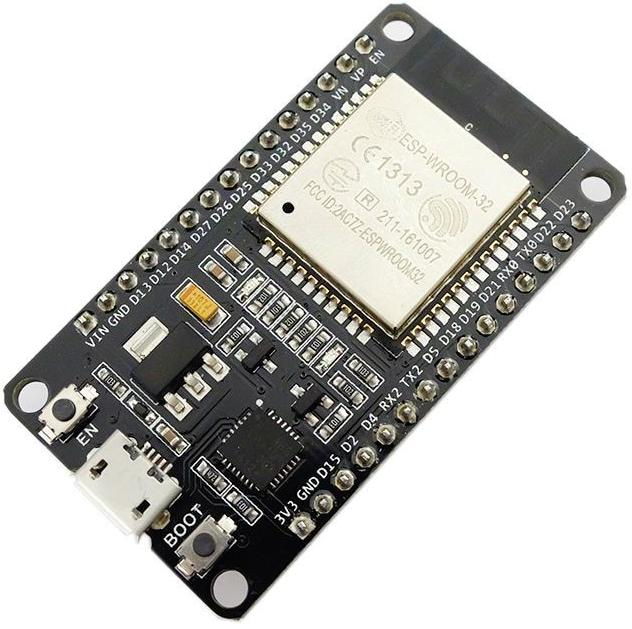
\includegraphics[scale=1.2]{./Figures/ESP32DevKit.jpg}
	\caption{ESP32-DevKitC V1.}
	\label{fig:ESP32DevKitC}
\end{figure}

\begin{figure}[htpb]
	\centering
	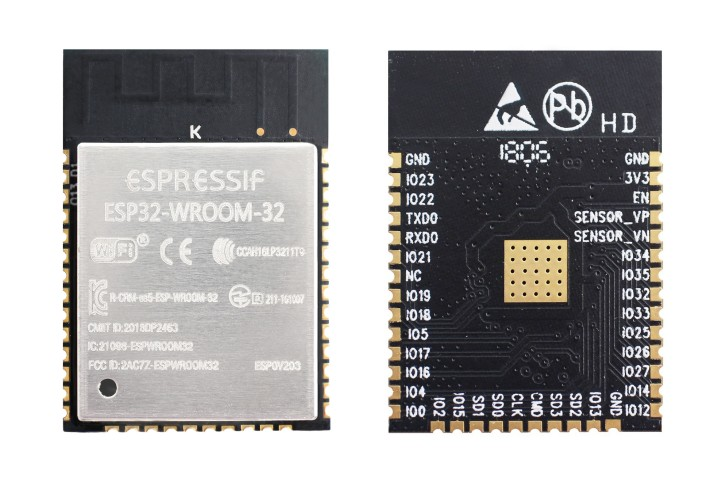
\includegraphics[scale=.5]{./Figures/esp32-wroom-32-front-back.jpg}
	\caption{ESP32-WROOM-32.}
	\label{fig:ESP32WROOM}
\end{figure}

De las especificaciones del módulo ESP32-WROOM-32 se pueden destacar las siguientes:
\begin{itemize}
\item Procesador dual core Xtensa® LX6 de 32 bits.
\item Velocidad de reloj de hasta 240 Mhz.
\item 520 KB de RAM.
\item 4 MB SPI flash.
\item Wi-Fi integrado con posibilidad de trabajar como AP (\textit{Access Point}) y SM (\textit{Station Mode}).
\item Bluetooth V4.2.
\item 36 GPIO.
\item Hasta 18 conversores anologico-digital (ADC) de 12 bits de resolución.
\item 2 conversores digital-analógico (DAC) de 8 bits de resolución.
\item 3 UART.
\item 2 canales I2C.
\item 4 canales SPI.
\item Interfaz JTAG.
\end{itemize}

Dado que el ESP32-DevKitC integra al módulo ESP32-WROOM-32, puede que no todos sus periféricos y entradas-salidas de propósito general (GPIO por sus siglas en inglés) estén disponibles. 

A continuación se detallan las principales características del kit ESP32-DevKitC:
\begin{itemize}
\item Doble hilera de pines con casi todas las entradas-salidas de propósito general del ESP32-WROOM-32.
\item Puente USB-UART conectado al módulo ESP32-WROOM-32. Esta interfaz es muy útil para programación y depuración.
\item Regulador LDO para proveer alimentación a los elementos del kit. 
\end{itemize}

\subsection{Entorno de desarrollo ESP-IDF}
\label{sec:ESPIDF}
%https://docs.espressif.com/projects/esp-idf/en/latest/esp32/about.html#:~:text=The\%20ESP\%2DIDF\%2C\%20Espressif\%20IoT,and\%20Mac\%20OS\%20operating\%20systems.

Espressif Systems provee un entorno de desarrollo de software denominado ESP-IDF \citep{ESPIDF}. El entorno ESP-IDF contiene todo lo necesario para desarrollar aplicaciones para los módulos ESP-32 sobre cualquier sistema operativo: Windows, Linux o MAC OS. Este entorno de desarrollo es \textit{Open-Source} y puede ser clonado desde un repositorio de GitHub\footnote{Repositorio GitHub para el ESP-IDF \url{https://docs.platformio.org/en/latest/frameworks/espidf.html}}. La empresa constantemente realiza actualizaciones y correcciones de fallas.

A continuación se listan algunas de las características más destacables del entorno ESP-IDF:

\begin{itemize}
\item Soporta \textit{FreeRTOS} \citep{ESPIDF:FreeRTOS}.
\item Soporta diferentes controladores de periféricos (SPI, I2C, UART, GPIO, I2S, ADC, DAC, etc) \citep{ESPIDF:PER}.
\item Soporta librerías para Wi-Fi \citep{ESPIDF:WiFi} y Bluetooth \citep{ESPIDF:bluetooth}.
\item Soporta varios \textit{stacks} de redes, por ejemplo TCP/IP.
\item Soporta varias implementaciones de protocolos (DHCP cliente y servidor, HTTP cliente y servidor, MQTT, etc) \citep{ESPIDF:PRO}.
\item Soporta extensiones para Eclipse \citep{ESPIDF:ECLIPSE} y Visual Code \citep{ESPIDF:VC}.
\item Está basado en CMake \citep{ESPIDF:CMake}.
\end{itemize}

El entorno ESP-IDF no es parte del proyecto del usuario sino que debe ser enlazado por medio de la variable de entorno IDF\_PATH. Esto último ayuda a separar el entorno de desarrollo del proyecto particular del usuario. Para utilizar ESP-IDF se requiere una estructura particular de archivos y carpetas para el proyecto \citep{ESPIDF:CMake_2}. 

\subsection{ESP-Touch y SmartConfig}
\label{sec:ESPTouch}

Espressif Systems provee la aplicación móvil ESP-Touch \citep{ESPTOUCH} la cual puede ser usada con la librería SmartConfig \citep{SMARTCONFIG} para configurar las credenciales de Wi-Fi en equipos que no posean una interfaz de usuario acorde para insertar esta información. En la figura \ref{fig:EspTouch} se muestra la interfaz de la aplicación ESP-Touch.

\begin{figure}[htpb]
	\centering
	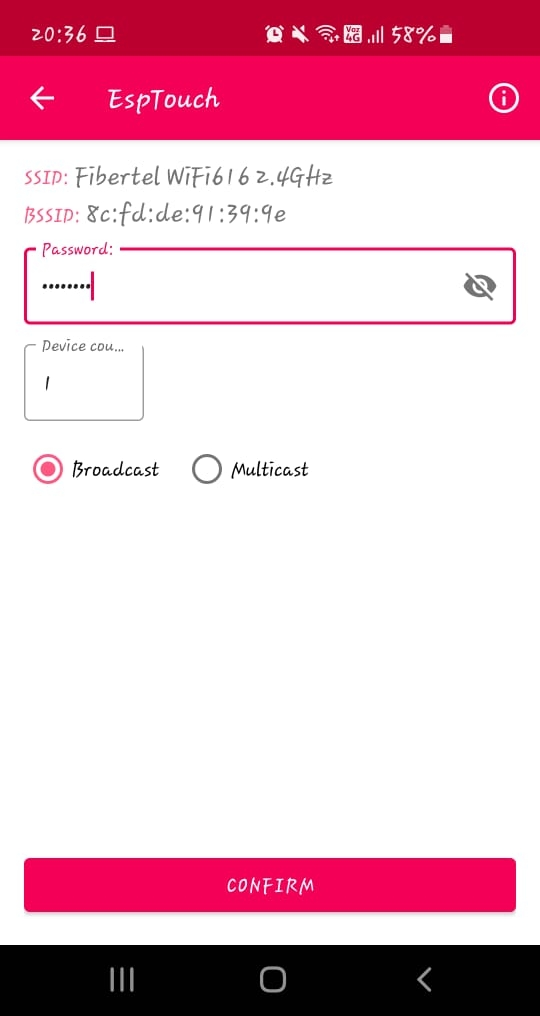
\includegraphics[scale=.5]{./Figures/EspTouch.jpeg}
	\caption{Aplicación Android ESP-Touch.}
	\label{fig:EspTouch}
\end{figure}

La ventaja de esta tecnología es que el dispositivo no necesita conocer directamente el SSID o la contraseña de un punto de acceso (AP), en cambio esta información se proporciona mediante el teléfono móvil. ESP-Touch está disponible para Android e iOS.

\section{Sensor de tensión}
\label{sec:secZMPT101B}

Para monitorear las tensiones del bobinado primario y secundario se utilizó el módulo de figura \ref{fig:ZMPT101B}.

\begin{figure}[htpb]
	\centering
	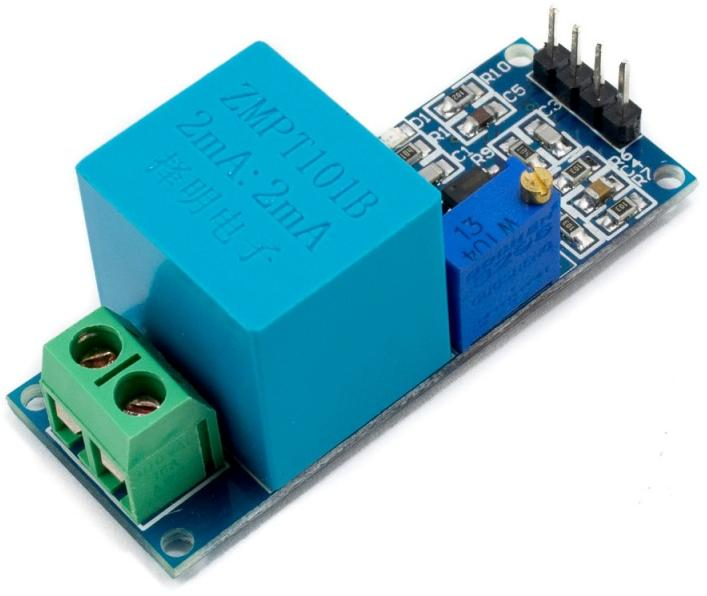
\includegraphics[scale=.3]{./Figures/zmpt101b.jpg}
	\caption{Módulo sensor de tensión alterna.}
	\label{fig:ZMPT101B}
\end{figure}

Este módulo es un sensor de tensión capaz de medir tensiones alternas de línea de 220 V$_{RMS}$ de forma aislada. En la figura \ref{fig:ZMPT101B_waves} se puede observar la tensión de entrada (Vin) y la tensión de salida (Vout) entregada por el módulo. El módulo provee una tensión de salida la cual está montada sobre un nivel continua igual a la mitad de la tensión de alimentación, esto ayuda a procesar la señal directamente con un ADC sin la necesidad de fuentes de alimentación negativas.

\begin{figure}[htpb]
	\centering
	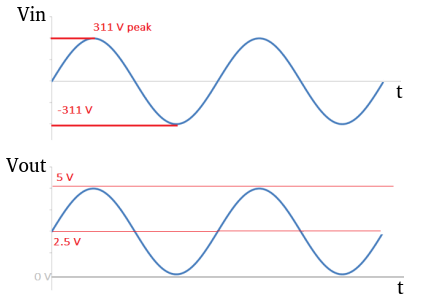
\includegraphics[scale=1.2]{./Figures/ZMPT101B_waves.png}
	\caption{Ondas de entrada (Vin) y salida (Vout) del módulo @ Vcc = 5 V.}
	\label{fig:ZMPT101B_waves}
\end{figure}

El elemento principal del módulo es el transformador de corriente ZMPT101B de la empresa Qingxian Zeming Langxi Electronic \citep{ZMPT101B_b}. Este componente es el encargado de proporcionar la aislación entre la alta tensión de línea y la baja tensión hacia el microcontrolador. El primario del transformador se conecta a la tensión alterna de la red a través de la bornera verde que se observa en la figura \ref{fig:ZMPT101B}. En el lado secundario del transformador se tiene una resistencia serie (\textit{shunt}) y un circuito amplificador basado en el operacional LM358 \citep{LM358}. Adicionalmente, el circuito posee un potenciómetro para ajustar la ganancia del sistema.

Este módulo se utiliza en aplicaciones de domótica e IoT (Internet of Things) para el monitoreo de la tensión de línea.

Especificaciones técnicas del módulo: 
\begin{itemize}
\item Tensión de alimentación (Vcc): 5-30 V.
\item Tensión alterna de entrada máxima: 250 V$_{RMS}$.
\item Tensión de salida: onda senoidal 2,5 V$_{PICO}$ @ Vcc = 5 V.
\item Valor medio de la tensión salida: 2,5 V @ Vcc = 5 V.
\item Dimensiones: 5 cm x 2 cm x 2,4 cm.
\end{itemize}

\section{Sensor de corriente}
\label{sec:secZMCT103C}

Para monitorear las corrientes del bobinado primario y secundario se utilizó el módulo de figura \ref{fig:ZMCT103C}.

\begin{figure}[htpb]
	\centering
	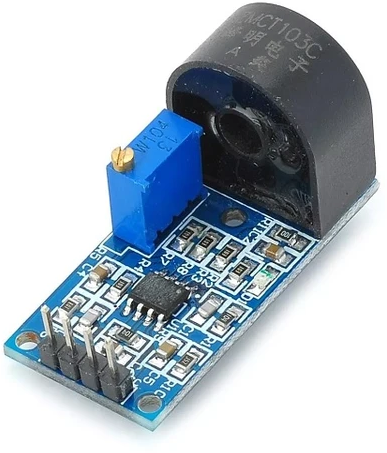
\includegraphics[scale=.5]{./Figures/ZMCT103C.png}
	\caption{Módulo sensor de corriente alterna.}
	\label{fig:ZMCT103C}
\end{figure}

Este módulo facilita el monitoreo de corriente alternas de hasta 5 A$_{RMS}$. Está basado en el transformador de corriente de alta precisión ZMCT103C de la empresa Qingxian Zeming Langxi Electronic \citep{ZMCT103C_b}. El módulo es similar al módulo sensor de tensión presentado en la sección \ref{sec:secZMPT101B}. La corriente de salida del transformador de corriente pasa por una resistencia serie (\textit{shunt}) y luego es acondicionada por los amplificadores operaciones integrados en el LM358 \citep{LM358}. La única diferencia entre el módulo sensor de corriente y el de tensión es que el primero entrega una tensión alterna con valor medio cero, es decir, sin componente de continua. Esto último hace necesario alguna modificación adicional del módulo para entregar una tensión que sea siempre positiva.

Especificaciones técnicas del módulo: 
\begin{itemize}
\item Tensión de alimentación (Vcc): 5-30 V.
\item Corriente de entrada nominal: 5 A$_{RMS}$.
\item Tensión de salida: onda senoidal 2.5 V$_{PICO}$ @ Vcc = 5 V.
\item Valor medio de la tensión salida: 0 V @ Vcc = 5 V.
\end{itemize}

\section{Impresora}
\label{sec:Impre}
Para este trabajo se utilizó una impresora de transferencia térmica modelo E-Class™ Mark III fabricada por Honeywell \citep{printer_b}, ver figura \ref{fig:printer}. Las impresoras por transferencia térmica utilizan una cinta de tinta denominada \textit{Ribbon} que con el calor del cabezal derrite la tinta sobre el papel. Este fenómeno permite imprimir códigos de barras, textos, etc. Estas impresoras son de bajo costo pero ofrecen como desventaja que solo imprimen en blanco y negro.

\begin{figure}[htpb]
	\centering
	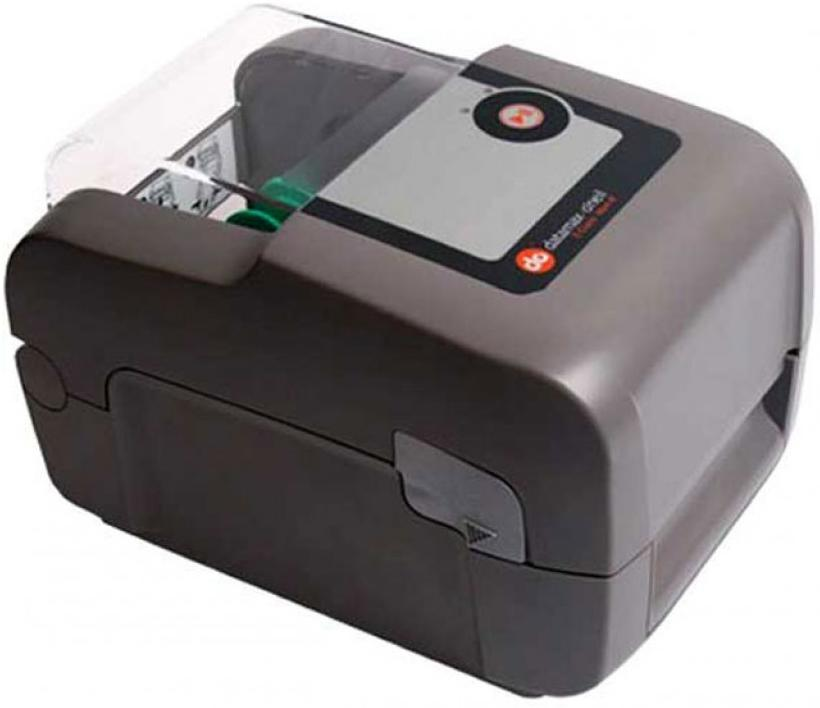
\includegraphics[scale=0.3]{./Figures/printer.jpeg}
	\caption{Impresora E-Class™ Mark III modelo E-4204B.}
	\label{fig:printer}
\end{figure}


Especificaciones técnicas del modelo E-4204B:
\begin{itemize}
\item Resolución: 8 puntos/mm (203 ppp).
\item Velocidad máxima de impresión: 101 mm/s (4 pps).
\item Ancho máximo de papel: 112 mm.
\item Capacidad de rollo: diámetro externo 127 mm.
\item Memoria: DRAM de 16 MB/Flash de 8 MB.
\item Comunicación: USB 2.0 y RS-232 serie.
\item Lenguajes soportados: DPL(Datamax), ZPL(Zebra), EPL(Eltron), BPL(Boca), IPL(Intermec).
\item Indicadores de estado: dos indicadores luminosos de tres colores.
\item Dimensiones: 187 mm x 203,5 mm x 282 mm.
\item Peso: 2,4 Kg.
\end{itemize}

\subsection{Protocolo DPL}
\label{subsec:ProDPL}
El protocolo DPL (Datamax-O’Neil \textit{Programming Language}) es un protocolo propietario de la firma Datamax el cual puede ser utilizado para comunicarse con las impresoras E-Class™ Mark III \citep{DPL_man}. Este es un protocolo punto a punto de tipo ASCII basado en la arquitectura maestro/esclavo. La impresora se conecta con el \textit{host} sin intermediarios.

El protocolo está formado por comandos y parámetros asociados a estos comandos. En la tabla \ref{tab:printercmd} se muestran los comandos disponibles.

\begin{table}[htpb]
\centering
\caption[Comandos protocolo DPL]{Tipos de comandos protocolo DPL.}
\resizebox{\textwidth}{!}{%
\begin{tabular}{c c c}
\hline
\toprule
\textbf{ASCII (HEX)} & \textbf{Tipo}     & \textbf{Descripción}\\
\midrule
SOH (0x01)  & Comando inmediato          & \begin{tabular}[c]{@{}c@{}}Cuando la impresora recibe un comando inmediato \\interrumpe su operación actual y pasa a ejecutarlo. \\Ejemplos: reinicio de la impresora, \\pedido de estado de la impresora.\end{tabular}                         \\ \hline
STX (0x02)  & Comando de sistema          & \begin{tabular}[c]{@{}c@{}}Es el tipo de comando más comúnmente utilizado. \\Ejemplos: configurar el modo de trabajo métrico o \\imperial, tipo de alineación del texto a imprimir, indica el \\inicio y fin del texto a imprimir, etc.\end{tabular} \\ \hline
ESC (0x1B)  & \begin{tabular}[c]{@{}c@{}}Comando de carga de\\fuente \end{tabular}& \begin{tabular}[c]{@{}c@{}}Este comando es utilizado para cargar una nueva fuente. \\Generalmente es utilizado por programas\\ específicos para la creación de fuentes.\end{tabular}\\ 
\bottomrule
\hline
\end{tabular}%
}
\label{tab:printercmd}
\end{table}

En las siguientes secciones se describen los comandos inmediatos y los comandos de sistema ya que fueron los utilizados en este trabajo.

\subsubsection{Comandos inmediatos}
\label{subsubsec:ProDPLCMDIn}
En la tabla \ref{tab:printercmdInmediatos} se muestran los comandos inmediatos más utilizados, en la última columna se muestra la respuesta de la impresora.

\begin{table}[htpb]
\centering
\caption[Comandos inmediatos protocolo DPL]{Comandos inmediatos protocolo DPL.}
\resizebox{\textwidth}{!}{%
\begin{tabular}{c c l}
\toprule
\textbf{ASCII (HEX)} & \textbf{Descripción} & \multicolumn{1}{c}{\textbf{Respuesta}}\\ 
\midrule
\begin{tabular}[c]{@{}c@{}}\textless{}SOH\textgreater{}A\textless{}CR\textgreater\\ (0x01,0x41,0x0D)\end{tabular} & \begin{tabular}[c]{@{}c@{}}Pedido de estado de la impresora.\end{tabular} & \begin{tabular}[c]{@{}l@{}}La respuesta son 8 caracteres 'Y' o 'N' \\mas el carácter \textless{}CR\textgreater{} de final de mensaje.\\ \\ abcdefgh\textless{}CR\textgreater\\ a: Interprete de comandos ocupado\\ b: Falla de papel\\ c: Falla del \textit{Ribbon}\\ d: Imprimiendo lote (se pueden enviar \\varias etiquetas para imprimir)\\ e: Impresora ocupada\\ f: Impresora pausada\\ g: Etiqueta presentada\\ h: Falla interna\end{tabular} \\
\begin{tabular}[c]{@{}c@{}}\textless{}SOH\textgreater{}*\textless{}CR\textgreater\\ (0x01,0x2A,0x0D)\end{tabular} & Pedido de reinicio de la impresora                                                                                                                                       & \textless{}XON\textgreater{}R\textless{}CR\textgreater{} \\ 
\bottomrule
\hline
\end{tabular}%
}
\label{tab:printercmdInmediatos}
\end{table}

En el caso del comando \textless{}SOH\textgreater{}A\textless{}CR\textgreater{} la respuesta de la impresora es una cadena del tipo ``YYNYYNYY\textless{}CR\textgreater{}'', donde cada carácter 'Y' o 'N' se corresponde con los caracteres ``abcdefgh\textless{}CR\textgreater{}'' de la tabla \ref{tab:printercmdInmediatos}. Para poder imprimir, la impresora debe devolver la cadena ``YYYYYYYY\textless{}CR\textgreater{}'' la cual indica que no tiene errores ni está ocupada con otra tarea.

\subsubsection{Comandos de sistema}

El principal uso de los comandos de sistema es enviar a la impresora los caracteres que se desean imprimir. Además de los caracteres a imprimir, se pueden configurar diferentes aspectos de la impresora tales como: temperatura del cabezal, alineación del texto, tipo y tamaño de la fuente, posición del texto, etc.

El comando \textless{}STX\textgreater{}L\textless{}CR\textgreater{} es el más utilizado. Este comando permite enviarle a la impresora una línea de texto a imprimir con su formato y ubicación. En la tabla \ref{tab:printercmdSystem} se muestra el formato para imprimir una línea de texto. % Pag 163

\begin{table}[htpb]
\centering
\caption[Comandos de sistema protocolo DPL]{Comandos de sistema protocolo DPL.}
\resizebox{\textwidth}{!}{%
\begin{tabular}{c c c c c}
\hline
\toprule
\textbf{Mensaje} & \textbf{Tipo} & \textbf{Descripción} & \begin{tabular}[c]{@{}c@{}}\textbf{Cantidad de} \\ \textbf{caracteres}\end{tabular} & \textbf{Ejemplo} \\ 
\midrule
a      & Número     & \begin{tabular}[c]{@{}c@{}}Dirección de rotación del texto:\\ 1 = 0º, 2 = 90º, 3 = 180º, 4 = 270º\end{tabular} & 1 & 1 \\
b      & Número     & Fuente a utilizar                                                                                              & 1 & 3 \\
c      & Número     & Multiplicador de ancho de fuente                                                                               & 1 & 1 \\
d      & Número     & Multiplicador de alto de fuente                                                                                & 1 & 1 \\
eee    & Número     & 000                                                                                                            & 3 & 000 \\
ffff   & Número     & Posición vertical del texto en mm                                                                              & 4 & 0140 \\
gggg   & Número     & Posición horizontal del texto en mm                                                                            & 4 & 0000 \\
jj...j & Caracteres & Texto a imprimir                                                                                              & \begin{tabular}[c]{@{}c@{}}Largo de \\la cadena\end{tabular} & 10K OHM 1/4 WATT \\ 
\bottomrule
\hline
\end{tabular}%
}
\label{tab:printercmdSystem}
\end{table}

En el ejemplo de la tabla \ref{tab:printercmdSystem} se imprime la etiqueta mostrada en le figura \ref{fig:label_ej}.

\begin{figure}[htpb]
	\centering
	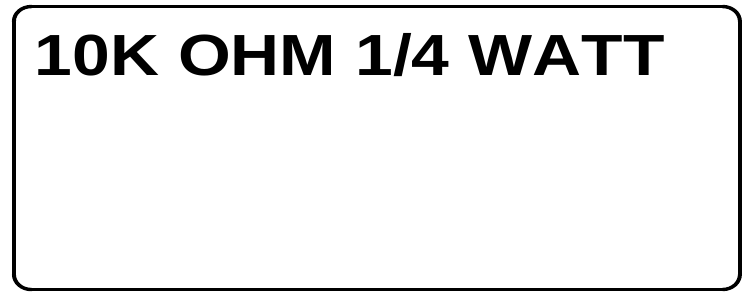
\includegraphics[scale=0.3]{./Figures/label_ej.png}
	\caption{Etiqueta resultante del comando de la columna Ejemplo de la tabla \ref{tab:printercmdSystem}.}
	\label{fig:label_ej}
\end{figure}

Se pueden enviar varias líneas a imprimir en un solo comando, en este caso para indicar el fin del texto se debe enviar E\textless{}CR\textgreater.

\subsection{Módulo adaptador RS-232}
\label{subsec:Mod232}
Para comunicar la impresora con la UART del microcontrolador se utilizó el módulo de la figura \ref{fig:rs232}. 

\begin{figure}[hb]
	\centering
	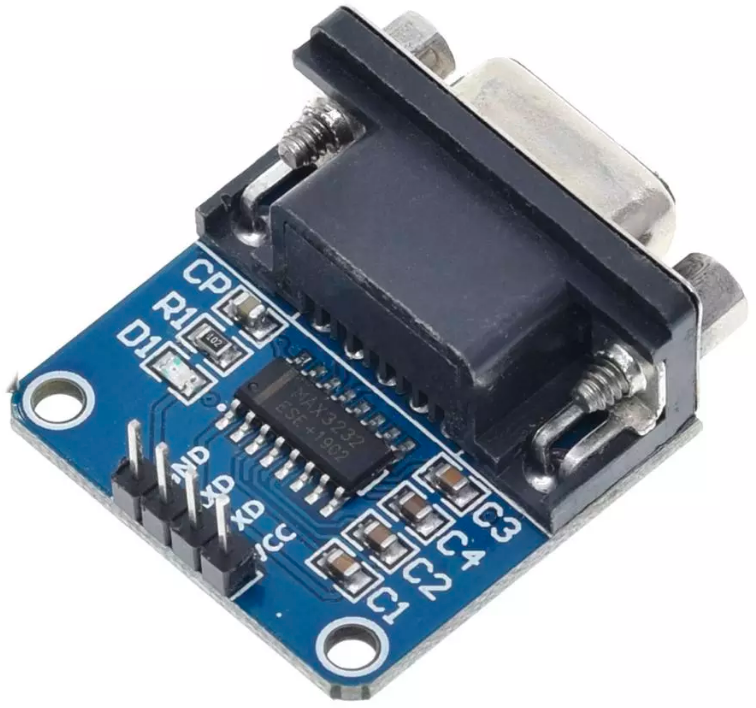
\includegraphics[scale=0.3]{./Figures/rs3232.png}
	\caption{Módulo adaptador RS-232 a TTL.}
	\label{fig:rs232}
\end{figure}

Este módulo está basado en el integrado MAX3232 \citep{MAX3232} y adapta las señales del capa física RS-232 a valores acordes para trabajar con el microcontrolador.

\section{Display alfanumérico}

Para este trabajo se utilizó un \textit{display} alfanumérico de 20 columnas por 4 líneas con controlador HD44780 de Hitachi \citep{HD44780}, ver figura \ref{fig:display}.

\begin{figure}[htpb]
	\centering
	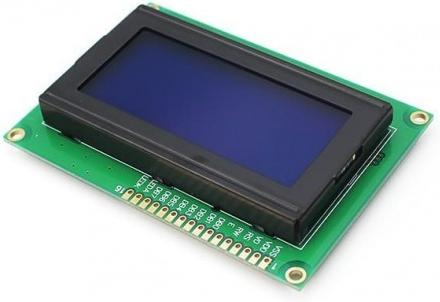
\includegraphics[scale=0.7]{./Figures/display.jpg}
	\caption{\textit{Display} alfanumérico de 20x4.}
	\label{fig:display}
\end{figure}

El display cuenta con una interfaz paralela de 8-bits (DB0-7) la cual puede ser utilizada en formato 4-bits haciendo 2 escrituras o lecturas. Cuenta también con tres líneas de control denominadas RS, R/W y EN. En la tabla \ref{tab:display} se muestran las señales necesarias para el manejo del \textit{display}.

\begin{table}[ht]
\centering
\caption[Señales de control y datos \textit{display}]{Señales de control y datos \textit{display}.}
\begin{tabular}{c c c}
\hline
\toprule
\textbf{Señal} & \begin{tabular}[c]{@{}c@{}}\textbf{Tamaño}\\ \textbf{bits}\end{tabular} & \textbf{Descripción} \\ 
\midrule
RS    & 1 & \begin{tabular}[c]{@{}c@{}}Indica como interpretar los datos en el \textit{bus} de datos DB.\\ 0: Instrucción\\ 1: Datos\end{tabular} \\
R/W   & 1 & \begin{tabular}[c]{@{}c@{}}0: Operación de lectura\\ 1: Operación de escritura\end{tabular} \\
EN    & 1 & \begin{tabular}[c]{@{}c@{}}\textit{Enable}: utilizado para indicar que hay \\ datos validos en el \textit{bus} de datos\end{tabular} \\
DB    & 8 & \textit{Bus} de datos \\
\bottomrule
\hline
\end{tabular}%
\label{tab:display}
\end{table}

Para utilizar el display se cuenta con 2 tipos de operaciones las cuales se diferencian por el bit de control RS:
\begin{itemize}
\item RS=0: Escribir/leer una instrucción.
\item RS=1: Escribir/leer un carácter ASCII.
\end{itemize}

\pagebreak

En la tabla \ref{tab:displayCmd} se muestran las instrucciones más utilizadas.

\begin{table}[htpb]
\centering
\caption[Instrucciones controlador HD44780]{Instrucciones más utilizadas para el controlador HD44780.}
\begin{tabular}{c c l}
\hline
\toprule
\textbf{Nombre} & \begin{tabular}[l]{@{}c@{}}\textbf{Valor}\\ \textbf{hexa}\end{tabular} & \textbf{Acción} \\ 
\midrule
Borrado         & 0x01 &  Borra la pantalla completa\\
Modo de entrada & 0x04 & \begin{tabular}[l]{@{}l@{}}Fijar dirección del cursor: izquierda o derecha\end{tabular} \\
\begin{tabular}[c]{@{}c@{}}Control de \\encendido y apagado\end{tabular} & 0x08 & \begin{tabular}[l]{@{}l@{}}- Encender o apagar la pantalla\\- Encender o apagar el cursor \end{tabular} \\
Fijar \textit{Set}    & 0x10 & \begin{tabular}[l]{@{}l@{}}- Fijar tamaño del \textit{bus} de datos \\- Fijar número de líneas \\- Fijar fuente de los caracteres \end{tabular} \\
\bottomrule
\hline
\end{tabular}%
\label{tab:displayCmd}
\end{table}

\section{Módulos misceláneos}

En esta sección se describe el módulo utilizado como elemento de maniobra para alimentar los bobinados del transformador y la fuente de alimentación utilizada en el trabajo.

\subsubsection{Módulo de relés}
\label{subsubsec:ModRel}

Para poder conmutar las tensiones aplicadas a los bobinados del transformador bajo ensayo se utilizó el módulo de la figura \ref{fig:reles} . Este módulo está compuesto por 8 relés los cuales pueden ser manejados en forma aislada por el microcontrolador a través de optoacopladores. Este módulo permitió actuar sobre las altas tensiones del transformador bajo ensayo de una manera segura.

\begin{figure}[htpb]
	\centering
	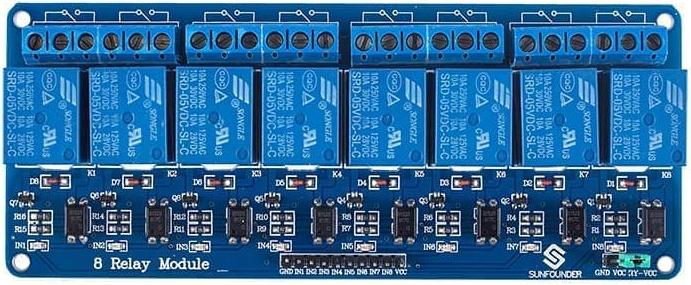
\includegraphics[scale=0.7]{./Figures/reles.jpeg}
	\caption{Módulo de relés.}
	\label{fig:reles}
\end{figure}

\pagebreak

\subsubsection{Módulo de alimentación}
\label{subsubsec:ModAlim}

El dispositivo diseñado debe ser alimentado desde la red eléctrica de Argentina (220 V$_{RMS}$ - 50 hz), para tal fin se utilizó la fuente conmutada mostrada en la figura \ref{fig:fte}.

\begin{figure}[htpb]
	\centering
	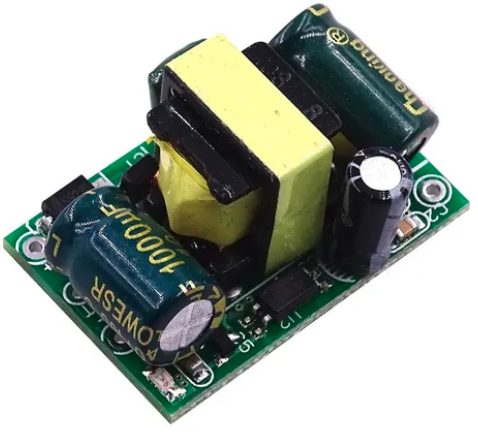
\includegraphics[scale=0.6]{./Figures/fte.png}
	\caption{Módulo de alimentación.}
	\label{fig:fte}
\end{figure}

Especificaciones técnicas tomadas de la pagina web del vendedor ya que no se pudieron encontrar los datos del fabricante del módulo:
\begin{itemize}
\item Tensión de entrada: 85 a 265 V$_{RMS}$ 50 hz.
\item Corriente de entrada: 0,0273 A (110 V$_{RMS}$) y 0,014 A (220 V$_{RMS}$).
\item Tensión de salida: 5 V +/- 0,2 V.
\item Corriente de salida: 700 mA (800 mA$_{PICO}$).
\item Ripple: 60 mV.
\item Potencia: 3,5 W.
\item Eficiencia: 80\%.
\item Protección contra corto circuito.
\item Temperatura de operación: -20 a 60 $^{\circ}$C.
\end{itemize}


% \footnote{\url{https://articulo.mercadolibre.com.ar/MLA-700576819-fuente-aislada-switching-220v-5v-700ma-35w-20off-nut-_JM\#reco_item_pos=2&reco_backend=machinalis-v2p-pdp-boost-v2&reco_backend_type=low_level&reco_client=vip-v2p&reco_id=90222827-7627-46cb-9f2b-78620eec7ea2}}
 
\chapter{Diseño e implementación} % Main chapter title

\label{Chapter3} % Change X to a consecutive number; for referencing this chapter elsewhere, use \ref{ChapterX}

\definecolor{mygreen}{rgb}{0,0.6,0}
\definecolor{mygray}{rgb}{0.5,0.5,0.5}
\definecolor{mymauve}{rgb}{0.58,0,0.82}

%%%%%%%%%%%%%%%%%%%%%%%%%%%%%%%%%%%%%%%%%%%%%%%%%%%%%%%%%%%%%%%%%%%%%%%%%%%%%
% parámetros para configurar el formato del código en los entornos lstlisting
%%%%%%%%%%%%%%%%%%%%%%%%%%%%%%%%%%%%%%%%%%%%%%%%%%%%%%%%%%%%%%%%%%%%%%%%%%%%%
\lstset{ %
  backgroundcolor=\color{white},   % choose the background color; you must add \usepackage{color} or \usepackage{xcolor}
  basicstyle=\footnotesize,        % the size of the fonts that are used for the code
  breakatwhitespace=false,         % sets if automatic breaks should only happen at whitespace
  breaklines=true,                 % sets automatic line breaking
  captionpos=b,                    % sets the caption-position to bottom
  commentstyle=\color{mygreen},    % comment style
  deletekeywords={...},            % if you want to delete keywords from the given language
  %escapeinside={\%*}{*)},          % if you want to add LaTeX within your code
  %extendedchars=true,              % lets you use non-ASCII characters; for 8-bits encodings only, does not work with UTF-8
  %frame=single,	                % adds a frame around the code
  keepspaces=true,                 % keeps spaces in text, useful for keeping indentation of code (possibly needs columns=flexible)
  keywordstyle=\color{blue},       % keyword style
  language=[ANSI]C,                % the language of the code
  %otherkeywords={*,...},           % if you want to add more keywords to the set
  numbers=left,                    % where to put the line-numbers; possible values are (none, left, right)
  numbersep=5pt,                   % how far the line-numbers are from the code
  numberstyle=\tiny\color{mygray}, % the style that is used for the line-numbers
  rulecolor=\color{black},         % if not set, the frame-color may be changed on line-breaks within not-black text (e.g. comments (green here))
  showspaces=false,                % show spaces everywhere adding particular underscores; it overrides 'showstringspaces'
  showstringspaces=false,          % underline spaces within strings only
  showtabs=false,                  % show tabs within strings adding particular underscores
  stepnumber=1,                    % the step between two line-numbers. If it's 1, each line will be numbered
  stringstyle=\color{mymauve},     % string literal style
  tabsize=2,	                   % sets default tabsize to 2 spaces
  title=\lstname,                  % show the filename of files included with \lstinputlisting; also try caption instead of title
  morecomment=[s]{/*}{*/}
}

\lstset{literate=
  {á}{{\'a}}1 {é}{{\'e}}1 {í}{{\'i}}1 {ó}{{\'o}}1 {ú}{{\'u}}1
  {Á}{{\'A}}1 {É}{{\'E}}1 {Í}{{\'I}}1 {Ó}{{\'O}}1 {Ú}{{\'U}}1
}

En el presente capítulo se describen el hardware y firmware implementados en el trabajo. Se detalla la integración de los módulos de hardware presentados en el capítulo anterior con el kit ESP32-DevKitC. Luego, se presenta el desarrollo del firmware y se fundamentan las decisiones tomadas en el diseño.

%----------------------------------------------------------------------------------------
%	SECTION 1
%----------------------------------------------------------------------------------------
\section{Descripción de hardware}
En esta sección se detalla como se conectaron los diferentes módulos de hardware presentados en el capítulo \ref{Chapter2} con el kit ESP32-DevKitC. En la figura \ref{fig:conexionado} se muestra un diagrama de conexionado entre el kit ESP32-DevKitC y los diferentes módulos.

\begin{figure}[htpb]
	\centering
	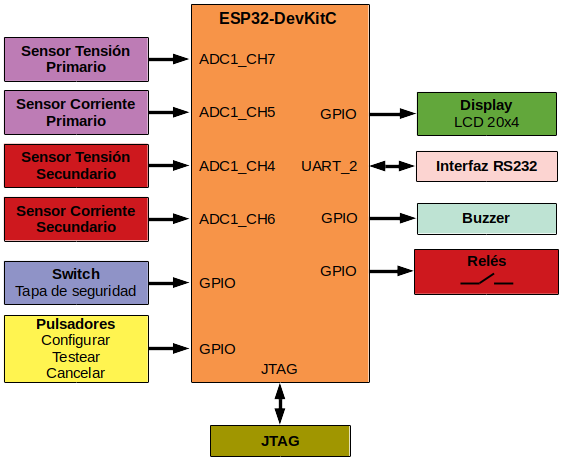
\includegraphics[scale=0.7]{./Figures/diagrama_det.png}
	\caption{Conexionado kit ESP32-DevKitC y módulos de hardware.}
	\label{fig:conexionado}
\end{figure}

Para el conexionado de los elementos del sistema se utilizó una placa universal de 90 mm x 150 mm. Esta permitió un rápido conexionado de los módulos con el kit y la posibilidad de trabajar con hardware y software sin la necesidad de contar con todo el hardware diseñado y construido. En la placa universal se montaron los siguientes componentes:

\begin{itemize}
\item Kit ESP32-DevKitC.
\item Dos fuentes de alimentación de 220 V$_{RMS}$ a 5 V (sección \ref{subsubsec:ModAlim}).
\item El \textit{buzzer}. 
\item Componentes varios necesarios para el apropiado funcionamiento de los módulos analógicos con el kit de desarrollo.
\item Diferentes conectores tipo \textit{header} para el conexionado de los módulos de hardware presentados en el capítulo \ref{Chapter2}.
\end{itemize}

En la tabla \ref{tab:diagramaPines} se muestra el uso de los pines del kit ESP32-DevKitC. En general, todos los módulos fueron conectados directamente al kit con la excepción de los módulos sensores de tensión y corriente cuyo conexionado requirió divisores resistivos para adaptar los valores de salida de los módulos al rango de excursión del ADC. A su vez que si incluyó en la placa universal una referencia de tensión basada en el integrado TL431 \citep{TL431}, esto se explica con más detalle en la sección \ref{subsec:mejorasAnalo}.

\begin{table}[htpb]
\centering
\caption[Uso de pines del kit ESP32-DevKitC]{Uso de los pines del kit ESP32-DevKitC.}
\begin{tabular}{c c c}
\hline
\toprule
\textbf{Pines kit} & \textbf{Módulo}                        & \textbf{Símbolo}      \\ \hline
\multicolumn{3}{c}{Medición de corrientes y tensiones del transformador}   \\ \hline
IO35/ADC1\_CH7     & Sensor de tensión primario             & PV           \\
IO33/ADC1\_CH5     & Sensor de corriente primario           & PC           \\
IO32/ADC1\_CH4     & Sensor de tensión secundario           & SV           \\
IO34/ADC1\_CH6     & Sensor de corriente secundario         & SC           \\
IO25               & Alimentación bobinado primario         & CPV          \\
IO26               & Alimentación bobinado secundario       & CSV          \\ \hline
\multicolumn{3}{c}{\textit{Display}}                                       \\ \hline
IO18               & \textit{Enable}                        & EN           \\
IO5                & RS                                     & RS           \\
IO19               & \textit{Bus} de datos bit 4            & D4           \\
IO21-23            & \textit{Bus} de datos bits 5 a 7       & D5-7         \\ \hline
\multicolumn{3}{c}{Interfaz RS232}                                         \\ \hline
IO16/RXD2          & Recepción                              & RX           \\
IO17/TXD2          & Transmisión                            & TX           \\ \hline
\multicolumn{3}{c}{Pulsadores}                                             \\ \hline
IO39               & Testear                                & PTEST        \\
IO36               & Configurar                             & PCONF        \\
IO27               & Cancelar                               & PCAN         \\ \hline
\multicolumn{3}{c}{Otros}                                                  \\ \hline
IO4                & \textit{Buzzer}                        & BUZZ         \\
IO2                & \textit{Switch} de seguridad           & SWITCH       \\
IO12-15            & JTAG                                   & -            \\ 
\bottomrule
\hline
\end{tabular}%
\label{tab:diagramaPines}
\end{table}

\subsection{Mejoras a las entradas analógicas}
\label{subsec:mejorasAnalo}
En las secciones \ref{sec:secZMPT101B} y \ref{sec:secZMCT103C} se introdujeron los módulos de hardware sensores de tensión y corriente. Estos módulos son muy prácticos debido a que proporcionan valores de tensiones acordes para trabajar con el ADC del kit ESP32-DevKitC y, a su vez, proporcionan aislamiento eléctrico de las altas tensiones de los bobinados. Sin embargo, al mirar con más detalle los módulos, se pueden identificar las siguientes desventajas:
\begin{enumerate}
\item El amplificador LM358 tiene saturaciones fuertemente asimétricas, V$_{SAT+}$ = Vcc-1,5 V @ Vcc = 5 V y V$_{SAT-} \simeq $  0 V @ Vcc = 5 V. Teniendo en cuenta que el \textit{offset} de salida de los módulos está a la mitad de la alimentación, la saturación positiva limita la excursión de los módulos y por lo tanto, el rango aprovechable del ADC, figura \ref{fig:sensSat}. 
\item En el caso del sensor de corriente, este no posee \textit{offset} en la salida, esto genera tensiones negativas incompatibles con el ADC del kit.
\item La tensión de alimentación se utiliza como tensión de referencia para generar los 2,5 V de \textit{offset} a la salida del módulo. Si esta tensión no es estable, toda la medición se verá comprometida.
\end{enumerate}

\begin{figure}[htpb]
	\centering
	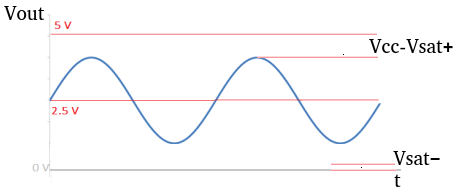
\includegraphics[scale=1]{./Figures/ZMPT101B_waves_sat.png}
	\caption{Saturación módulos sensores.}
	\label{fig:sensSat}
\end{figure}

Luego de estudiar los circuitos, se decidió tomar las siguientes acciones para solucionar los problemas encontrados:
\begin{enumerate}
\item Se modificó el divisor resistivo que fijaba la tensión de \textit{offset} en la mitad de la alimentación a un valor más acorde, figura \ref{fig:sensSatMej}.
\item Se eliminó el capacitor de desacople serie que estaba en la salida del sensor de corriente. Esto permitió que la salida de este módulo excursione solo entre valores positivos.
\item Se decidió alimentar los módulos con una referencia de tensión (TL431 \citep{TL431}) en vez de utilizar la tensión de alimentación de la fuente generada en la placa universal.
\end{enumerate}

\begin{figure}[htpb]
	\centering
	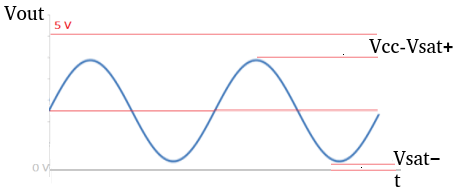
\includegraphics[scale=1]{./Figures/ZMPT101B_waves_sat_mod.png}
	\caption{Saturación mejorada.}
	\label{fig:sensSatMej}
\end{figure}


\subsection{Integración de hardware}

En la figura \ref{fig:gab1} se muestra el trabajo realizado. Como se puede notar, este consta de dos gabinetes los cuales están conectados por cables que se  observan en la parte derecha de la figura. 

\begin{figure}[htpb]
	\centering
	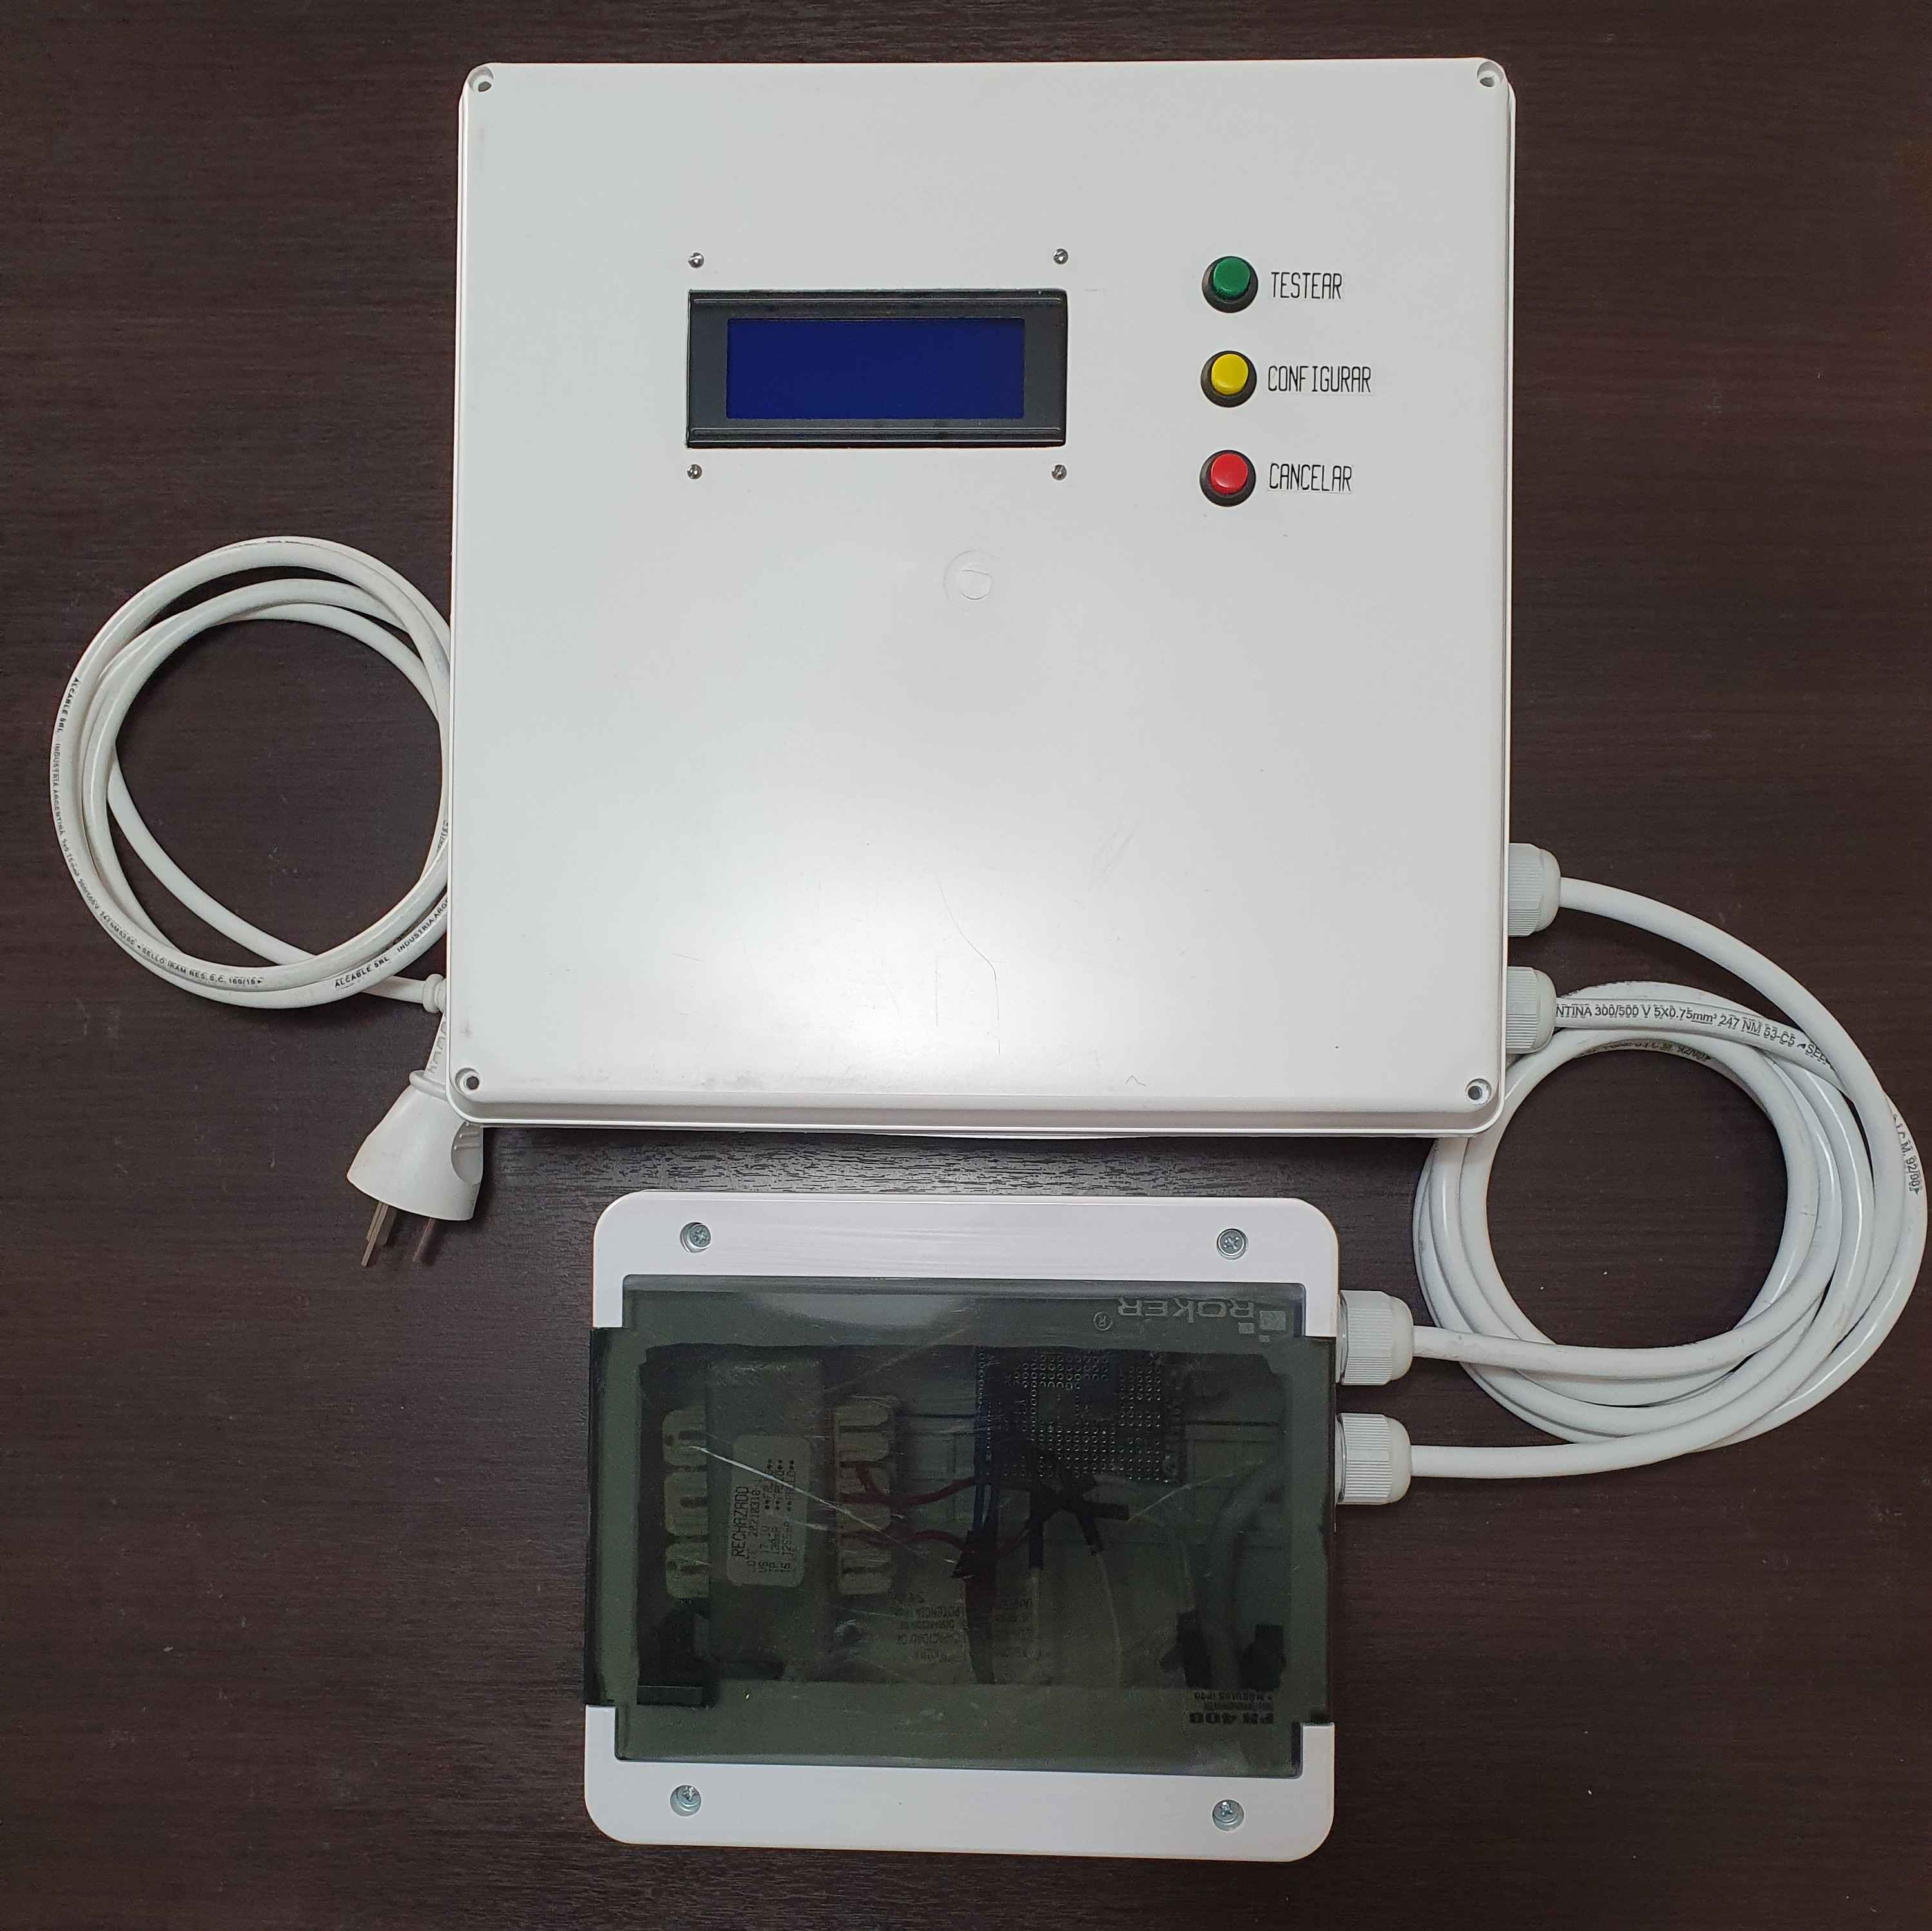
\includegraphics[scale=0.16]{./Figures/gab1.jpg}
	\caption{Trabajo final terminado.}
	\label{fig:gab1}
\end{figure}

En el gabinete de la parte superior de la figura, denominado gabinete principal, se encuentran los diferentes módulos presentados en el capítulo \ref{Chapter2} los cuales son conectados al kit ESP32-DevKitC a través de la placa universal. Por otro lado, el gabinete de la parte inferior, denominado gabinete auxiliar, está destinado a albergar el transformador que se desea ensayar. En la figura, además, se pueden observar el \textit{display} alfanumérico y los tres pulsadores los cuales fueron rotulados acorde a su función. 

Como se dijo, en el gabinete auxiliar debe ser colocado el transformador a ensayar, para esto, este cuenta con una tapa gris denominada tapa de seguridad. En la figura \ref{fig:gab2} se muestran los mismos gabinetes pero se encuentra la tapa de seguridad abierta y se aprecia un transformador de prueba colocado en dicho gabinete. 

\begin{figure}[h]
	\centering
	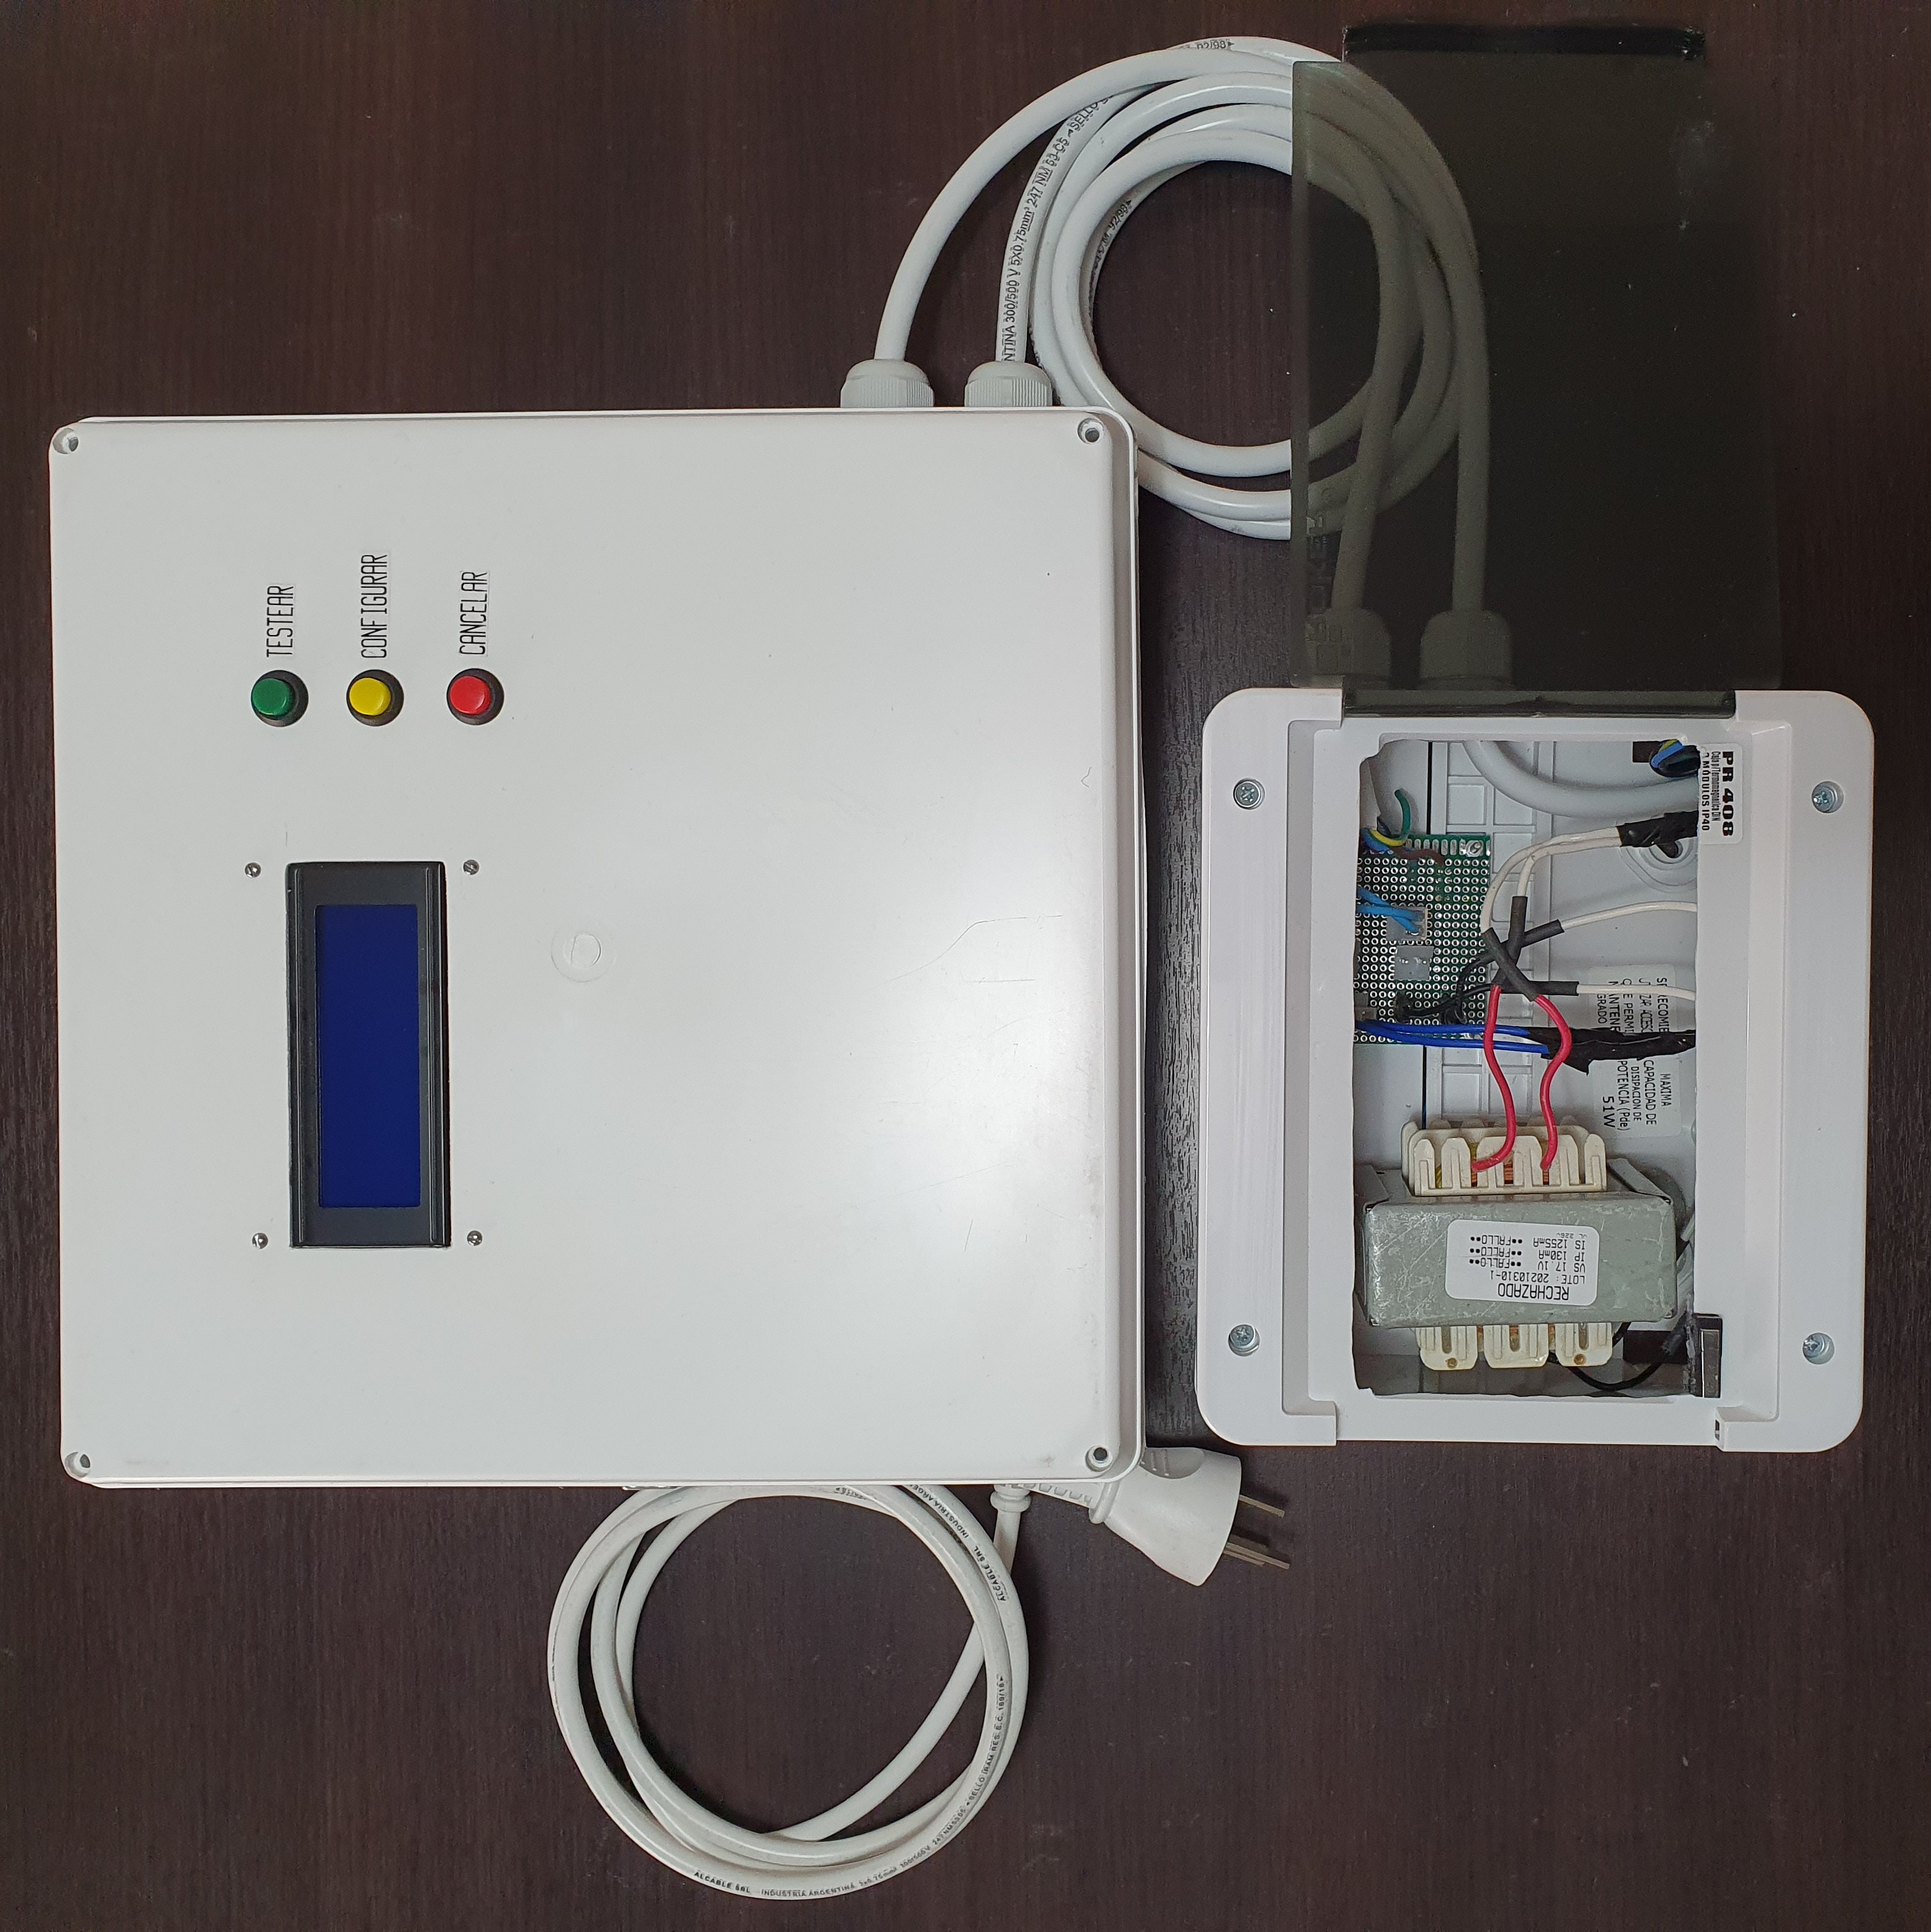
\includegraphics[scale=0.16]{./Figures/gab2.jpg}
	\caption{Trabajo terminado con la tapa de seguridad abierta.}
	\label{fig:gab2}
\end{figure}

\pagebreak

En la figura \ref{fig:gab3} se muestra el gabinete principal sin la tapa. Se pueden distinguir los siguientes componentes:

\begin{itemize}
\item Placa universal con el kit ESP32-DevKitC y componentes asociados.
\item Dos módulos sensores de tensión, sección \ref{sec:secZMPT101B}.
\item Dos módulos sensores de corriente, sección \ref{sec:secZMCT103C}.
\item El módulo de relés, sección \ref{subsubsec:ModRel}.
\item El módulo adaptador RS232, sección \ref {subsec:Mod232}.
\item Un transformador que se utiliza como transformador auxiliar para generar la tensión alterna necesaria para alimentar el transformador bajo prueba.
\end{itemize}

Es importante destacar que el armado de los gabinetes fue realizado desde cero con las herramientas disponibles en el hogar. Este demandó mucho tiempo, esfuerzo y dedicación. Aún cuando no es el objetivo del posgrado el armado de gabinetes, creo que es importante resaltar este punto ya que el trabajo terminado, a pesar de ser un prototipo, está en condiciones de ser utilizado como instrumento de medición en un ambiente industrial.

\begin{figure}[h]
	\centering
	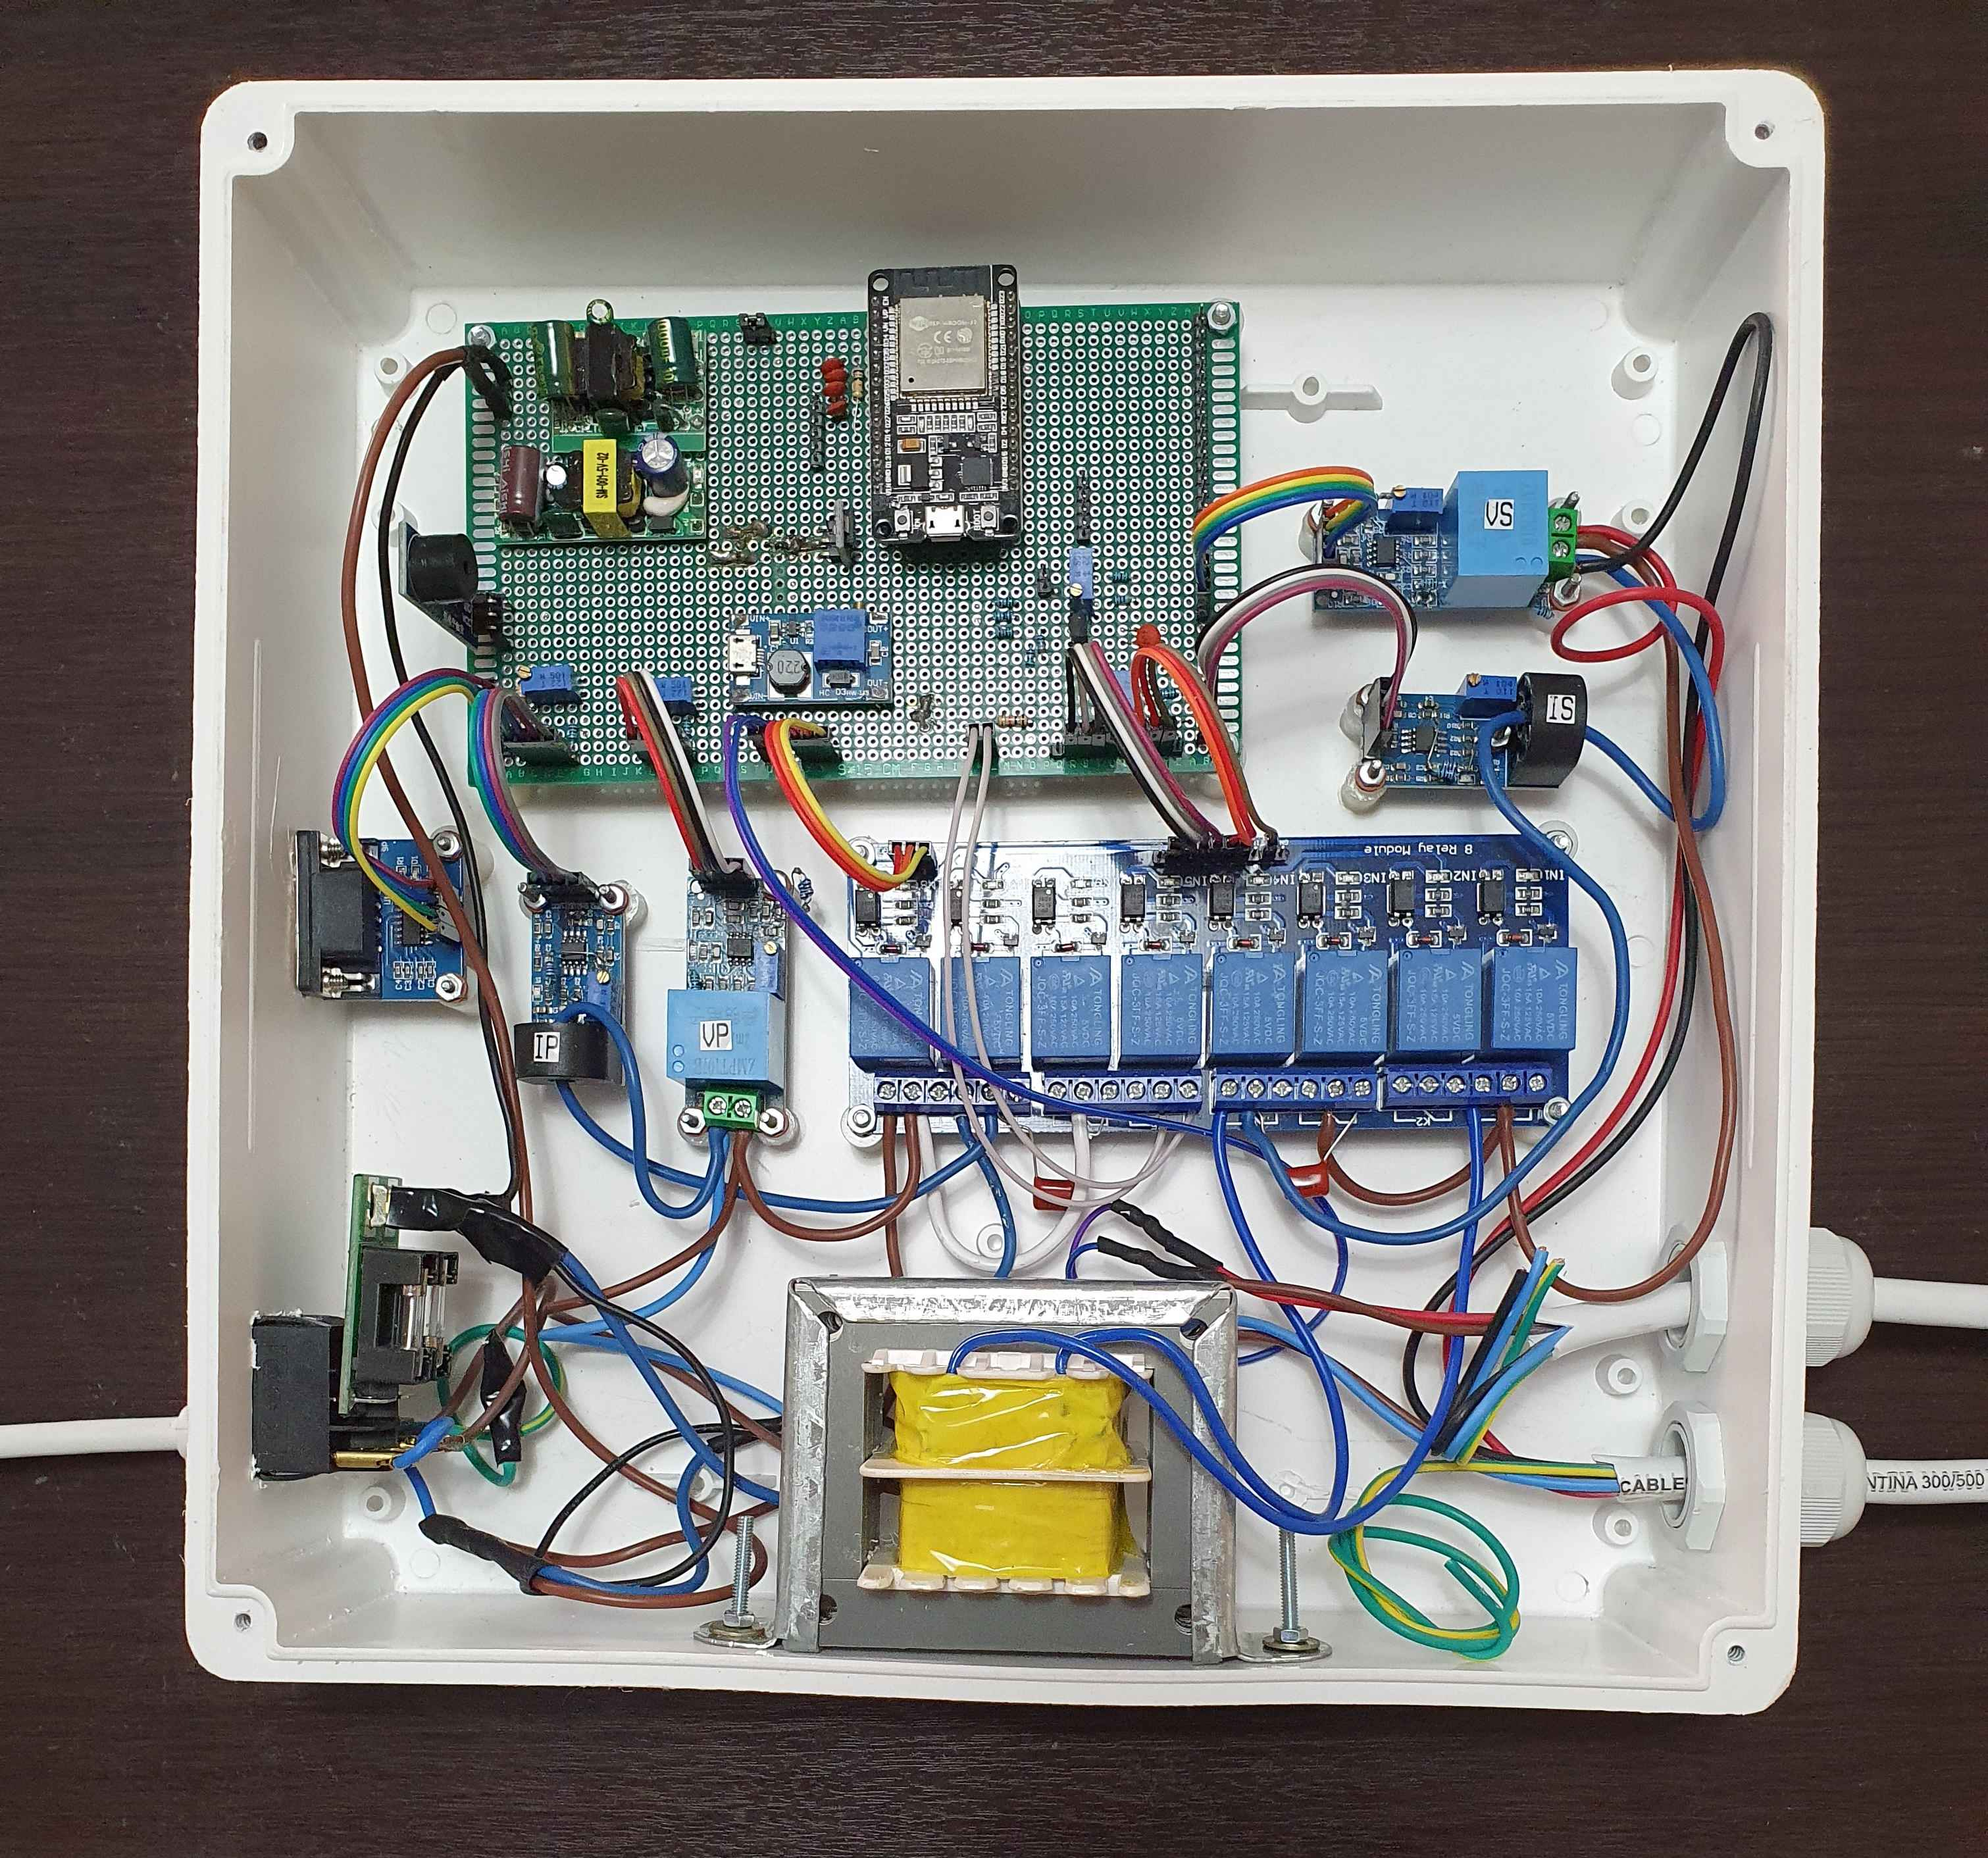
\includegraphics[scale=0.15]{./Figures/gab3.jpg}
	\caption{Contenido gabinete principal.}
	\label{fig:gab3}
\end{figure}

\pagebreak

En la figura \ref{fig:gab4} se muestra el gabinete auxiliar donde se pueden observar los diferentes conectores para el conexionado del transformador a ensayar.

\begin{figure}[hb]
	\centering
	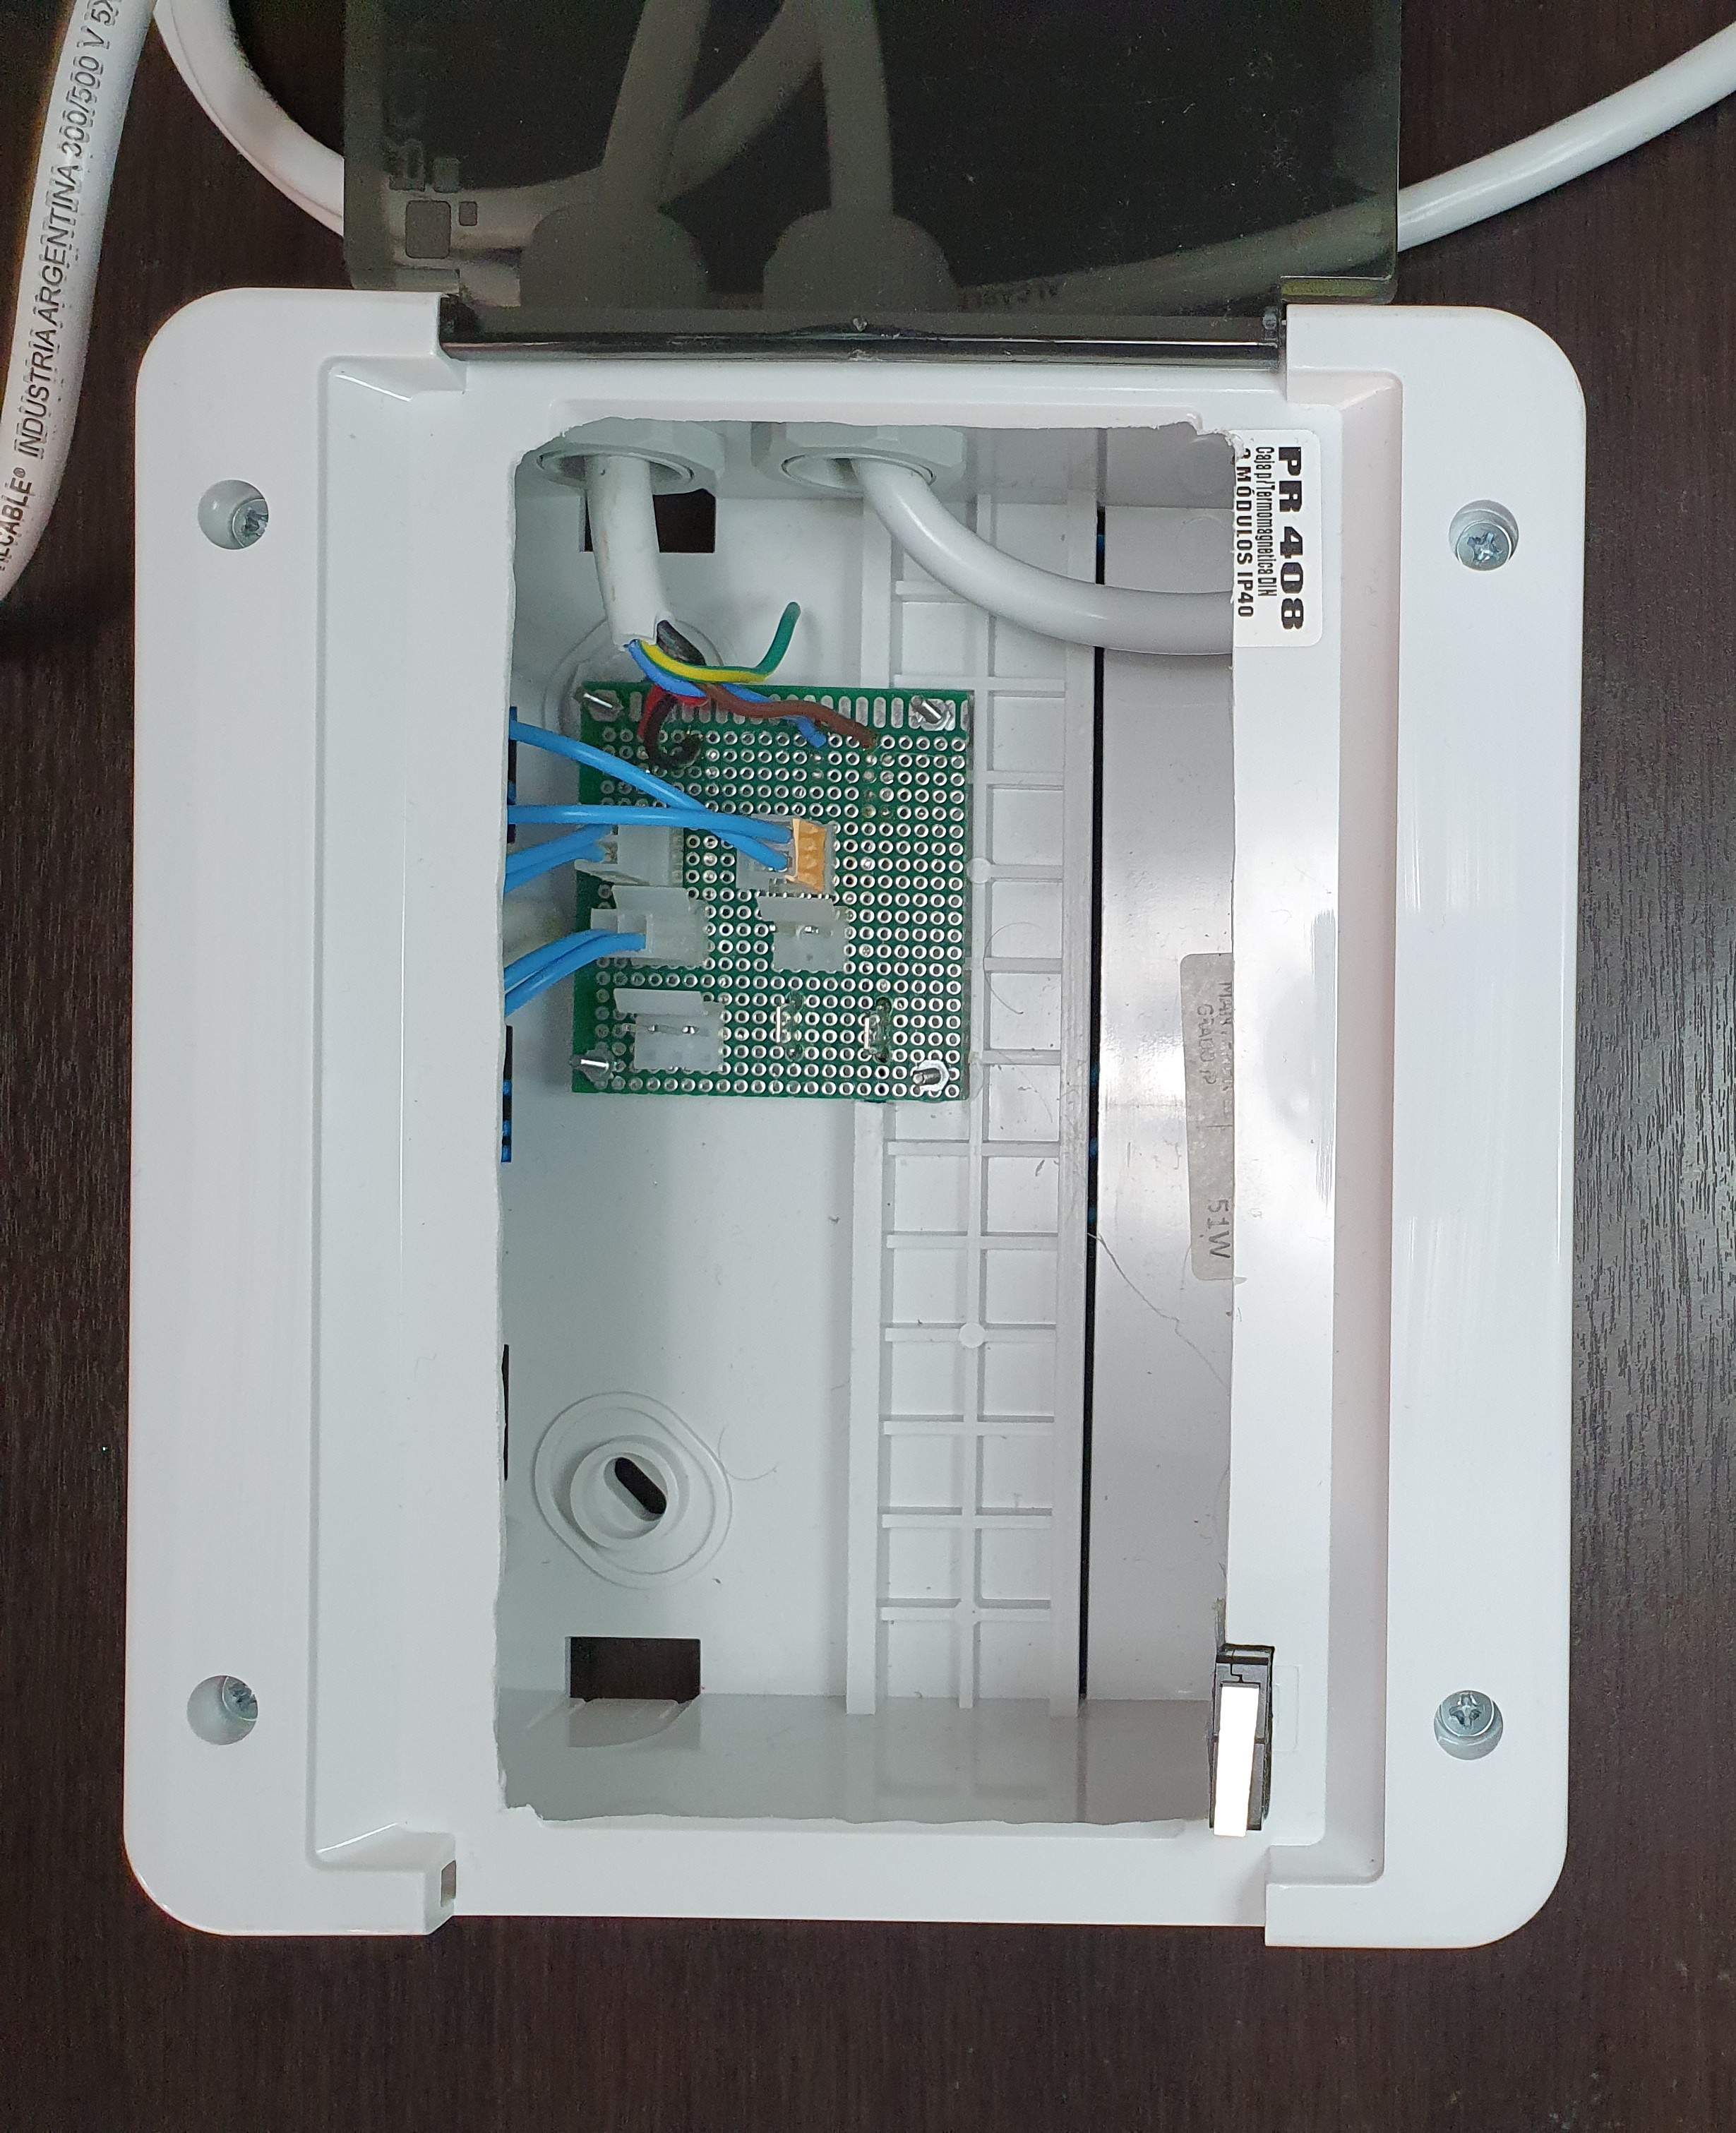
\includegraphics[scale=0.08]{./Figures/gab4.jpg}
	\caption{Gabinete auxiliar sin el transformador a ensayar.}
	\label{fig:gab4}
\end{figure}


\section{Descripción de firmware}

En esta sección se describe la arquitectura de firmware adoptada, así como los módulos principales que la componen, se brinda detalle de las diferentes implementaciones y se destacan sus aspectos más importantes.

\subsection{Arquitectura de firmware}
Luego de analizar posibles patrones de arquitectura de software a utilizar, se decidió utilizar el patrón observar y reaccionar visto en Ingeniería de Software \citep{INGSOFT}, figura \ref{fig:patron}. Este patrón se utiliza cuando un conjunto de sensores se monitorean y muestran de manera rutinaria.

\begin{figure}[htpb]
	\centering
	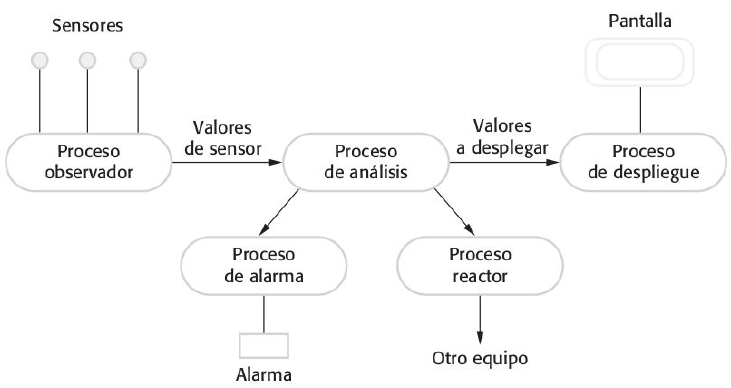
\includegraphics[scale=0.55]{./Figures/patron.png}
	\caption{Patrón observar y reaccionar.}
	\label{fig:patron}
\end{figure}

El dispositivo diseñado responde muy bien a esta arquitectura ya que se deben monitorear los sensores (pulsadores, monitores de tensiones y corrientes), accionar actuadores y enviar los resultados a procesos de salida (\textit{display}, servidor web e impresora). En ningún momento se tienen lazos de realimentación o estructuras que rompan la secuencialidad del sistema. En la figura \ref{fig:patronAplicado} se muestra el patrón aplicado al trabajo.

\begin{figure}[htpb]
	\centering
	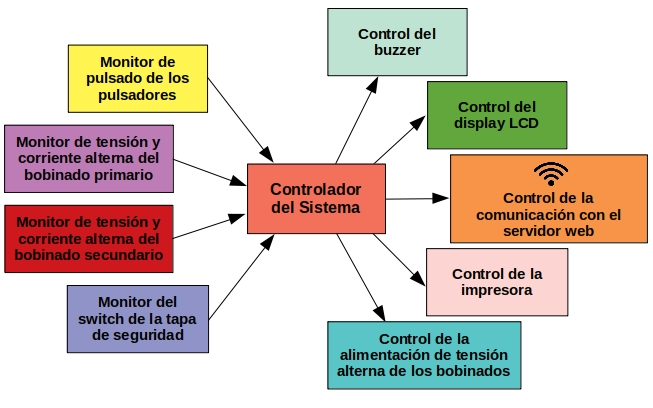
\includegraphics[scale=0.55]{./Figures/arquitecturaSoft.jpg}
	\caption{Patrón observar y reaccionar aplicado al trabajo.}
	\label{fig:patronAplicado}
\end{figure}



\subsection{Estructura general del firmware}

El firmware fue desarrollado por medio de la utilización de buenas prácticas de programación como por ejemplo el control de versiones, la modularización y la documentación en el código fuente. Para llevar adelante el control de versiones se creó un repositorio en GitHub \citep{TP_CESE} desde el inicio del trabajo. En cuanto a la modularización, se creó una estructura de módulos/archivos como la siguiente:

\dirtree{%
.1 TP\_CESE.
.2 inc.
.3 app\_adc.h.
.3 app\_Comm.h.
.3 ...
.2 sch.
.2 src.
.3 app\_adc.c.
.3 app\_Comm.c.
.3 ...
.3 main.c.
.3 ...
.2 .gitignore.
.2 CMakeLists.txt.
.2 sdkconfig.
.2 Doxyfile.
.2 README.md.
}

Donde: 
\begin{itemize}
\item inc: directorio para ubicar todos los archivos de cabeceras.
\item sch: directorio con el esquemático de la placa universal en KiCad \citep{KICAD}.
\item src: directorio para ubicar todos los archivos fuentes.
\item CMakeLists.txt: es el archivo principal que usa CMake para construir el proyecto.
\item sdkconfig: este archivo contiene la configuración de todos los componentes del proyecto (incluido ESP-IDF).
\item Doxyfile: archivo de configuración para generar la documentación a través de Doxygen.
\end{itemize}

A continuación se detallan los principales módulos de software desarrollados desde la perspectiva de su archivo de cabecera:

\begin{itemize}
\item adc.h: implementación del manejo de los ADCs para leer los tensiones y corrientes de los bobinados.
\item app\_Comm.h: se utiliza para ``parsear'' los paquete HTTP enviados y recibidos desde el servidor web.
\item app\_error.h: se utiliza para definir un criterio de error común frente a las diferentes fallas del sistema.
\item app\_fsm.h: máquina de estado del controlador principal.
\item app\_gpio.h: se utiliza para definir las diferentes funciones para el manejo de entradas-salidas de propósito general como por ejemplo los pulsadores, el comando de alimentación de bobinados, etc.
\item app\_lcd.h: define las rutinas necesarias para escribir mensajes en el \textit{display}.
\item app\_printer.h: implementación del protocolo DPL y manejo del puerto RS232.
\item app\_WiFi.h: implementación de las diferentes rutinas para el manejo del protocolo Wi-Fi.
\item http\_client.h: implementación de las diferentes rutinas para el manejo del protocolo HTTP.
\item main.h: punto de entrada al firmware, inicializa todos los módulos de hardware.
\item test\_status.h: define diferentes macros y tipos de datos utilizados para almacenar el estado de los ensayos.
\end{itemize}

Por otro lado, se utilizó Doxygen para documentar el código fuente \citep{DOXYGEN}.

\subsection{Controlador de sistema}

Este es el bloque más importante y su función principal es coordinar la interacción de los módulos restantes. Está basado en una máquina de estados finita (FSM por sus siglas en inglés) que, en función de las variables monitoreadas, actúa sobre las controladas, figura \ref{fig:patronAplicado}.

Las funciones del bloque se detallan a continuación:

\begin{itemize}
\item Procesar el estado de los pulsadores Testear y Cancelar para iniciar y/o detener la secuencia de caracterización.
\item Procesar el estado del pulsador Configurar para leer los umbrales de validación para el transformador en ensayo.
\item Procesar los valores leídos de las tensiones y corrientes de los bobinados primario y secundario.
\item Procesar el estado del \textit{switch} de la tapa de seguridad.
\item Generar el comando para alimentar los bobinados.
\item Generar la información para mostrar en el \textit{display} local.
\item Enviar el estado de la medición al \textit{buzzer} para generar las secuencias de sonidos adecuadas.
\item Enviar o solicitar datos al servidor web.
\end{itemize}

En la figura \ref{fig:MainFSM_red} se muestra un diagrama simplificado del controlador. Los estados fueron enumerados para ayudar en la explicación.

En las siguientes secciones se explica en detalle cada estado y su interacción con los diferentes módulos del sistema. Cabe aclarar que no se abordan detalle tales como los motivos por los cuales falló la comunicación con la impresora o la comunicación Wi-Fi ya que estos son detallados en los capítulos posteriores, solo se explica como los resultados de los diferentes bloques impactan sobre el funcionamiento del controlador principal.
\pagebreak
\begin{figure}[ht]
	\centering
	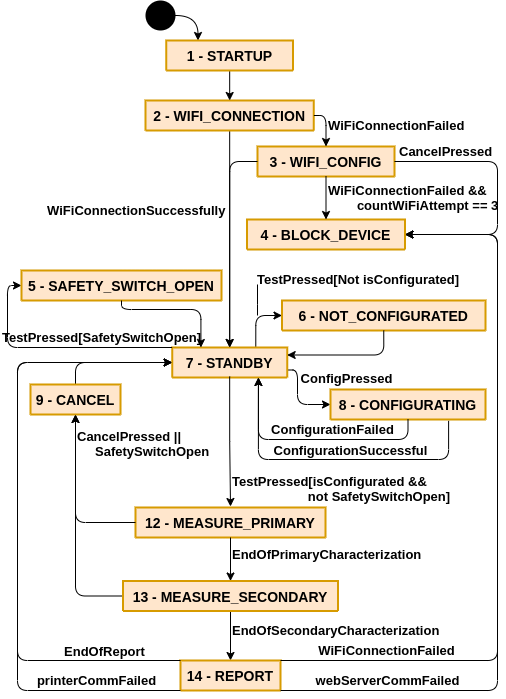
\includegraphics[scale=1]{./Figures/MainFSM_red.png}
	\caption{Diagrama simplificado del controlador del sistema.}
	\label{fig:MainFSM_red}
\end{figure}

Para una mejor explicación, se divide a la FSM en diferentes etapas donde cada una agrupa algunos estados:
\begin{itemize}
\item Etapa de inicialización: estados 1, 2 y 3.
\item Etapa de configuración: estados 6, 8, 10 y 11, estos últimos no se muestran en la figura \ref{fig:MainFSM_red} por claridad.
\item Etapa de caracterización: estados 5, 9, 12, 13 y 14.
\item Etapa de reporte: estado 14.
\end{itemize}

Los estados 7 (\textit{STANDBY}) y 4 (\textit{BLOCK\_DEVICE}) se consideran estados particulares y aparecen en todas o casi todas las etapas presentadas. Estos estados se consideran inicio y/o fin de las diferentes etapas.

\subsubsection{Etapa de inicialización}
\label{subsubsec:EtIni}
En la figura \ref{fig:MainFSM_1} se muestra la sub-máquina de estado correspondiente a la etapa de inicialización. 

\begin{figure}[htpb]
	\centering
	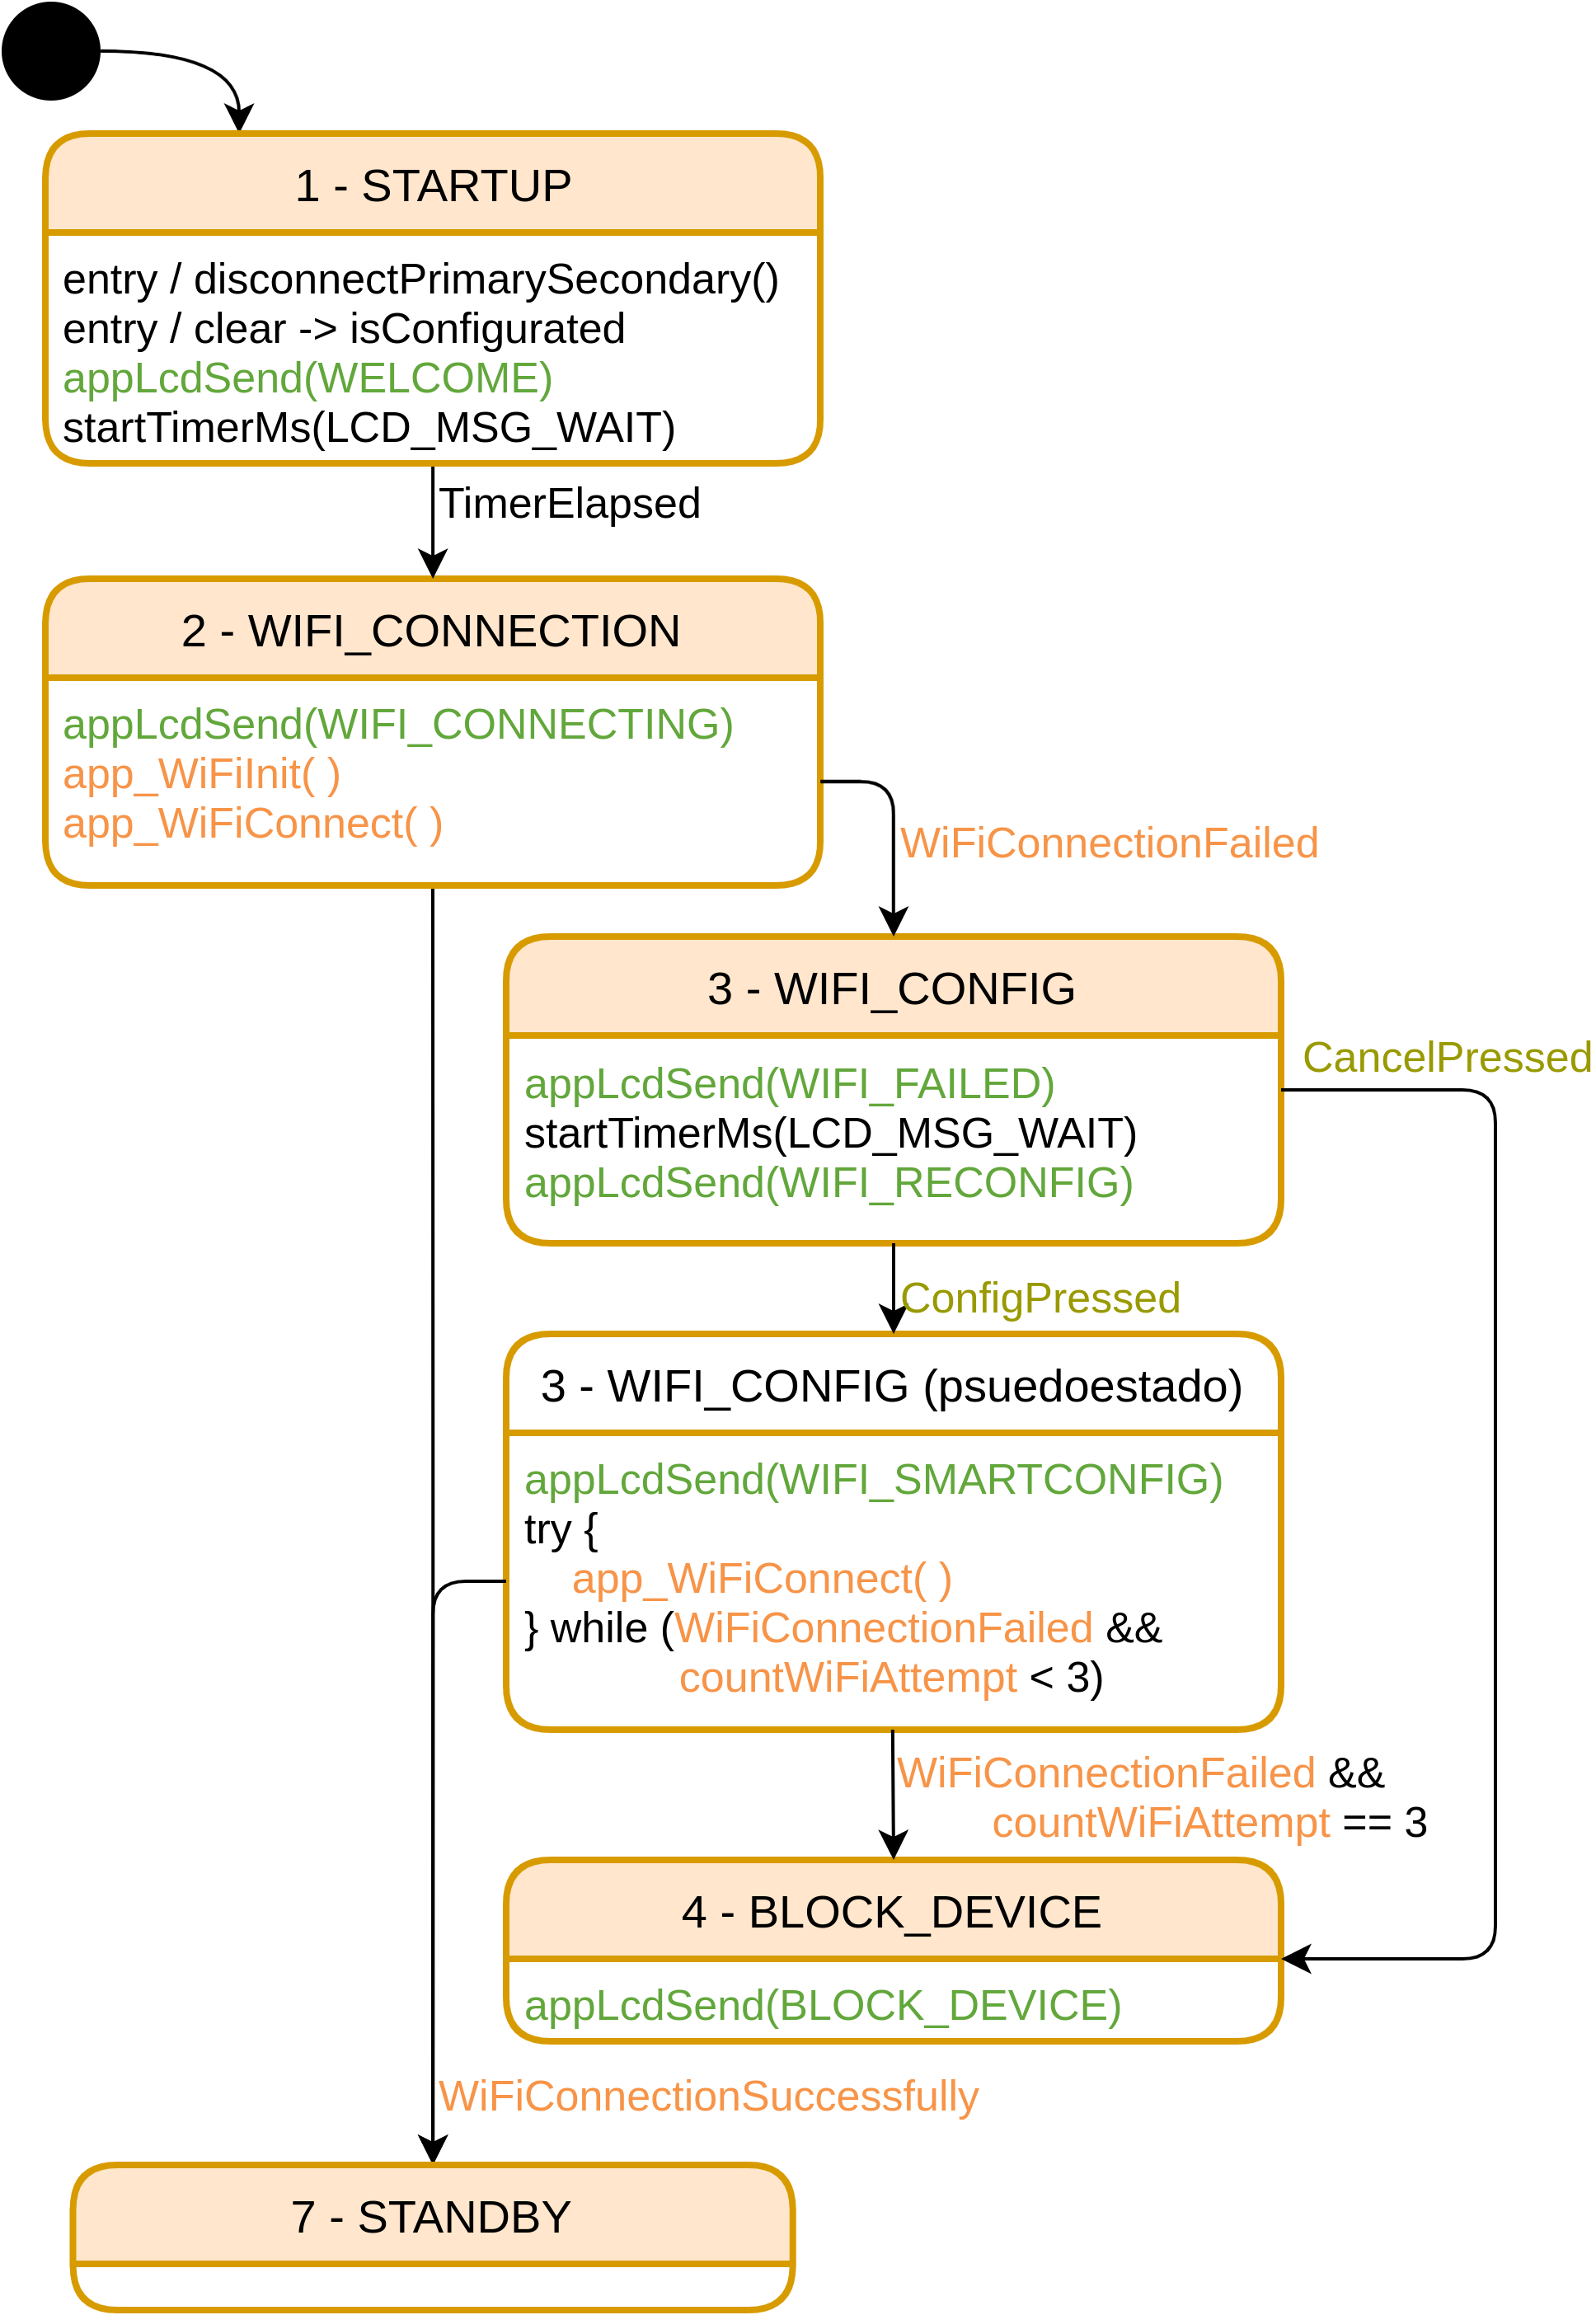
\includegraphics[scale=1]{./Figures/MainFSM_1.png}
	\caption{Etapa de inicialización.}
	\label{fig:MainFSM_1}
\end{figure}

Esta etapa se inicia cuando el equipo es energizado (salida de \textit{reset}) y termina en el estado 7 (\textit{STANDBY}) si el equipo fue exitoso al conectarse a Wi-Fi o en el estado estado 4 (\textit{BLOCK\_DEVICE}) si los intentos de conexión fallaron. 

Luego de la salida de \textit{reset} del sistema y de inicializar todos los módulos de hardware, se ingresa en el estado 1 (\textit{STARTUP}). Este estado tiene como función inicializar cuestiones de la máquina de estado principal como la alimentación de bobinados, mostrar un mensaje de bienvenida en el \textit{display} durante un tiempo fijo (\textit{LCD\_MSG\_WAIT}) y limpiar la variable \textit{isConfigurated}. Esta última se utiliza para indicar si el equipo fue configurado, al salir de \textit{reset} el equipo no se encuentra configurado.

Luego de transcurrido el tiempo \textit{LCD\_MSG\_WAIT}, se transiciona al estado 2 (\textit{WIFI\_CONNECTION}). En este estado, se leen los valores SSID y la contraseña desde la memoria no volátil del dispositivo y se intenta conectar a la red Wi-Fi configurada. En caso de fallar la conexión, se genera el evento \textit{WiFiConnectionFailed} y se transciona hacia el estado 3 (\textit{WIFI\_CONFIG}). 

En el estado \textit{WIFI\_CONFIG} se consulta si se desea reconfigurar las credenciales de Wi-Fi, para lo cual, el operador puede acceder al pulsar Configurar o negarse al pulsar Cancelar. En caso de reconfigurar, se utiliza la aplicación ESP-Touch \ref{sec:ESPTouch}, se realizan 3 intentos de reconexión y en caso de fallar nuevamente el equipo pasa al estado 4 (\textit{BLOCK\_DEVICE}) y finaliza la secuencia de inicio.

En caso de lograr la conexión Wi-Fi, sea en el estado 2 (\textit{WIFI\_CONNECTION}) o el psuedoestado 3 (\textit{WIFI\_CONFIG}), el sistema pasa al estado 7 (\textit{STANDBY}) y finaliza la secuencia de inicio.

\subsubsection{Etapa de configuración}
\label{subsubsec:EtConf}
En la figura \ref{fig:MainFSM_2} se muestra la sub-máquina de estado correspondiente a la etapa de configuración. 

Luego de la etapa de inicialización se ingresa en la etapa de configuración. Esta etapa se inicia y finaliza en el estado 7 (\textit{STANDBY}) y tiene dos funciones principales:

\begin{itemize}
\item Validar si el equipo fue configurado, por medio de \textit{isConfigurated}, para permitir pasar a la etapa de caracterización.
\item Pedir los datos de configuración al servidor web al pulsar Configurar y fijar el valor de \textit{isConfigurated} acorde al resultado de dicha acción.
\end{itemize}

En el estado 7 (\textit{STANDBY}) se muestra en el \textit{display} si el equipo fue o no configurado previamente en base al valor de \textit{isConfigurated}. Si el operario desea testear un transformador, para lo cual pulsa Testear, pero la variable \textit{isConfigurated} es cero, el equipo pasa al estado 6 (\textit{NOT\_CONFIGURATED}), muestra un mensaje de equipo no configurado y vuelve al estado \textit{STANDBY}.

Si el operario desea configurar el equipo debe pulsar Configurar, para la cual se pasa del estado \textit{STANDBY} al estado 8 (\textit{CONFIGURATING}). En este estado, se solicitan los valores de configuración al servidor web desarrollado por el cliente. De aquí, se pueden generar dos eventos posibles \textit{ConfigurationSuccessful} o \textit{ConfigurationFailed} que dependen de la obtención de los datos con o sin errores desde el servidor web. En ambos casos, se asigna el valor correcto a la variable \textit{isConfigurated} y se muestra en el \textit{display} el resultado.

\begin{figure}[ht]
	\centering
	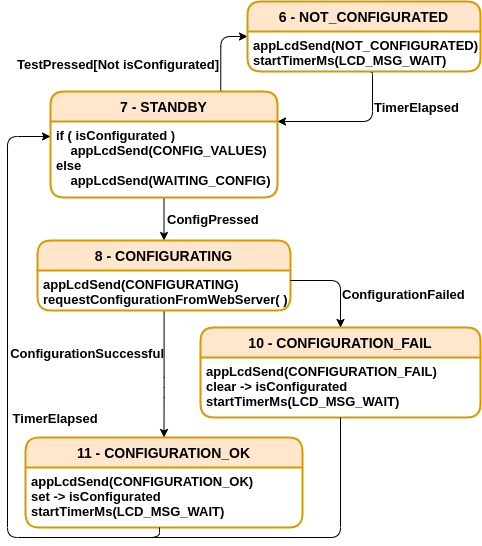
\includegraphics[scale=1]{./Figures/MainFSM_2.png}
	\caption{Etapa de configuración.}
	\label{fig:MainFSM_2}
\end{figure}

\subsubsection{Etapa de caracterización}
\label{subsubsec:EtTest}
En la figura \ref{fig:MainFSM_3} se muestra la sub-máquina de estado correspondiente a la etapa de caracterización. 

Luego de la etapa de configuración, se ingresa en la etapa de caracterización. Esta etapa se inicia y finaliza en el estado 7 (\textit{STANDBY}) y tiene varias funciones:

\begin{itemize}
\item Iniciar y procesar los valores leídos de las tensiones y corrientes de los bobinados primario y secundario.
\item Alimentar los bobinados.
\item Determinar los resultados del ensayo para ser reportados en la etapa de reporte.
\item Monitorear en todo momento el \textit{switch} de la tapa de seguridad y evitar o cancelar el proceso de caracterización.
\end{itemize}

\pagebreak

\begin{figure}[ht]
	\centering
	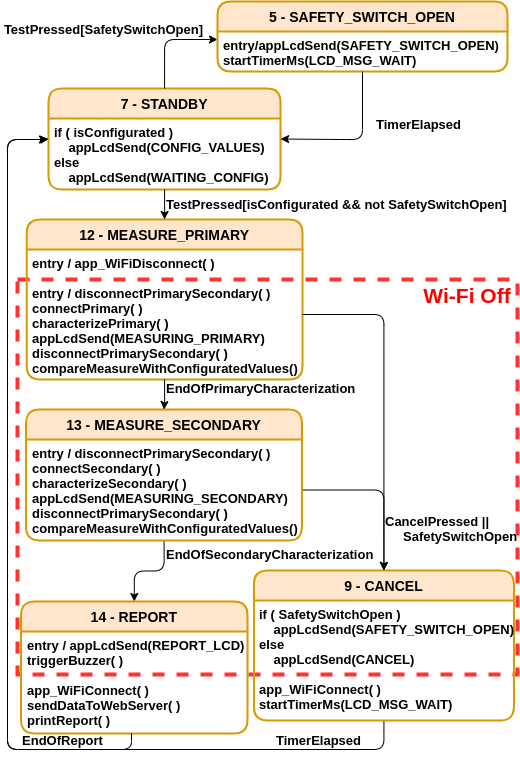
\includegraphics[scale=0.95]{./Figures/MainFSM_3.png}
	\caption{Etapa de caracterización.}
	\label{fig:MainFSM_3}
\end{figure}

Al igual que en la etapa de configuración, en el estado 7 (\textit{STANDBY}) se muestra en el \textit{display} si el equipo fue o no configurado previamente. Se supone que para iniciar la etapa de caracterización el equipo fue configurado, de lo contrario, no se podrá avanzar en la caracterización (estado \textit{NOT\_CONFIGURATED}).

Existen dos caminos posibles en la etapa de caracterización para salir del estado \textit{STANDBY}, ambos son por medio del pulsador Testear, y la diferencia radica en el estado del \textit{switch} de la tapa de seguridad (\textit{SafetySwitchOpen}). Para poder inicializar la caracterización el \textit{switch} debe estar cerrado, en caso contrario el equipo pasa al estado 5 (\textit{SAFETY\_SWITCH\_OPEN}), muestra un mensaje de tapa de seguridad abierta y vuelve al estado \textit{STANDBY}.

Por otro lado, si al pulsar Testear el \textit{switch} se encuentra cerrado, la secuencia de caracterización comenzará normalmente. A continuación se pasa a los estados 12 (\textit{MEASURE\_PRIMARY}) y 13 (\textit{MEASURE\_SECONDARY}). Estos estados fueron simplificados por claridad en la figura. Las principales tareas del estado \textit{MEASURE\_PRIMARY} se detallan a continuación en secuencia:

\begin{enumerate}
\item Desconectar el equipo de la red Wi-Fi.
\item Desenergizar ambos bobinados. Esto se realiza por seguridad ya que, en principio, deberían estar desenergizados.
\item Energizar el bobinado primario.
\item Llamar a las rutinas de medición de valor eficaz para obtener los valores de:
\begin{itemize}
 	\item Tensión en bobinado primario.
	\item Corriente que circula por el bobinado primario.
	\item Tensión en bobinado secundario.
\end{itemize}
\item Mostrar los valores medidos. Esto es opcional, se puede elegir al inicio del sistema.
\item Desenergizar ambos bobinados.
\item Comparar los valores medidos con los umbrales configurados previamente y generar el resultado de las comparaciones.
\end{enumerate}

Al finalizar el estado \textit{MEASURE\_PRIMARY} se pasa al estado \textit{MEASURE\_SECONDARY}. Las principales funciones de este estado se listan a continuación en secuencia:

\begin{enumerate}
\item Desenergizar ambos bobinados. Esto se realiza por seguridad ya que, en principio, deberían estar desenergizados.
\item Energizar el bobinado secundario.
\item Llamar a las rutinas de medición de valor eficaz para obtener los valores de:
\begin{itemize}
 	\item Tensión en bobinado primario.
	\item Tensión en bobinado secundario.
	\item Corriente que circula por el bobinado secundario.	
\end{itemize}
\item Mostrar los valores medidos. Esto es opcional, se puede elegir al inicio del sistema.
\item Desenergizar ambos bobinados.
\item Comparar los valores medidos con los umbrales configurados previamente y generar el resultado de las comparaciones.
\end{enumerate}

Al finalizar los estados \textit{MEASURE\_PRIMARY} y \textit{MEASURE\_SECONDARY}, se cuenta con el resultado de la caracterización, solo resta la etapa de reporte cuyo estado principal es el estado 14 (\textit{REPORT}). 

Como se puede observar en la figura \ref{fig:MainFSM_3} y en los pasos descritos, la comunicación Wi-Fi se detiene en el momento de realizar la medición de los valores eficaces. De los ensayos realizados con el equipo, se pudo notar que, al medir con la comunicación Wi-Fi encendida, las mediciones no resultaban estables e inclusive se observaba un desplazamiento en ellas. Esto es un efecto que fue anticipado en el análisis de riesgo realizado en el plan de proyecto. Este inconveniente, introducido por el periférico Wi-Fi en las mediciones, fue subsanado al apagar el periférico mientras se mide y encenderlo al finalizar esta tarea.

Por último, el proceso de caracterización puede ser cancelado por dos motivos: 
\begin{itemize}
 	\item Pulsar el pulsador Cancelar (\textit{CancelPressed}).
	\item Si la tapa de seguridad se abre (\textit{SafetySwitchOpen}).	
\end{itemize}
Al cancelar la caracterización se pasa al estado 9 (\textit{CANCEL}) y finalmente al estado \textit{STANDBY}.

\subsubsection{Etapa de reporte}
\label{subsubsec:EtRep}

En la figura \ref{fig:MainFSM_4} se muestra la sub-máquina de estado correspondiente a la etapa de reporte. 

\begin{figure}[htpb]
	\centering
	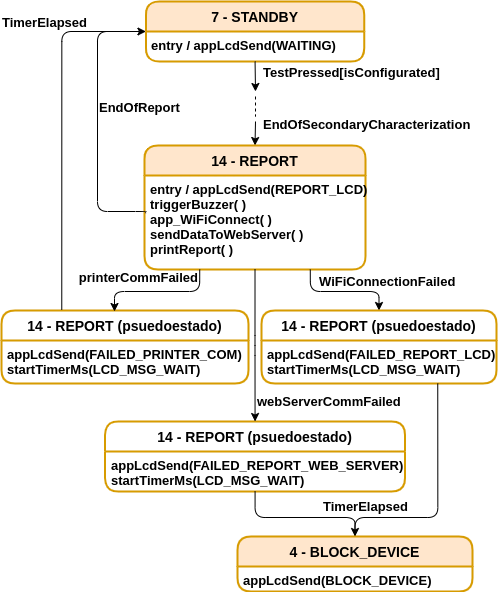
\includegraphics[scale=1]{./Figures/MainFSM_4.png}
	\caption{Etapa de reporte.}
	\label{fig:MainFSM_4}
\end{figure}

Al finalizar los estados \textit{MEASURE\_PRIMARY} y \textit{MEASURE\_SECONDARY} se pasa al estado 14 (\textit{REPORT}), el cual constituye la etapa de reporte.

Dentro de la etapa de reporte se realizan las siguientes acciones:
\begin{itemize}
\item Mostrar el resultado del ensayo en el \textit{display}.
\item Accionar el \textit{buzzer} adecuadamente según el resultado.
\item Reconectar a la red Wi-Fi.
\item Enviar los resultados y los valores medidos al servidor web.
\item Imprimir la etiqueta con los resultados y los valores medidos.
\end{itemize}

En el caso que alguno de los pasos anteriores fallen, se transiciona a un pseudoestado dentro del estado \textit{REPORT} y se muestra la falla en el \textit{display}. En caso de ser una falla grave, que impide la comunicación de resultados al servidor web, se transiciona al estado \textit{BLOCK\_DEVICE}.

\subsection{Medición de valor eficaz}
\label{subsec:RMS}

Los monitores de tensión y corriente alterna del bobinado primario y secundario son los bloques encargados de entregarle al controlador principal los valores RMS de dichas variables. Para tal fin, las salidas de los sensores de tensión y corriente presentados en las secciones \ref{sec:secZMPT101B} y \ref{sec:secZMCT103C}, luego de pasar por un divisor resistivo acorde y un filtro pasa bajos (RC), son conectadas a cuatro canales del ADC1 del módulo ESP32-WROOM-32 como se muestra en la tabla \ref{tab:diagramaPines}.

Las rutinas encargadas de leer los valores de los canales del ADC1 y retornar dichos valores eficaces se encuentran en el archivo adc.h. En el código \ref{cod:adc_h} se muestra el archivo de cabecera simplificado. 

\begin{lstlisting}[label=cod:adc_h,caption=Pseudocódigo del módulo adc.h.] % Start your code-block

/**
 * @brief Initialize ADC 
 * 
 */
void appAdcInit(void);

/**
 * @brief Start a new RMS ADC conversion
 * 
 * @param rms
 *
 * @note This function takes about 1.6 seg in processing the four ADC channels
 *       It reads AMOUNT_OF_CYLCES cycles sampling SAMPLES_IN_20MS in 20 ms for each channel
 */
void appAdcStart(rms_t *rms);

\end{lstlisting}

En el archivo se definen dos funciones:
\begin{itemize}
\item appAdcInit que se utiliza para inicializar todo el hardware necesario para el uso del conversor analógico-digital.
\item appAdcStart que es llamada desde el controlador principal cada vez que se desea iniciar una conversión. Esta función acepta un puntero a la estructura rms\_t para devolver los valores leídos. 
\end{itemize}

Un detalle, a destacar en el código mostrado, es que las funciones presentadas se documentaron por medio de Doxygen, esto es algo que se puede ver en los diferentes archivos de cabecera que se muestran a lo largo de la memoria.

En el pseudocódigo mostrado en el código \ref{cod:adc_c} se muestra la implementación de la función appAdcStart. Esta función utiliza los siguientes módulos del entorno de desarrollo ESP-IDF presentados en la sección \ref{sec:ESPIDF}: 
\begin{itemize}
\item Conversor analógico-digital \citep{ADC}.
\item \textit{Inter-IC Sound} (I2S): que configurado en el modo ADC/DAC proporciona un periférico DMA para ser usado con el ADC y/o DAC \citep{I2S}.
\end{itemize}

El código presentado está simplificado para mostrar su operación, pero cabe destacar que, además de lo mostrado en el código \ref{cod:adc_c}, se utilizaron diferentes herramientas de FreeRTOS en la la función appAdcStart. Las colas para sincronizar el funcionamiento del DMA con el resto de la función son un ejemplo de ello.

\begin{lstlisting}[label=cod:adc_c,caption=Pseudocódigo del módulo adc.c.]

static adc_t adc[ADC_CHANNELS];

void appAdcStart(rms_t *rms) {
	int32_t s_rms;
	
	// Habilitación del DMA 
	i2s_adc_enable(I2S_NUM_0);

	// Barrido de los 4 canales del ADC1
	for (adcIndex=0; adcIndex<ADC_CHANNELS-1; adcIndex++) {		
		// Lectura del canal propiamente dicha
		i2s_read(I2S_NUM_0, buffer);
		
		// Filtro digital de primer orden
		firstOrderFilter(buffer);

		// Cálculo de valor eficaz
		adc[adcIndex].rms = getRMS(buffer);
		
		// Calibración de la entrada 
		calibration(&adc[adcIndex].rms,  adc[adcIndex].offset, adc[adcIndex].gain);
		
		// Cambiar el canal a medir del ADC1
		i2s_set_adc_mode(ADC_UNIT_1, adc[adcIndex].channel);
	}
	
	// Deshabilitar el DMA
	i2s_adc_disable(I2S_NUM_0);
}
\end{lstlisting}

Al ingresar a la función appAdcStart se habilita el DMA por medio de la función i2s\_adc\_enable. El próximo paso es barrer los cuatro canales del ADC1 para la cual se utiliza un lazo de tipo \textit{for}. Dentro del lazo, la función i2s\_read muestrea el canal del ADC1 seleccionado. Dicha función fue configurada para leer 8 ciclos de la señal de entrada y tomar 128 muestras por cada ciclo, hasta que se realiza esta acción la función permanece bloqueada. Como se miden las variables de la red de energía eléctrica, su periodo es de 20 ms, lo que da un tiempo de medición por canal de 160 ms, ecuación \ref{eq:TMED}.

\begin{equation}
	\label{eq:TMED}
	T_{MED} = 8 * 20 ms = 160 ms
\end{equation}

Y se obtienen 1024 muestras por canal, ecuación \ref{eq:puntos}.

\begin{equation}
	\label{eq:puntos}
	N = 8 * 128 = 1024
\end{equation}

Por lo tanto, la función i2s\_read permanece bloqueada durante 160 ms y devuelve un puntero a un vector con 1024 puntos de la señal de entrada. Este vector es luego filtrado con un filtro digital de primer orden cuya estructura se muestra en la ecuación \ref{eq:filtro}. Los valores de A$_{1}$ y B$_{0}$ se ajustaron convenientemente en función de la frecuencia de muestreo del sistema y la respuesta deseada del filtro.

\begin{equation}
	\label{eq:filtro}
	y\left( n \right) = A_1 y\left( n-1 \right) + B_0 x\left( n \right)
\end{equation}

Luego del filtrado, se procede a calcular el valor eficaz de los valores medidos por medio de la función getRMS. Se utilizó la ecuación \ref{eq:RMS} para el cálculo del valor eficaz de las muestras obtenidas, donde CICLOS=8 y N$_{CICLOS}$=128. Con el filtro digital y el promedio de 8 ciclos de la señal medida se obtiene un valor estable y ayuda a lidiar con las conexiones de la placa universal y las salidas de los módulos sensores.

\begin{equation}
	\label{eq:RMS}
rms=\frac{1}{CICLOS}\sum_{n=0}^{CICLOS-1}\sqrt{\frac{1}{N_{CICLOS}}\sum_{i=0}^{ N_{CICLOS}-1} buffer\left [ n \right ]\left [ i \right ]*buffer\left [ n \right ]\left [ i \right ]}
\end{equation}

Finalmente, se realiza una corrección lineal del valor obtenido, función calibration en el código, a partir de un desplazamiento (\textit{offset}) y una ganancia (\textit{gain}) preconfigurados. Se puede observar que cada uno de los pasos mencionados se realiza sobre cada canal independientemente, puntualmente la calibración de las señales, para la cual se cuenta con un juego de ganancias y desplazamientos independientes para cada canal.

\subsection{Comunicación Wi-Fi}

El módulo de comunicación Wi-Fi es el módulo más complejo del sistema. Este, no solo debe ser capaz de controlar la configuración, conexión y desconexión del módulo a la red Wi-Fi, sino que, además, debe leer y escribir a memoria no volátil las credenciales de la red Wi-Fi y manejar el protocolo SmartConfig. 

En la figura \ref{fig:WiFi} se muestra un diagrama de flujo simplificado de las etapas seguidas para la gestión de la red Wi-Fi. 

\pagebreak

\begin{figure}[ht]
	\centering
	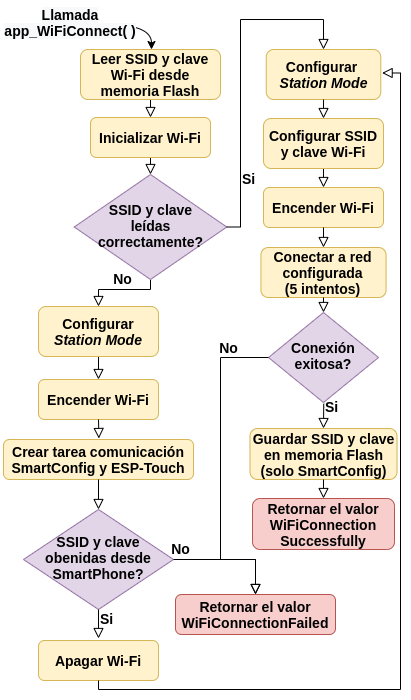
\includegraphics[scale=0.95]{./Figures/WiFi.png}
	\caption{Secuencia de conexión a red Wi-Fi.}
	\label{fig:WiFi}
\end{figure}

Las principales librerías del entorno ESP-IDF utilizadas para el desarrollo de este módulo son: 
\begin{itemize}
\item \textit{Non-volatile storage library} \citep{NVL}: utilizada para leer y escribir las credenciales de Wi-Fi hacia y desde la memoria \textit{flash}. Se tuvo el cuidado de validar los datos leídos para evitar errores en las librerías de Wi-Fi por leer datos corruptos desde la memoria.
\item Wi-Fi \citep{ESPIDF:WiFi}.
\item SmartConfig: utilizado en conjunto con la aplicación móvil ESP-Touch como se explica en la sección \ref{sec:ESPTouch}.
\end{itemize}

Para sincronizar las diferentes tareas se utilizó la librería de eventos \textit{Event Loop Library} \citep{EVENT}, la cual permite pasar por los diferentes estados de la comunicación y evitar condiciones de carrera. Por simplicidad, en el diagrama de flujo de la figura \ref{fig:WiFi} se omiten estos eventos. Sin embargo, en la descripción posterior se nombrarán alguno de ellos para tener una mejor correlación con el trabajo realizado.

Para iniciar la conexión a la red Wi-Fi el controlador principal debe llamar a la función app\_WiFiConnect como se explicó en la sección \ref{subsubsec:EtIni}. Una vez llamada dicha función ocurre la secuencia de la figura \ref{fig:WiFi}. El primer paso es leer la memoria no volátil en busca de las credenciales de Wi-Fi, en caso de obtenerlas sin error, se procede a configurar el periférico en modo estación (\textit{station mode}), configurar las credenciales en una estructura de configuración provista por la librería Wi-Fi y encender el periférico. El próximo paso es esperar por el evento WIFI\_CONNECTED o el evento WIFI\_FAIL. En caso de recibir este último, se reintenta 5 veces para poder conectar, si no se logra se retorna de la función app\_WiFiConnect con el valor \textit{WiFiConnectionFailed}. En caso de obtener el evento  WIFI\_CONNECTED en alguno de los intentos, la función retorna con el valor \textit{WiFiConnectionSuccessfully}.

En caso de no tener las credenciales de Wi-Fi configuradas u obtener un error al intentar leerlas, la función app\_WiFiConnect puede utilizar SmartConfig para intentar adquirirlas desde la aplicación móvil ESP-Touch. Para esto, se crea una tarea de FreeRTOS para utilizar las funciones de la librería de SmartConfig. Dentro de la tarea se espera por el evento ESPTOUCH\_DONE que se genera cuando la aplicación ESP-Touch envía las credenciales. Luego de obtener las credenciales, se procede a intentar conectar nuevamente por medio del procedimiento explicado en el párrafo anterior. La única diferencia en este caso, es que si se logra conectar exitosamente a Wi-Fi, se guardan las nuevas credenciales en memoria no volátil para su posterior reutilización. Por otro lado, la tarea de FreeRTOS creada para administrar el protocolo SmartConfig se borra del sistema al finalizar el procedimiento ya que la acción de generar las credenciales de Wi-Fi es una tarea de un solo uso y carece de sentido tenerla corriendo todo el tiempo.


\subsection{Obtención y envió de datos al webserver}

Como se explicó en los capítulos introductorios, el cliente desarrolló un servidor web donde consultar los valores de comparación de tensiones y corrientes y a donde enviar los valores medidos y los resultados obtenidos. 

La forma de comunicarse con el servidor web es a través de comandos GET y POST de HTTP. Por otro lado, la información a ser transmitida y/o recibida se procesa en el cuerpo de los comandos GET y POST en formato JSON.

Para recibir los datos de configuración se debe enviar el siguiente comando GET:

\begin{table}[htpb]
\centering
\begin{tabular}{|l|}
\hline
\begin{tabular}[c]{@{}l@{}}\textbf{GET} /TransformersTesterConfigs/Last \textbf{http/1.1}\\ \textbf{Host:} https://iris-test-api.azurewebsites.net/api\\ \textbf{Content-Type:} application/json\end{tabular} \\ \hline
\end{tabular}
\end{table}

Y se obtiene una respuesta como la siguiente:

\pagebreak

\begin{table}[htpb]
\centering
\begin{tabular}{|l|}
\hline
\begin{tabular}[c]{@{}l@{}}\textbf{HTTP/1.1 200 OK}\\ \textbf{Content-Type:} application/json\\ \textbf{Server:} Kestrel\end{tabular} \\ \hline
\begin{tabular}[c]{@{}l@{}}\{\\ \hspace{0.6cm}``id'':4,\\ \hspace{0.6cm}``createDate'':``2021-03-10T15:59:04'',\\ \hspace{0.6cm}``code'':``MPELETRAN-0023'',\\ \hspace{0.6cm}``batchId'':``20210310-1'',\\ \hspace{0.6cm}``vinPrimaryMin'':225.00,\\ \hspace{0.6cm}``voutSecondaryMin'':14.00,\\ \hspace{0.6cm}``iPrimaryMin'':15.00,\\ \hspace{0.6cm}``vinSecondaryMin'':14.00,\\ \hspace{0.6cm}``voutPrimaryMin'':210.00,\\ \hspace{0.6cm}``iSecondaryMin'':100.00,\\ \hspace{0.6cm}``vinPrimaryMax'':235.00,\\ \hspace{0.6cm}``voutSecondaryMax'':17.00,\\ \hspace{0.6cm}``iPrimaryMax'':70.00,\\ \hspace{0.6cm}``vinSecondaryMax'':16.00,\\ \hspace{0.6cm}``voutPrimaryMax'':230.00,\\ \hspace{0.6cm}``iSecondaryMax'':400.00\\ \}\end{tabular} \\ \hline
\end{tabular}
\end{table}

A la comunicación con el servidor web y el procesamiento de los paquetes se lo dividió en dos capas de software:
\begin{itemize}
\item Capa HTTP (http\_client.h): encargada de procesar los comandos GET y POST de HTTP.
\item Capa de procesamiento de paquetes (app\_Comm.h): encargada de tomar los datos enviados o recibidos de la capa HTTP y armar o desarmar (``parsear'') los paquetes JSON.
\end{itemize}

Para el desarrollo de la capa HTTP se utilizó la librería cliente HTTP del entorno de desarrollo ESP-IDF \citep{HTTPC}. En el código \ref{cod:http_c} se muestra un pseudocódigo para la función GET, la implementación de la función POST es similar.

\begin{lstlisting}[label=cod:http_c,caption=Pseudocódigo función GET de HTTP.]
#include "esp_http_client.h"

#define GET_URL   "https://iris-test-api.azurewebsites.net/api/TransformersTesterConfigs/Last"

esp_err_t get_http_config(char *buffer)
{
    esp_http_client_config_t config = {
    	.url = GET_URL,
    };

    // Inicializar el cliente HTTP
    esp_http_client_init(&config);
    
    // Abrir conexión con el servidor
    if ((err = esp_http_client_open(client, 0)) != ESP_OK) {
        return (err);
    }
    
    // Armar encabezado método GET
    esp_http_client_set_method(client, HTTP_METHOD_GET);
    esp_http_client_set_header(client, "Content-Type", "application/json");
    
    // Enviar paquete GET y capturar respuesta
    read_len = esp_http_client_read(client, buffer, BUFFER_SIZE);
    if (read_len <= 0) {
        return (ESP_FAIL);
    }
    
    // Cerrar la conexión con el cliente HTTP
    esp_http_client_close(client);

    return (err);
}

\end{lstlisting}

En el caso de un comando GET, los datos recibidos desde la capa HTTP son luego pasados a la capa de procesamiento de paquetes donde se procede a ``parsearlos'' y validarlos. Entre las rutinas de validación, se encuentra el chequeo de los datos numéricos. En la capa de procesamiento, los datos se guardan en una estructura de tipo configData\_t diseñada para tal fin. La estructura configData\_t permite el fácil acceso de los datos obtenidos del servidor web por parte del controlador principal. En el código \ref{cod:struct_http} se muestra la jerarquía de estructuras desarrollada para la estructura configData\_t, aquí también se puede apreciar que está documentada con Doxygen.

\begin{lstlisting}[label=cod:struct_http,caption=Estructuras para el manejo de los datos recibidos.]
/**
 * @brief Parameter thresholds structure
 *
 */
typedef struct {
	int32_t max;
	int32_t min;
} parametersRange_t;

/**
 * @brief Measured Parameters structure
 *
 */
typedef struct {
	parametersRange_t Vinp;   /*!<Primary Voltage    */
	parametersRange_t Voutp;  /*!<Primary Voltage    */
	parametersRange_t Vins;   /*!<Secondary Voltage  */
	parametersRange_t Vouts;  /*!<Secondary Voltage  */
	parametersRange_t Ip;     /*!<Primary current    */
	parametersRange_t Is;     /*!<Secondary current  */
} trafoParameters_t;

/**
 * @brief Configuration data type
 *
 */
typedef struct {
	uint32_t id;                      /*!<Test Identification Number   */
	char batchId[BATCHID_LENGTH];     /*!<Transformer BatchId          */
	char code[CODE_LENGTH];           /*!<Transformer code             */
	trafoParameters_t trafoParameters;/*!<Measured Parameters structure*/
} configData_t;
\end{lstlisting}


\subsection{Implementación del protocolo DPL}

Entre las tareas que el controlador principal debe realizar en la etapa de reporte (sección \ref{subsubsec:EtRep}) se encuentra la impresión de una etiqueta con los resultados del ensayo. Para ello, se utilizó la impresora presentada en la sección \ref{sec:Impre} cuyo protocolo se conoce como DPL y fue introducido en la misma sección. En esta sección se explica la implementación de dicho protocolo.

El protocolo DPL fue implementado en el módulo app\_printer.c, en tanto que, la capa física del protocolo fue resuelta con el módulo de hardware presentado en la sección \ref{fig:rs232}. Para su manejo se utilizó la librería UART que se encuentra dentro de los controladores de periféricos provisto por el entorno ESP-IDF \citep{ESPIDF:PER}.

Cuando el controlador principal desea imprimir los resultados del ensayo debe llamar a la función \textit{print}. Esta función implementa todos los comandos necesarios para utilizar el protocolo DPL y devuelve el resultado de la impresión. En el código \ref{cod:print_h} se muestran los valores devueltos por la función \textit{print}.

 \begin{lstlisting}[label=cod:print_h,caption=Prototipo función print.]
/**
 * @brief Printer status
 * 
 */
typedef enum {
	PRINTER_NO_COMM,   /*!<Printer never respond             */
	PRINTER_NOT_READY, /*!<Printer is not ready, answer to 
	                       command <SOH>A/r (Status request) */
	PRINTER_READY,     /*!<Printer ready to print            */
	PRINTER_OK         /*!<The print command was successful  */
} printerStatus_t;
\end{lstlisting}

En la figura \ref{fig:printFunc} se muestra el diagrama de flujo de la función \textit{print}. Los comandos a enviar y la respuesta de la impresora se resaltan en color azul, mientras que el contenido de la etiqueta (resultado obtenido del ensayo y valores medidos) se resalta en verde.

La primera acción a realizar al llamar la función \textit{print} es verificar el estado de la impresora. Para ello, se envía el comando inmediato \textless{}SOH\textgreater{}A\textless{}CR\textgreater{} y a su vez se dispara un temporizador de espera (\textit{timeout}). Si el temporizador de espera llega a su valor de temporización antes que la impresora haya respondido, la función retorna un error de comunicación con la impresora (PRINTER\_NO\_COMM). En caso contrario, la obtención una respuesta, esta es analizada y si es igual a la cadena ``YYYYYYYY\textless{}CR\textgreater{}'' significa que la impresora está en condiciones de imprimir. Por otro lado, en caso de recibir algún carácter 'N' dentro de la trama anterior, significa que la impresora no está disponible y se retorna de la función \textit{print} con un estado de error PRINTER\_NOT\_READY.

En caso que la impresora esté en condiciones de imprimir (PRINTER\_READY), se pasa a enviar el comando \textless{}STX\textgreater{}L\textless{}CR\textgreater{} para iniciar la impresión de la etiqueta propiamente dicha. Después de este, se envían los siguientes comandos de configuración propios de la etiqueta en cuestión:
\begin{itemize}
\item m\textless{}CR\textgreater{}: indica que la etiqueta utiliza unidades internacionales.
\item H15\textless{}CR\textgreater{}: fija la temperatura del cabezal de impresión.
\item D11\textless{}CR\textgreater{}: fija el tamaño del punto de impresión.
\end{itemize}

\pagebreak

\begin{figure}[htpb]
	\centering
	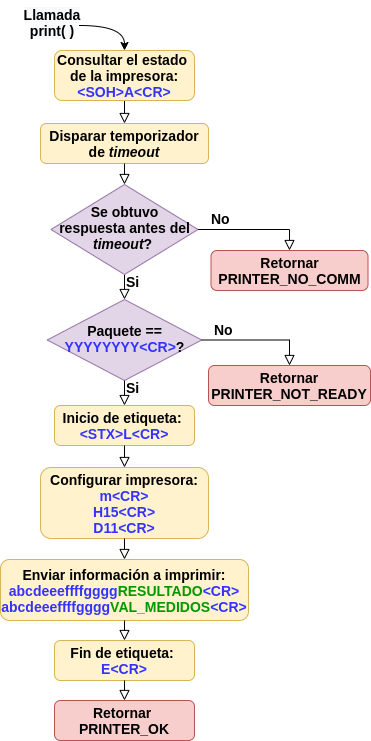
\includegraphics[scale=0.95]{./Figures/printer.png}
	\caption{Diagrama de flujo función de la \textit{print}.}
	\label{fig:printFunc}
\end{figure}

Una vez configurada la impresora para la etiqueta en particular, se procede a enviar la información a imprimir por medio del formato presentado en la tabla \ref{tab:printercmdSystem}. En la figura se indican genéricamente los caracteres ``abcdeeeffffgggg'' ya que estos dependen de cada línea que se quiera imprimir (rotación del texto, tipo de fuente, ubicación del texto, etc). En la misma línea y luego de las caracteres mencionados, se encuentra el dato a imprimir que depende del ensayo (RESULTADO y VAL\_MEDIDOS).

Por último, se envía el comando E\textless{}CR\textgreater{} que le indica a la impresora que se finalizó la carga de la etiqueta y se puede proceder a su impresión. Si se llega al final de este proceso la función \textit{print} devuelve PRINTER\_OK que significa que se pudo imprimir con éxito.

\subsection{Interfaz de usuario}

La interfaz local de usuario está formada por los siguientes elementos:
\begin{itemize}
\item Pulsadores Testear, Configurar y Cancelar.
\item \textit{Buzzer}.
\item \textit{Display} alfanumérico de 20 caracteres por 4 líneas.
\end{itemize}

Para trabajar con todos estos módulos se utilizó la librerías GPIO que se encuentra dentro de los controladores de periféricos provisto por el entorno ESP-IDF \citep{ESPIDF:PER}.

Para el procesamiento de los pulsadores se desarrolló una función para cada uno. Estas funciones deben ser encuestadas (\textit{pulling}) periódicamente para saber el estado de los pulsadores, en el código \ref{cod:app_gpio_h} se muestra el prototipo para el pulsador Cancelar. Adicionalmente, se incorporaron rutinas antirebote (\textit{debouncing}) para todos los pulsadores.

\begin{lstlisting}[label=cod:app_gpio_h,caption=Pseudocódigo del módulo adc.c.]
/**
 * @brief Check if the cancel button was pressed
 * 
 * @return true 
 * @return false 
 */
bool isCancelPressed( void );
\end{lstlisting}

En caso del accionamiento del \textit{buzzer} se debieron generar 2 secuencias según el requerimiento 3 de la sección \ref{subsec:ReqUsu}, para lo cual se utilizó un temporizador de hardware. Para la implementación del temporizador se usó la librería de temporizadores provista por el entorno ESP-IDF dentro de los controladores de periféricos \citep{ESPIDF:PER}.

Por último, para el \textit{display} se tomó como base la librería sAPI \citep{sAPI} que posee un módulo de software para utilizar el controlador HD44780. El código debió ser portado para funcionar en el entorno ESP-IDF. Además del trabajo anterior, se trabajó en mejorar la librería de la sAPI por medio del agregado de varias estructuras de software que permiten inicializar el controlador del \textit{display} de una manera más eficiente.


% Chapter Template

\chapter{Ensayos y resultados} % Main chapter title

\label{Chapter4} % Change X to a consecutive number; for referencing this chapter elsewhere, use \ref{ChapterX}

En este capítulo se presentan los ensayos realizados al trabajo y los resultados obtenidos. Inicialmente, se introducen los ensayos realizados sobre el hardware con un mínimo de bloques de software. Luego, se detallan diferentes ensayos de integración a través del uso de técnicas de \textit{testing} de máquinas de estados finitos.

%----------------------------------------------------------------------------------------
%	SECTION 1
%----------------------------------------------------------------------------------------

\section{Pruebas funcionales de hardware}
\label{sec:pruebasHW}

Las pruebas de hardware se dividieron en tres etapas:

\begin{enumerate}
\item Ensayos sobre \textit{protoboard}. 
\item Primer ensayo de integración, donde los módulos fueron montados sobre una base de madera. 
\item Ensayo final de integración con los elementos montados en los gabinetes.
\end{enumerate}

En la figura \ref{fig:Protoboard} se muestra el banco de pruebas para el sensor de tensión, el \textit{display} y el módulo RS-232 utilizados en los ensayos sobre \textit{protoboard}.

\begin{figure}[htpb]
	\centering
	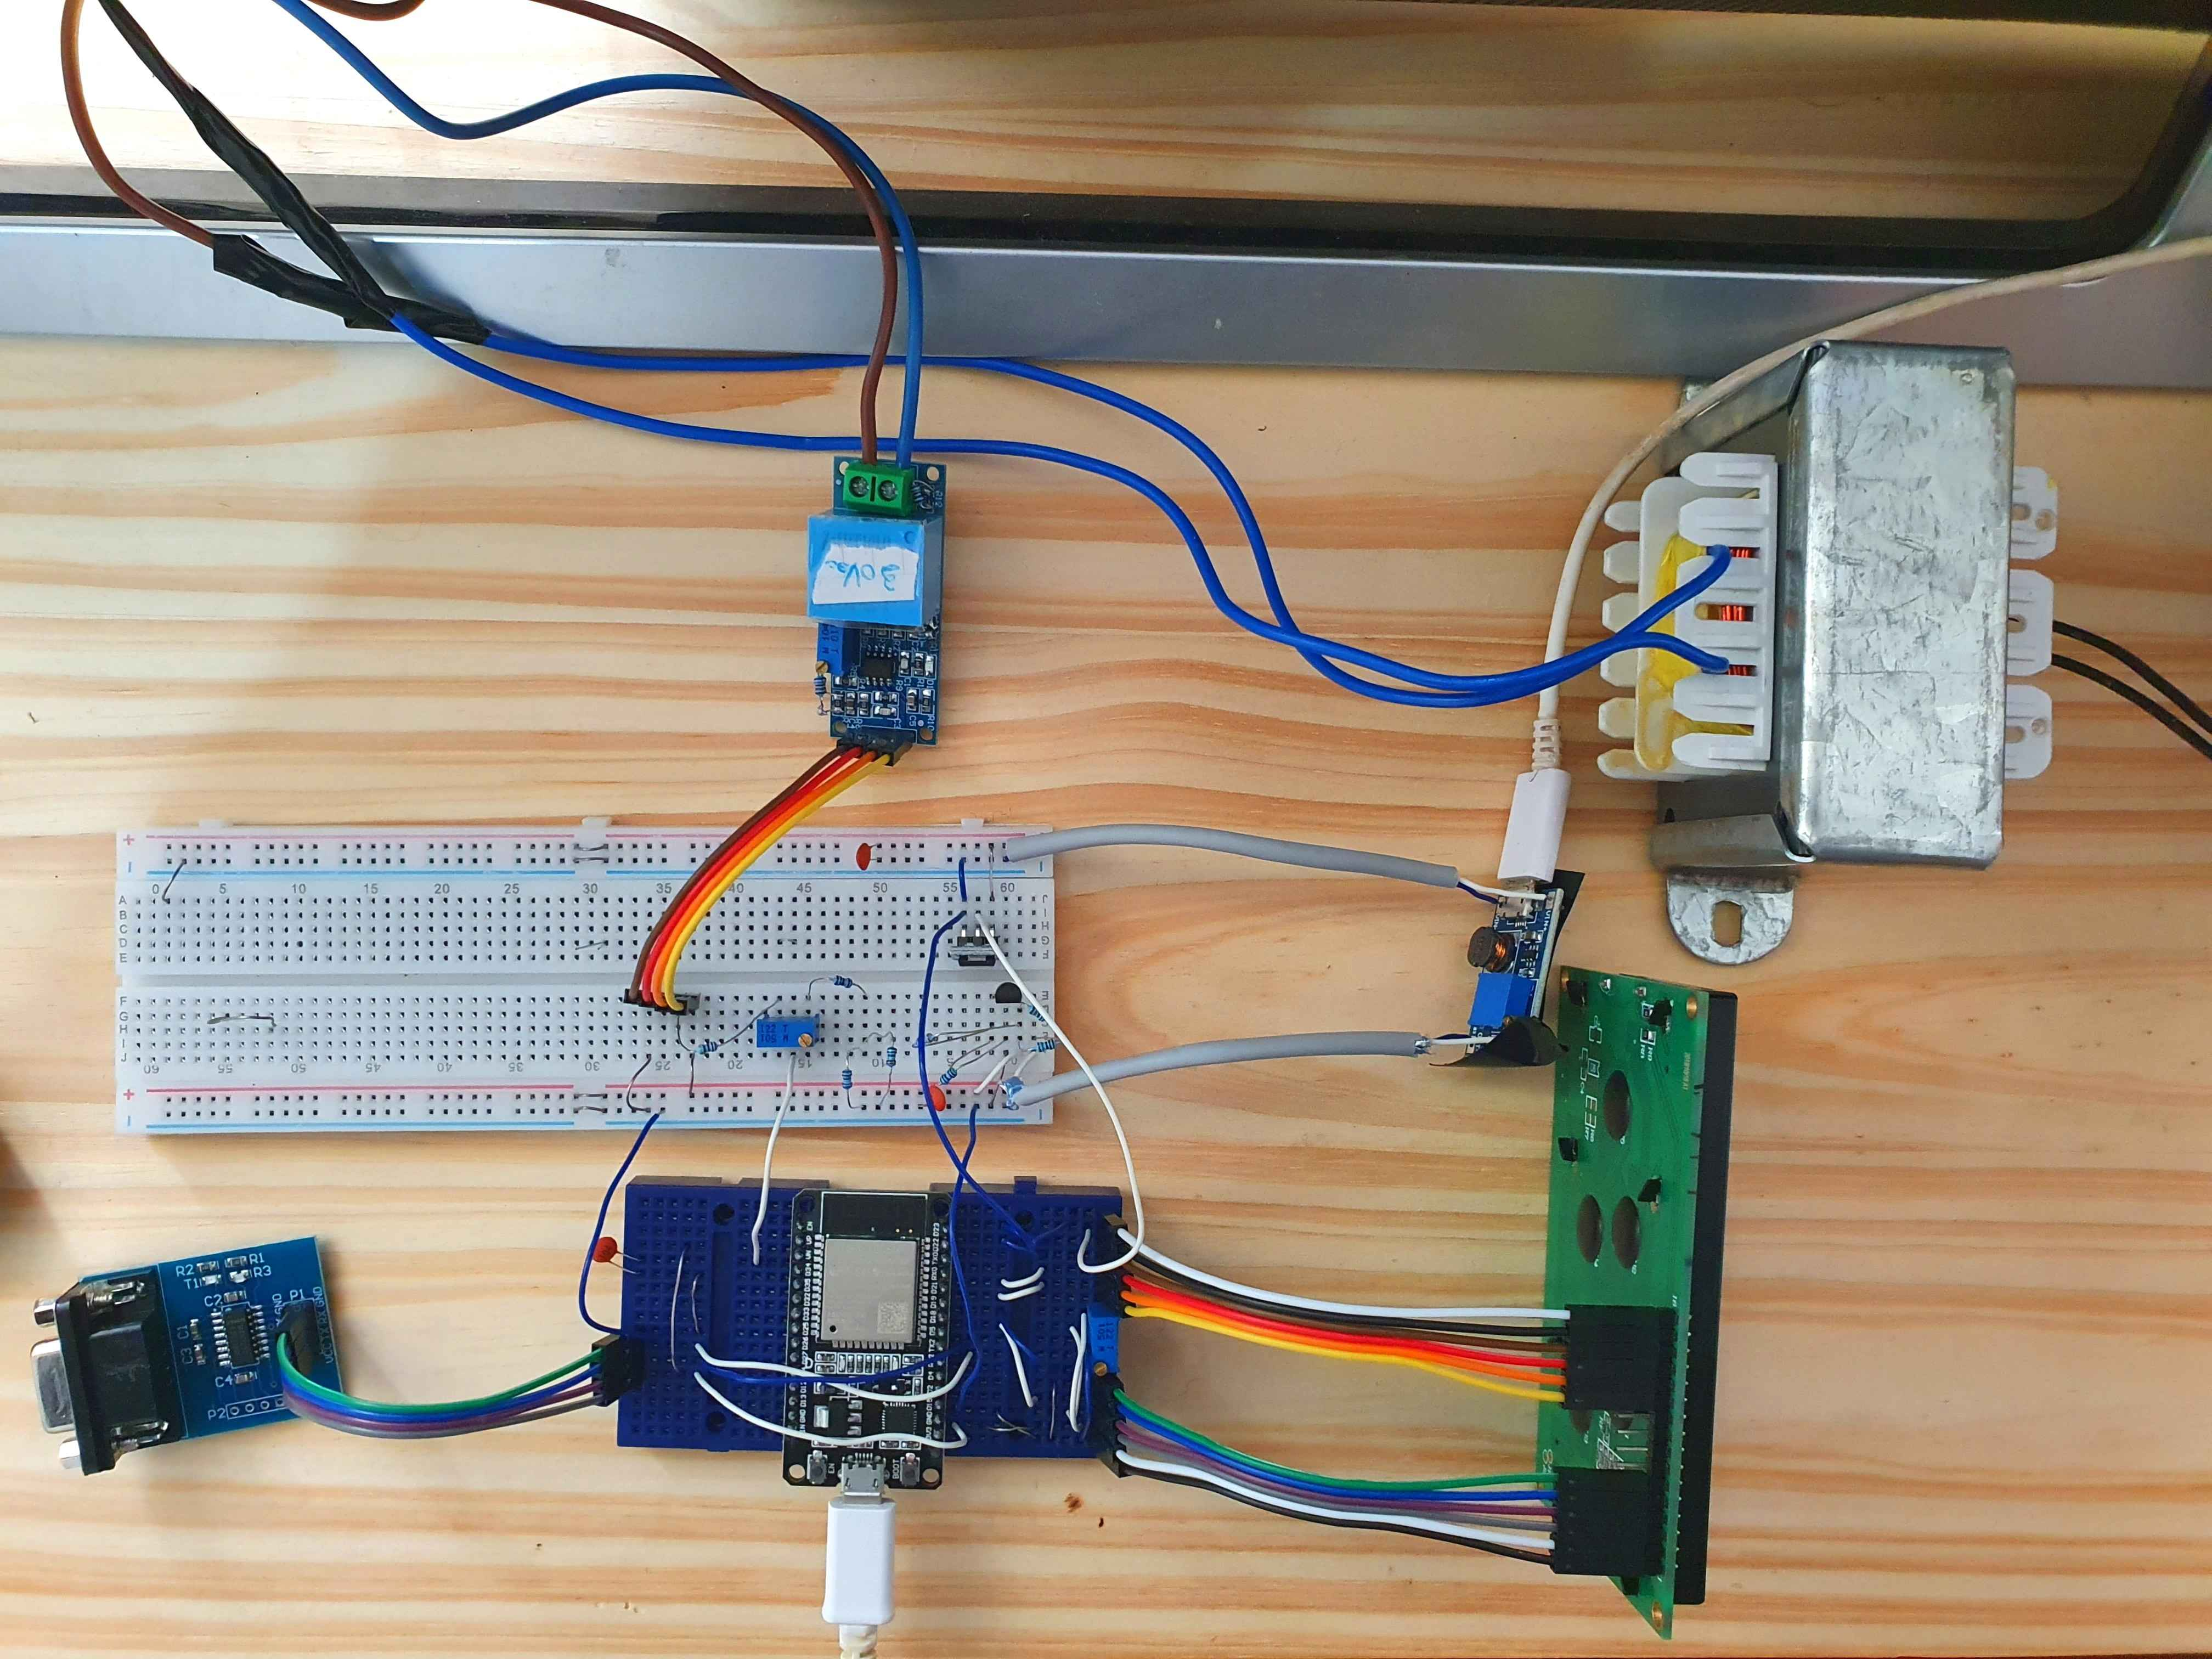
\includegraphics[scale=0.09]{./Figures/protoboard.jpg}
	\caption{Ensayos sobre \textit{protoboard}.}
	\label{fig:Protoboard}
\end{figure}

En los ensayos sobre \textit{protoboard}, se realizaron pruebas sobre los módulos individuales con bloques de firmware reducidos. Las pruebas principales se detallan a continuación:
\begin{enumerate}
	\item Pruebas de los módulos sensores de tensión y corriente.
	\item Pruebas del \textit{display}.
	\item Pruebas sobre la interfaz RS-232 utilizando un terminal.
\end{enumerate}

Para las pruebas sobre los módulos sensores de tensión y corriente se utilizaron los siguientes instrumentos:
\begin{itemize}
\item Multímetro. Marca: Pro'sKit, modelo: MT-1232 \citep{MT1232}.
\item Osciloscopio. Marca: OWON, modelo: VDS3102  \citep{VDS3102}.
\end{itemize}

A partir de estos instrumentos, se realizaron mediciones para constatar la exactitud y repetitividad de los módulos sensores, así como, para ajustar los potenciometros y entregar tensiones acorde para las entradas del ADC del microcontrolador. A modo de ejemplo, en la figura \ref{fig:ISOsc}, se muestra una captura de pantalla de la tensión entregada por el módulo sensor de corriente para el bobinado secundario.

\begin{figure}[htpb]
	\centering
	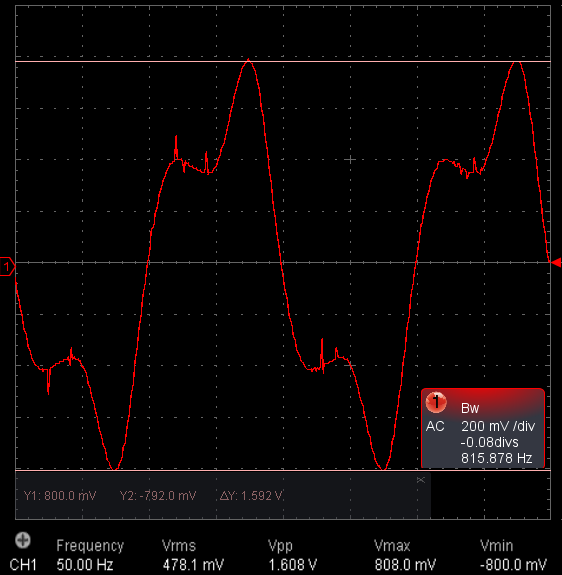
\includegraphics[scale=0.6]{./Figures/osc_is.png}
	\caption{Medición de corriente en el bobinado secundario.}
	\label{fig:ISOsc}
\end{figure}

Luego de validar los módulos de hardware individualmente sobre el \textit{protoboard}, se procedió a montarlos sobre una base de madera y a construir la placa universal. Esta nueva etapa permitió comenzar a trabajar en las pruebas de integración sin necesidad de contar con los gabinetes totalmente ensamblados. Se decidió realizar esta etapa intermedia porque los ensayos en \textit{protoboard} no eran aptos para la gran cantidad de módulos a conectar y, además, representaba un riesgo grande ya que varios módulos están conectados a 220 V$_{RMS}$. En la figura \ref{fig:BaseMadera}, se observa la base de madera con varios módulos montados sobre ella.

\begin{figure}[htpb]
	\centering
	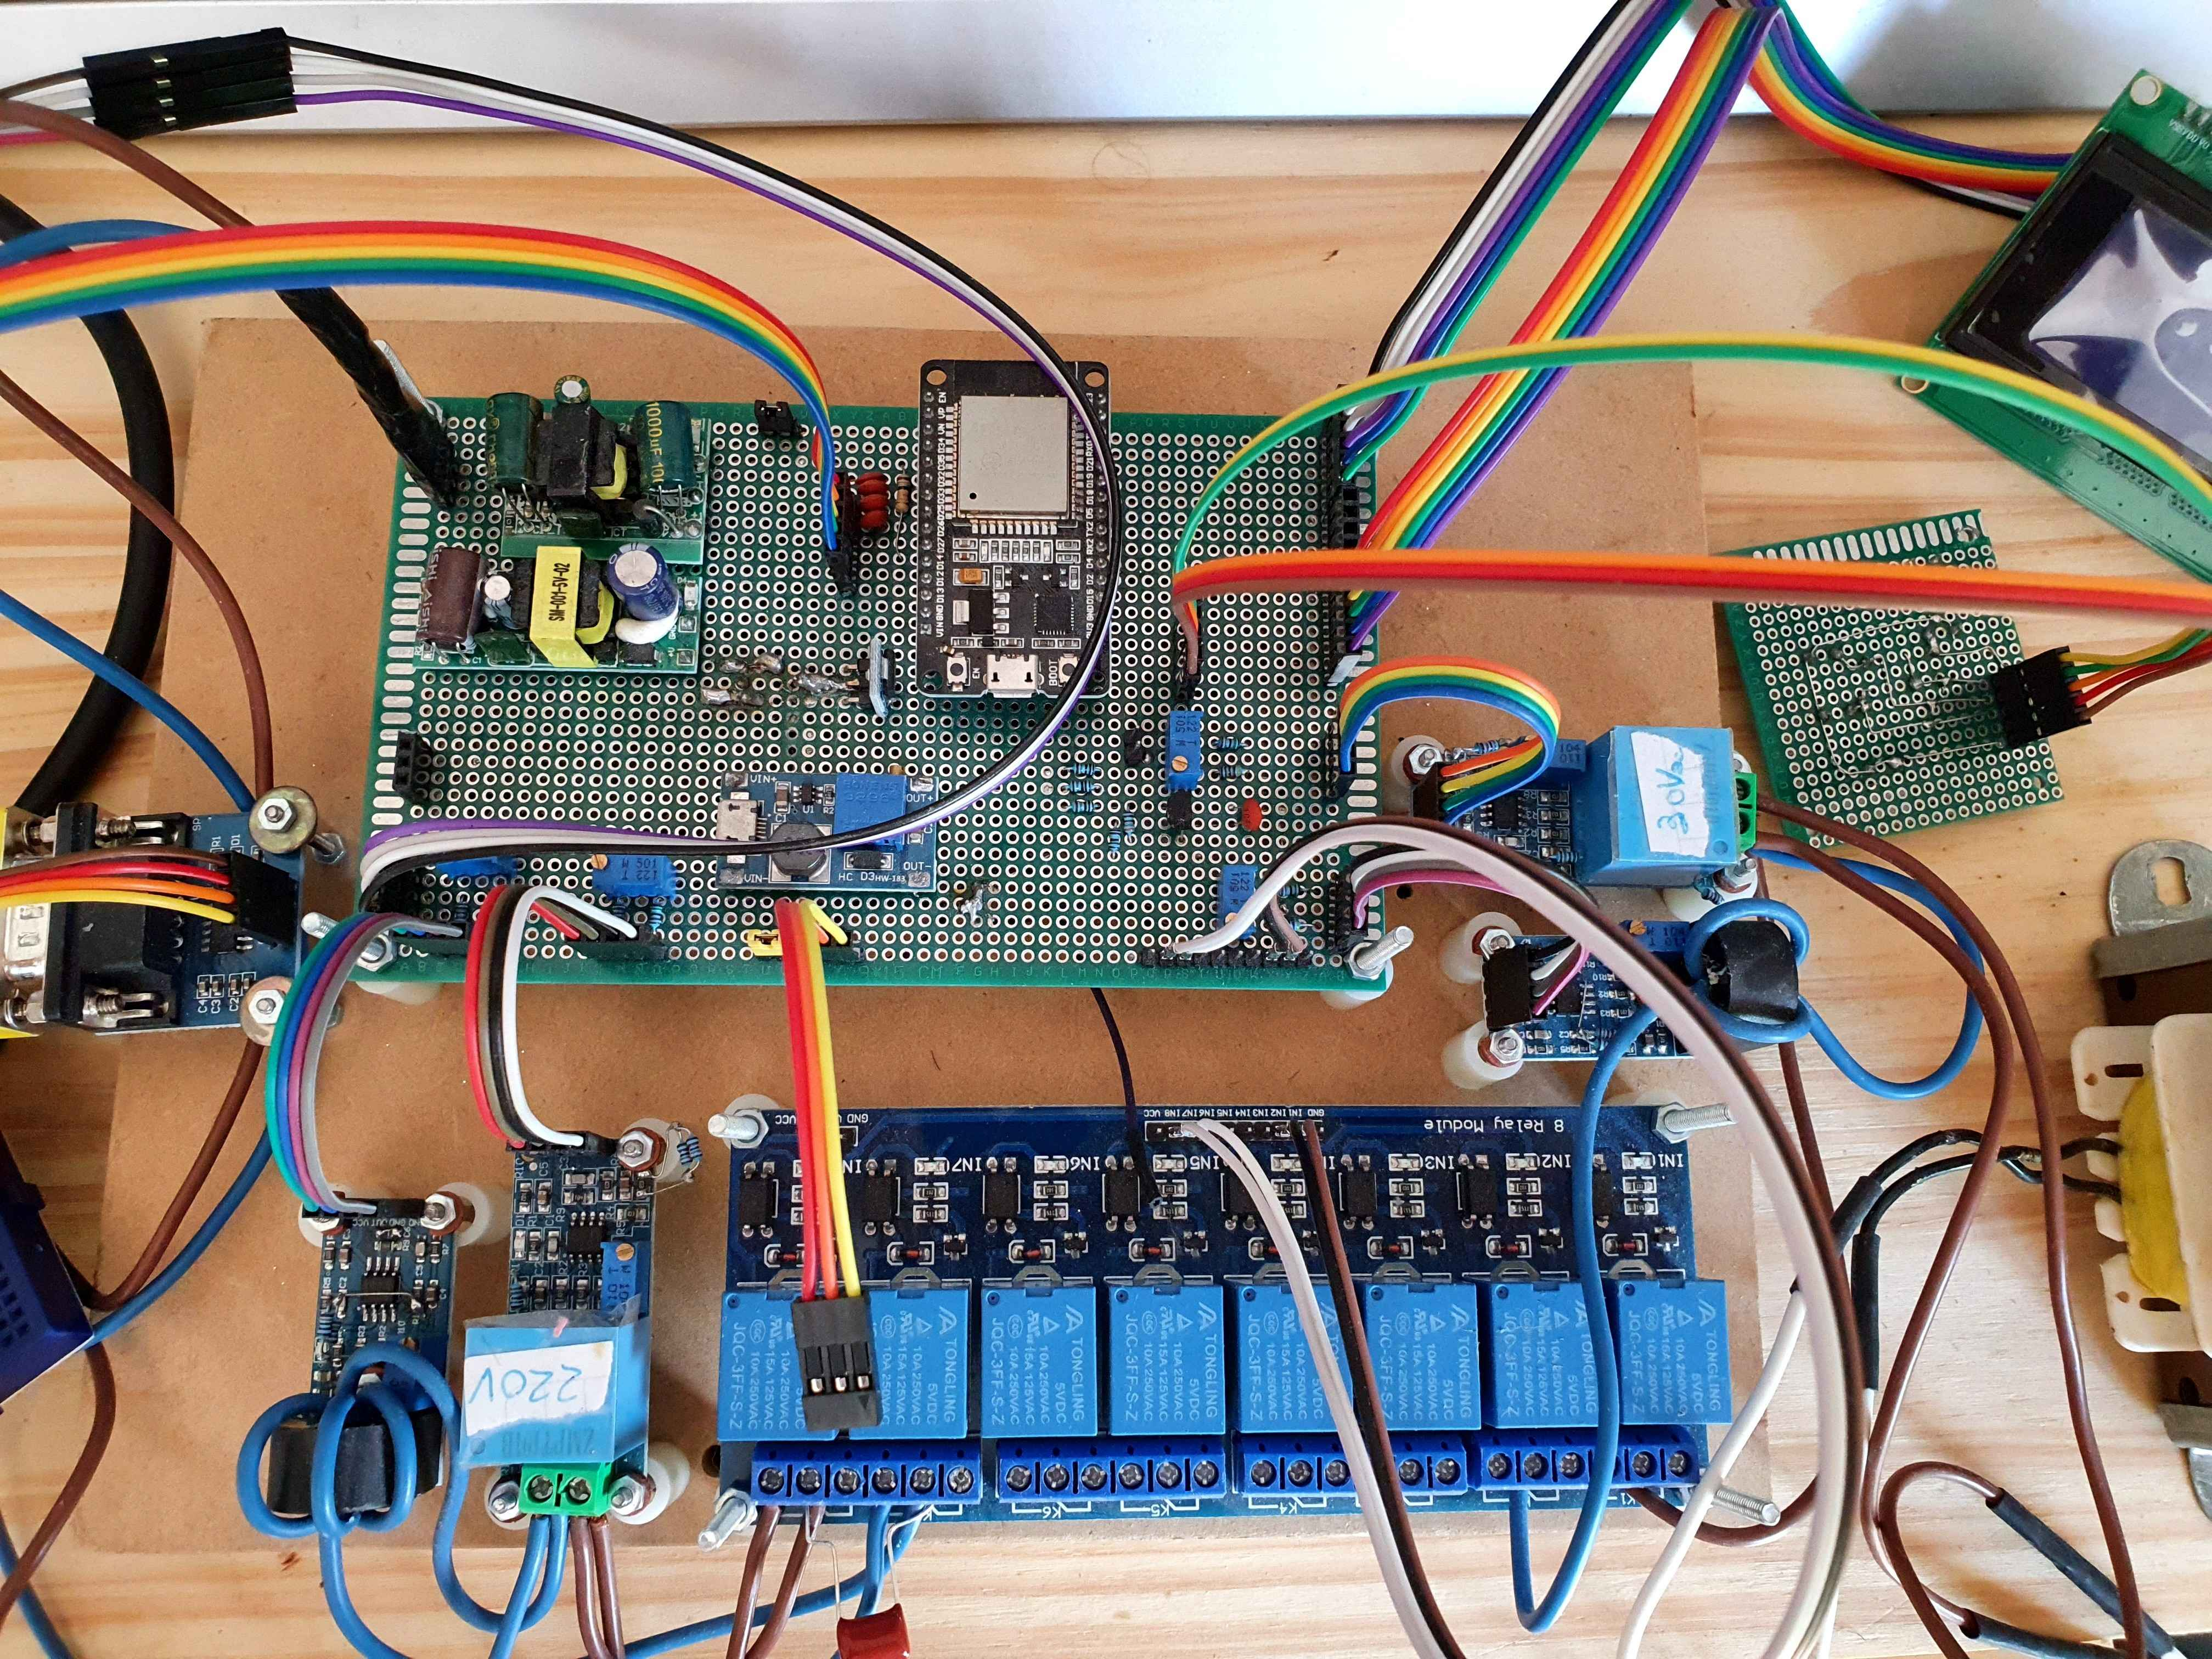
\includegraphics[scale=0.09]{./Figures/madera.jpg}
	\caption{Primera prueba de integración.}
	\label{fig:BaseMadera}
\end{figure}

En esta etapa se realizaron las siguientes pruebas:
\begin{enumerate}
	\item Pruebas del módulo Wi-Fi. Se armaron rutinas básicas de conexión y desconexión y, a través de un \textit{ping} a la IP obtenida por el módulo, se verificó la correcta operación.
	\item Pruebas de las mediciones analógicas. Con la inclusión de la placa universal como interfaz entre los módulos sensores y el kit, se procedió a verificar la lectura de los ADCs dentro del kit.
	\item Pruebas con una impresora de un modelo similar a la adquirida finalmente. Esta impresora fue prestada por el cliente para comprobar la factibilidad de la implementación del protocolo DPL.
\end{enumerate}

Con respecto a las entradas analógicas, se verificó que el período de muestreo fijado sea el esperado. Luego, se evalúo el ruido de la señal digitalizada y se decidió implementar el filtro digital explicado en la sección \ref{subsec:RMS}. Para verificar el filtrado, se procedió a leer el \textit{buffer} de 1024 muestras obtenido del DMA y a leer el mismo \textit{buffer} luego de pasarlo por el filtro digital. En la figura \ref{fig:filtroPrue} se muestra la señal antes y después del filtro y se aprecia la mejora debido al filtrado.

\begin{figure}[htpb]
	\centering
	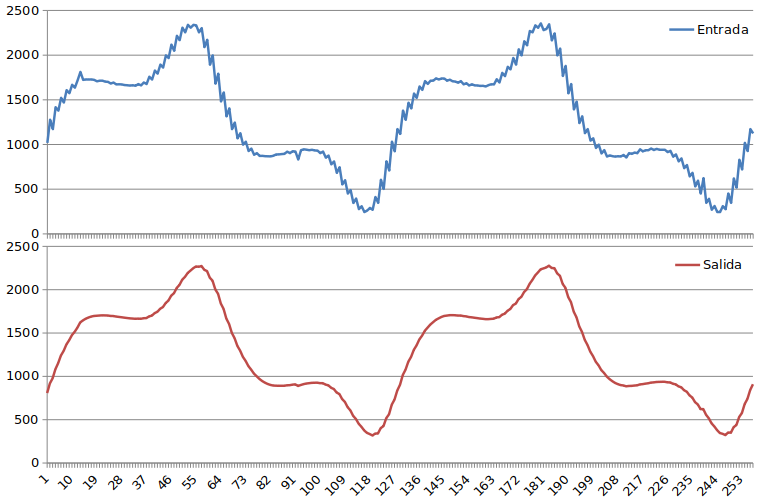
\includegraphics[scale=0.6]{./Figures/filtro.png}
	\caption{Filtro digital aplicado a la medición de corriente .}
	\label{fig:filtroPrue}
\end{figure}

\pagebreak

\section{Ensayos funcionales de integración}
Para los ensayos de integración, se decidió utilizar la metodología \textit{State transition testing} (STT) vista en la asignatura Testing de Software Embebido \citep{STT}. La metodología utilizada establece pasos sistemáticos para las pruebas de sistemas cuya funcionalidad depende de estados, de forma tal, de probar todos los caminos posibles y evitar dejar estados o condiciones sin cubrir. Para cada evento de entrada se debe verificar que:

\begin{enumerate}
	\item Se ejecutan las salidas correctas.
	\item El sistema cambia al estado correcto.
\end{enumerate}

Se tomó la decisión de utilizar esta metodología debido a que el equipo diseñado se comanda por el controlador principal, el cual, está construido sobre una máquina de estados finitos. Basado en lo anterior, tener una buena cobertura de dicha máquina de estados, asegura una buena cobertura del sistema general.

Para implementar la metodología propuesta, se tomaron las sub-máquinas de estados presentadas en la sección \ref{sec:ContSist}. Estas fueron definidas para las etapas de inicialización, de configuración, de caracterización y de reporte. El primer paso fue armar un árbol de transiciones para cada una de ellas, para luego, armar las tablas con los casos de pruebas. En el árbol de transiciones, las transacciones se marcan con un número en la línea de transición entre estados, este número es luego referenciado como ID en la primer columna de las tablas de casos de pruebas. La segunda columna corresponde a las entradas esperadas por parte de la persona encargada de la prueba. En caso de no requerir entrada, porque la transición de estado ocurre en forma automática, se coloca un guion '-' en dicha columna. 

Por otro lado, como salidas, se tiene el \textit{display}, lo enviado o recibido desde el servidor web, el sonido emitido por el \textit{buzzer} y la etiqueta impresa por la impresora. En cada paso, se verifica que dichas interfaces respondan como se espera.

A su vez que se probaron las secuencias definidas por los árboles de transiciones, se validó que dicho comportamiento es consistente con los requerimientos funcionales del sistema presentados en el capítulo \ref{Chapter2}. 

Para los ensayos que se presentan se miden las siguientes variables:
\begin{itemize}
 	\item Tensión en bobinado primario.
	\item Corriente que circula por el bobinado primario.
	\item Tensión en bobinado secundario.
	\item Corriente que circula por el bobinado secundario.
\end{itemize}

En la figura \ref{fig:EnsayoPrimario}, se muestra el banco de pruebas para el bobinado primario y en la figura \ref{fig:EnsayoSecu} se muestra el banco de pruebas para el bobinado secundario. Se puede notar que la medición de corriente carece de sentido cuando el bobinado en cuestión está abierto.

\begin{figure}[htpb]
	\centering
	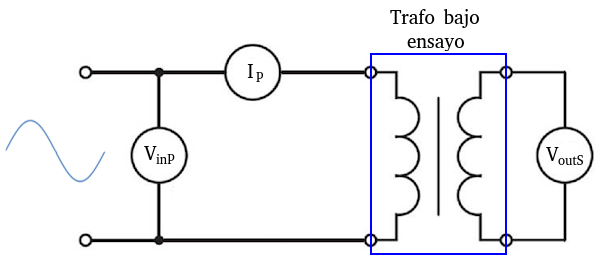
\includegraphics[scale=0.7]{./Figures/EnsayoPrimario.png}
	\caption{Valores medidos en el ensayo de bobinado primario.}
	\label{fig:EnsayoPrimario}
\end{figure}

\begin{figure}[htpb]
	\centering
	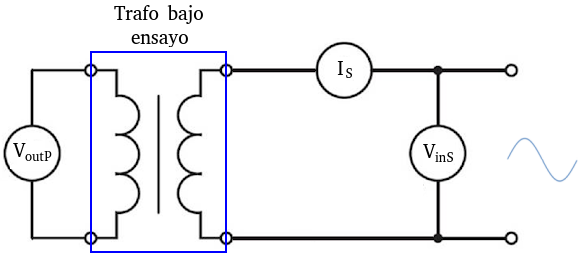
\includegraphics[scale=0.7]{./Figures/EnsayoSecu.png}
	\caption{Valores medidos en el ensayo de bobinado secundario.}
	\label{fig:EnsayoSecu}
\end{figure}

En la tabla \ref{tab:ref_med}, se muestran las convenciones de nombres utilizadas para referenciar los valores medidos de las figuras \ref{fig:EnsayoPrimario} y \ref{fig:EnsayoSecu} en las interfaces del sistema. En la primera columna de la tabla, se muestran los valores medidos y en las columnas subsiguientes, como estos son referenciados en el \textit{display}, en el servidor web y en la etiqueta impresa. 

\begin{table}[htpb]
\centering
\caption[Referencia valores medidos]{Referencia de valores medidos en el \textit{display}, el servidor web y la etiqueta impresa.}
\begin{tabular}{cccc}
\hline
\toprule
\textbf{Variable}                                       & \textbf{\textit{Display}} & \textbf{Servidor web}  & \textbf{Etiqueta} \\
\midrule
\begin{tabular}[c]{@{}c@{}}V$_{inP}$\\ {[}V{]}\end{tabular}  & -       & vinPrimary    & \begin{tabular}[c]{@{}c@{}}VL\\ Se muestra solo si el\\ transformador es rechazado\end{tabular} \\
\begin{tabular}[c]{@{}c@{}}I$_{P}$\\ {[}mA{]}\end{tabular}   & Ip      & iPrimary      & IP \\
\begin{tabular}[c]{@{}c@{}}V$_{outS}$\\ {[}V{]}\end{tabular} & Vs      & voutSecondary & VS \\
\begin{tabular}[c]{@{}c@{}}V$_{inS}$\\ {[}V{]}\end{tabular}  & -       & vinSecondary  & -  \\
\begin{tabular}[c]{@{}c@{}}V$_{outP}$\\ {[}V{]}\end{tabular} & -       & voutPrimary   & -  \\
\begin{tabular}[c]{@{}c@{}}I$_{S}$\\ {[}mA{]}\end{tabular}   & Is      & iSecondary    & IS \\
\bottomrule
\hline
\end{tabular}%
\label{tab:ref_med}
\end{table}

Se puede notar que no todos los valores medidos son mostrados en todas las interfaces. Esto último se debe a una restricción de espacio físico en el \textit{display} y la etiqueta.

\subsection{Pruebas de la etapa de inicialización}

Para la etapa de inicialización, se armó el árbol de transiciones mostrado en la figura \ref{fig:ArTrans_1}.

\begin{figure}[htpb]
	\centering
	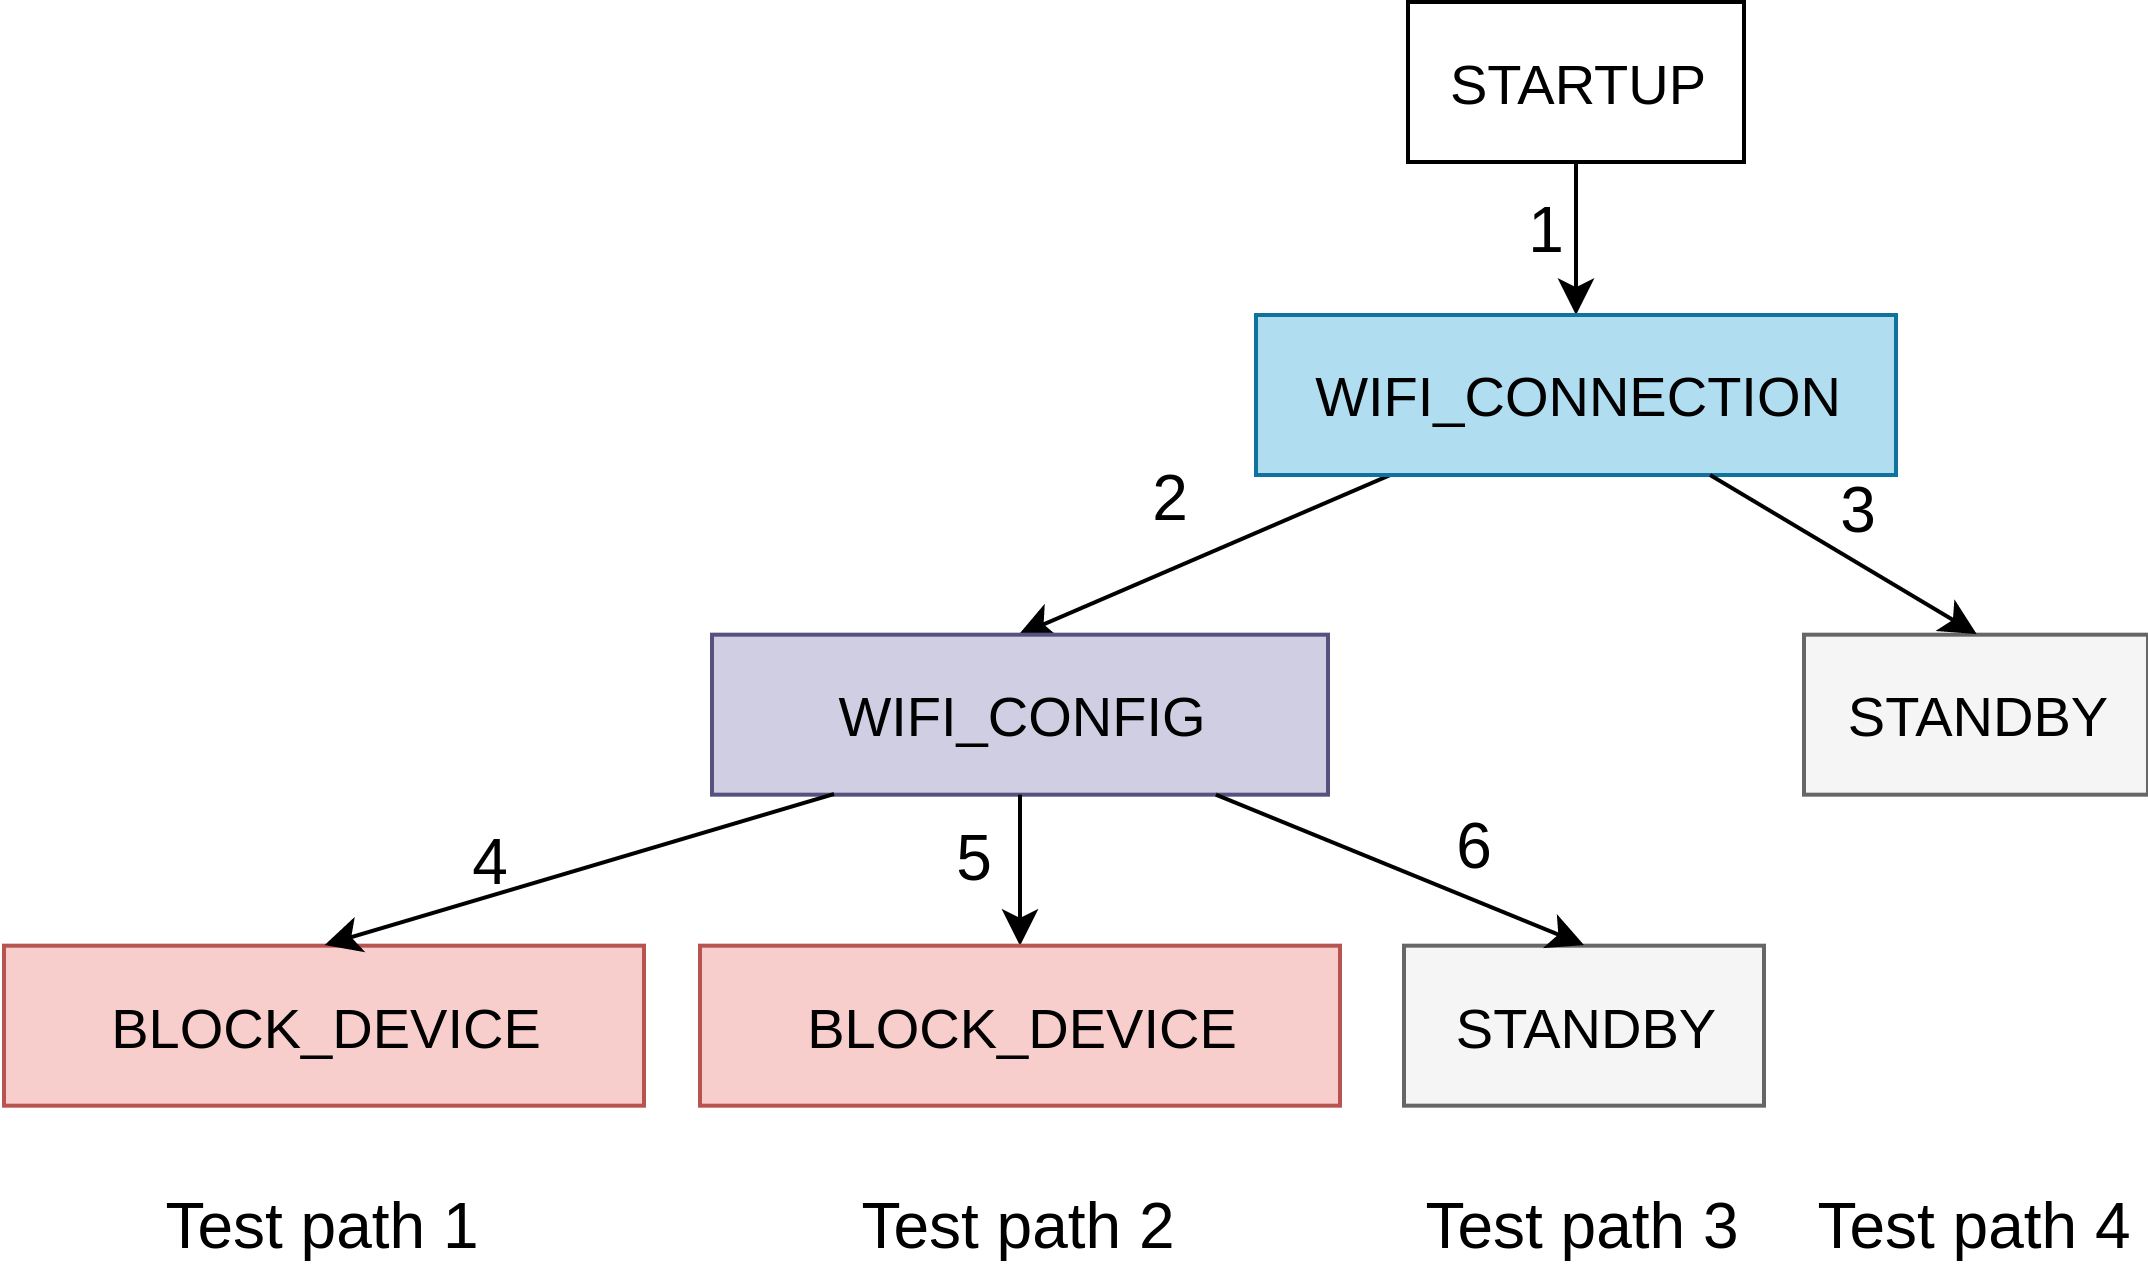
\includegraphics[scale=1]{./Figures/ArTrans_1.png}
	\caption{Árbol de transiciones: etapa de inicialización.}
	\label{fig:ArTrans_1}
\end{figure}

A partir del árbol generado, se obtuvieron cuatro caminos a verificar: \textit{test path} 1 a 4. De estos caminos, se armaron las tablas \ref{tab:pruIni_1} a \ref{tab:pruIni_4} con los casos de pruebas.

Para las pruebas de inicialización, se debe utilizar un equipo sin ningún dato de configuración cargado, de forma tal, de pasar por todos los pasos del árbol de transiciones.

Finalmente, en los casos en que el equipo queda bloqueado, \textit{test path} 1 y 2, se verificó que este no responde a ningún pulsador.

\subsubsection{Prueba del \textit{test path} 1}
\label{subsubsec:pruIni_1}

Condiciones iniciales: 

\begin{enumerate}
	\item Equipo desenergizado.
	\item Impresora encendida y conectada.
\end{enumerate}

En la tabla \ref{tab:pruIni_1}, se muestran los casos de pruebas para el \textit{test path} 1.

\begin{table}[htpb]
\centering
\caption[Prueba de la etapa de inicialización: \textit{test path} 1]{Casos de pruebas para el \textit{test path} 1.}
\resizebox{\textwidth}{!}{%
\begin{tabular}{cclc}
\hline
\toprule
\textbf{ID} & \textbf{Entrada}            & \textbf{Salida}  & \textbf{Estado}           \\
\midrule
-  & Encender el equipo & \begin{tabular}[c]{@{}l@{}}\textit{Display}: mensaje de bienvenida\\ \textit{Buzzer}: sin salida\\ Impresora: sin salida\end{tabular}                                                     & STARTUP          \\ \hline
1  & -                  & \begin{tabular}[c]{@{}l@{}}\textit{Display}: ``Estableciendo conexión WiFi''\\ \textit{Buzzer}: sin salida\\ Impresora: sin salida\end{tabular}                                             & WIFI\_CONNECTION \\ \hline
2  & -                  & \begin{tabular}[c]{@{}l@{}}\textit{Display}: ``Fallo al intentar conectar a WiFi''\\ "Desea configurar WiFi nuevamente?"\\ \textit{Buzzer}: sin salida\\ Impresora: sin salida\end{tabular} & WIFI\_CONFIG     \\ \hline
4  & Pulsar Cancelar    & \begin{tabular}[c]{@{}l@{}}\textit{Display}: ``Sin conexión WiFi Equipo bloqueado''\\ \textit{Buzzer}: sin salida\\ Impresora: sin salida\end{tabular}                                      & BLOCK\_DEVICE \\ 
\bottomrule
\hline
\end{tabular}%
}
\label{tab:pruIni_1}
\end{table}

\pagebreak
Resultado: el ensayo se superó con éxito. En la figura \ref{fig:pruIni_1_res}, se muestran las imágenes obtenidas del \textit{display} para cada paso.

\begin{figure}[!htpb]
     \centering
     \begin{subfigure}[b]{0.4\textwidth}
         \centering
         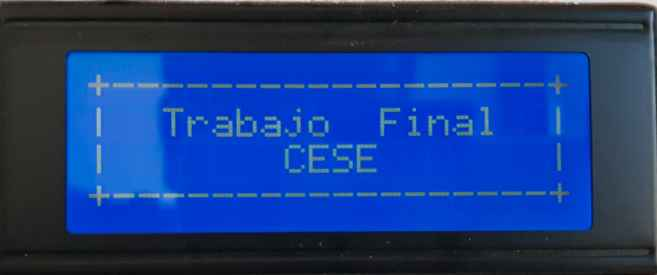
\includegraphics[width=1.1\textwidth]{./Figures/Bienvenida.jpeg}
         \caption{STARTUP.}
         \label{fig:pruIni_1_1}
     \end{subfigure}
     \hfill
     \begin{subfigure}[b]{0.4\textwidth}
         \centering
         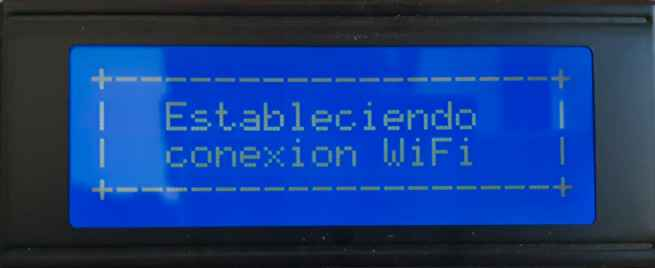
\includegraphics[width=1.1\textwidth]{./Figures/Esta_conex_WiFi.jpeg}
         \caption{WIFI\_CONNECTION}
         \label{fig:pruIni_1_2}
     \end{subfigure}
          \hfill
     \begin{subfigure}[b]{0.4\textwidth}
         \centering
         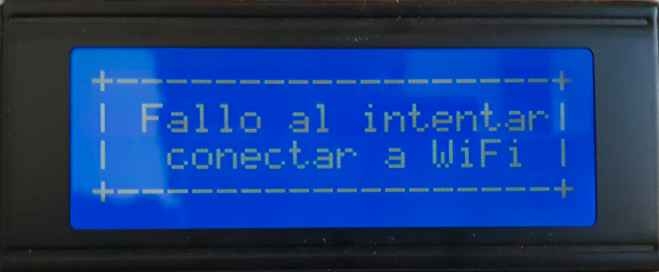
\includegraphics[width=1.1\textwidth]{./Figures/Fallo_con_WiFi.jpeg}
         \caption{WIFI\_CONFIG msg 1.}
         \label{fig:pruIni_1_3}
     \end{subfigure}
          \hfill
     \begin{subfigure}[b]{0.4\textwidth}
         \centering
         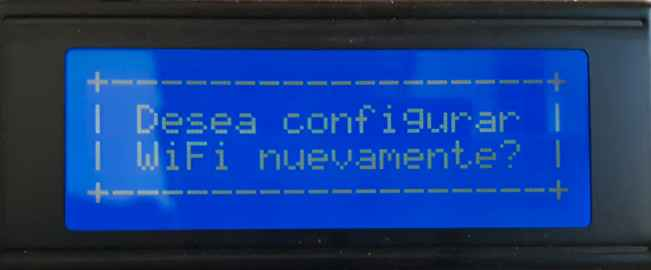
\includegraphics[width=1.1\textwidth]{./Figures/Conf_WiFi_nueva.jpeg}
         \caption{WIFI\_CONFIG msg 2.}
         \label{fig:pruIni_1_4}
     \end{subfigure}
          \hfill
     \begin{subfigure}[b]{0.4\textwidth}
         \centering
         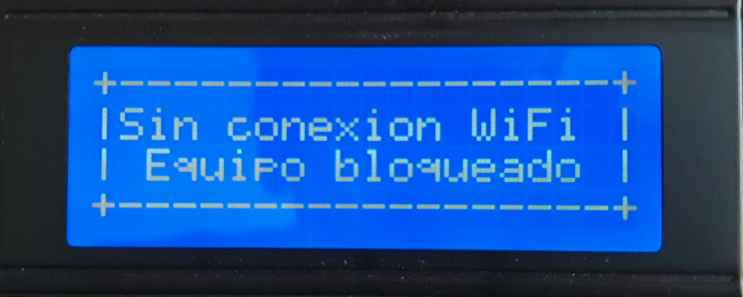
\includegraphics[width=1.1\textwidth]{./Figures/Sin_Conex_WiFi_Eq_Bloq.jpeg}
         \caption{BLOCK\_DEVICE.}
         \label{fig:pruIni_1_5}
     \end{subfigure}
        \caption{Resultado del \textit{test path} 1.}
        \label{fig:pruIni_1_res}
\end{figure}



\subsubsection{Prueba del \textit{test path} 2}
\label{subsubsec:pruIni_2}

Condiciones iniciales: 

\begin{enumerate}
	\item Equipo desenergizado.
	\item Impresora encendida y conectada.
	\item Teléfono móvil con la aplicación ESP-Touch instalada.
\end{enumerate}

En la tabla \ref{tab:pruIni_2}, se muestran los casos de pruebas para el \textit{test path} 2.

\begin{table}[htpb]
\centering
\caption[Prueba de la etapa de inicialización: \textit{test path} 2]{Casos de pruebas para el \textit{test path} 2.}
\resizebox{\textwidth}{!}{%
\begin{tabular}{cclc}
\hline
\toprule
\textbf{ID} & \textbf{Entrada}            & \textbf{Salida}  & \textbf{Estado}           \\
\midrule
-  & Encender el equipo & \begin{tabular}[c]{@{}l@{}}\textit{Display}: mensaje de bienvenida\\ \textit{Buzzer}: sin salida\\ Impresora: sin salida\end{tabular}                                                     & STARTUP          \\ \hline
1  & -                  & \begin{tabular}[c]{@{}l@{}}\textit{Display}: ``Estableciendo conexión WiFi''\\ \textit{Buzzer}: sin salida\\ Impresora: sin salida\end{tabular}                                             & WIFI\_CONNECTION \\ \hline
2  & -                  & \begin{tabular}[c]{@{}l@{}}\textit{Display}: ``Fallo al intentar conectar a WiFi''\\ "Desea configurar WiFi nuevamente?"\\ \textit{Buzzer}: sin salida\\ Impresora: sin salida\end{tabular} & WIFI\_CONFIG     \\ \hline
-  & Pulsar Configurar  & \begin{tabular}[c]{@{}l@{}}\textit{Display}: ``Configure WiFi por SmartConfig''\\ \textit{Buzzer}: sin salida\\ Impresora: sin salida\end{tabular}                                          & \begin{tabular}[c]{@{}c@{}}WIFI\_CONFIG\\ pseudoestado\end{tabular} \\ \hline
5  & \begin{tabular}[c]{@{}c@{}}Insertar datos \\ erróneos\\ en ESP-Touch\end{tabular} & \begin{tabular}[c]{@{}l@{}}\textit{Display}: ``Fallo al conectar por SmartConfig''\\ \textit{Buzzer}: sin salida\\ Impresora: sin salida\end{tabular}                                       & BLOCK\_DEVICE \\ 
\bottomrule
\hline
\end{tabular}%
}
\label{tab:pruIni_2}
\end{table}

Resultado: el ensayo se superó con éxito. En la figura \ref{fig:pruIni_2_res}, se muestran las imágenes obtenidas del \textit{display} para cada paso, se omiten las capturas de los primeros tres pasos ya que son iguales a las del \textit{test path} 1. 
 
\begin{figure}[!htpb]
     \centering
     \begin{subfigure}[b]{0.4\textwidth}
         \centering
         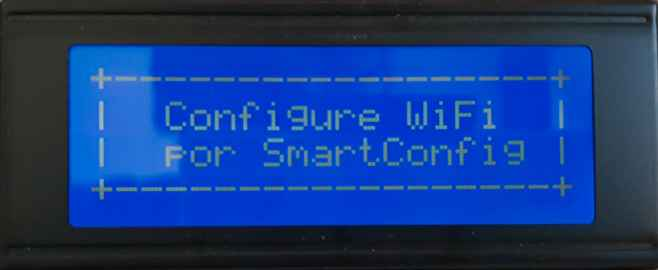
\includegraphics[width=1.1\textwidth]{./Figures/Conf_SmartConf.jpeg}
         \caption{WIFI\_CONFIG msg 4.}
         \label{fig:pruIni_2_1}
     \end{subfigure}
           \hfill
     \begin{subfigure}[b]{0.4\textwidth}
         \centering
         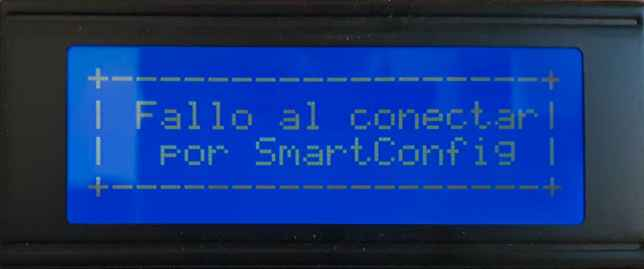
\includegraphics[width=1.1\textwidth]{./Figures/Fallo_SmartConf.jpeg}
         \caption{WIFI\_CONFIG msg 5.}
         \label{fig:pruIni_2_2}
     \end{subfigure}
           \hfill
     \begin{subfigure}[b]{0.4\textwidth}
         \centering
         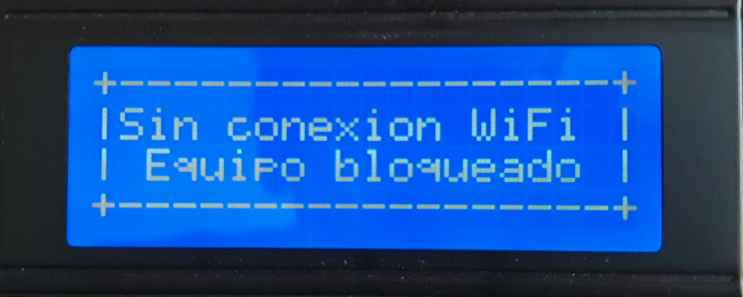
\includegraphics[width=1.1\textwidth]{./Figures/Sin_Conex_WiFi_Eq_Bloq.jpeg}
         \caption{BLOCK\_DEVICE.}
         \label{fig:pruIni_2_3}
     \end{subfigure}
        \caption{Resultado del \textit{test path} 2.}
        \label{fig:pruIni_2_res}
\end{figure}

En la figura \ref{fig:pruIni_2_ESPT}, se muestra una captura de pantalla de la aplicación ESP-Touch donde se observa la falla al intentar transferir las credenciales de Wi-Fi al equipo.

\begin{figure}[htpb]
	\centering
	\includegraphics[scale=0.4]{./Figures/ESP_Touch_fail.jpeg}
	\caption{Respuesta de la aplicación ESP-Touch.}
	\label{fig:pruIni_2_ESPT}
\end{figure}

\pagebreak
\subsubsection{Prueba del \textit{test path} 3}
\label{subsubsec:pruIni_3}

Condiciones iniciales: 

\begin{enumerate}
	\item Equipo desenergizado.
	\item Impresora encendida y conectada.
	\item Teléfono móvil con aplicación ESP-Touch instalada.
\end{enumerate}

En la tabla \ref{tab:pruIni_3}, se muestran los casos de pruebas para el \textit{test path} 3.

\begin{table}[htpb]
\centering
\caption[Prueba de la etapa de inicialización: \textit{test path} 3]{Casos de pruebas para el \textit{test path} 3.}
\resizebox{\textwidth}{!}{%
\begin{tabular}{cclc}
\hline
\toprule
\textbf{ID} & \textbf{Entrada}            & \textbf{Salida}  & \textbf{Estado}           \\
\midrule
-  & Encender el equipo & \begin{tabular}[c]{@{}l@{}}\textit{Display}: mensaje de bienvenida\\ \textit{Buzzer}: sin salida\\ Impresora: sin salida\end{tabular}                                                     & STARTUP          \\ \hline
1  & -                  & \begin{tabular}[c]{@{}l@{}}\textit{Display}: ``Estableciendo conexión WiFi''\\ \textit{Buzzer}: sin salida\\ Impresora: sin salida\end{tabular}                                             & WIFI\_CONNECTION \\ \hline
2  & -                  & \begin{tabular}[c]{@{}l@{}}\textit{Display}: ``Fallo al intentar conectar a WiFi''\\ "Desea configurar WiFi nuevamente?"\\ \textit{Buzzer}: sin salida\\ Impresora: sin salida\end{tabular} & WIFI\_CONFIG     \\ \hline
-  & Pulsar Configurar  & \begin{tabular}[c]{@{}l@{}}\textit{Display}: ``Configure WiFi por SmartConfig''\\ \textit{Buzzer}: sin salida\\ Impresora: sin salida\end{tabular}                                          & \begin{tabular}[c]{@{}c@{}}WIFI\_CONFIG\\ pseudoestado\end{tabular} \\ \hline
6  & \begin{tabular}[c]{@{}c@{}}Insertar los datos \\ correctos\\ en ESP-Touch\end{tabular} & \begin{tabular}[c]{@{}l@{}}\textit{Display}: ``Conectado a red WiFi''\\ \textit{Buzzer}: sin salida\\ Impresora: sin salida\end{tabular}  & STANDBY\\ 
\bottomrule
\hline
\end{tabular}%
}
\label{tab:pruIni_3}
\end{table}

\pagebreak
Resultado: el ensayo se superó con éxito. En la figura \ref{fig:pruIni_3_res}, se muestran las imágenes obtenidas del \textit{display} para cada paso, al igual que en la figura anterior, se omiten los primeros tres pasos. 

\begin{figure}[!htpb]
     \centering
     \begin{subfigure}[b]{0.4\textwidth}
         \centering
         \includegraphics[width=1.1\textwidth]{./Figures/Conf_SmartConf.jpeg}
         \caption{WIFI\_CONFIG msg 4.}
         \label{fig:pruIni_3_1}
     \end{subfigure}
           \hfill
     \begin{subfigure}[b]{0.4\textwidth}
         \centering
         \includegraphics[width=1.1\textwidth]{./Figures/Conect_to_WiFi.jpeg}
         \caption{WIFI\_CONFIG msg 5.}
         \label{fig:pruIni_3_2}
     \end{subfigure}
           \hfill
     \begin{subfigure}[b]{0.4\textwidth}
         \centering
         \includegraphics[width=1.1\textwidth]{./Figures/Esp_Conf.jpeg}
         \caption{STANDBY.}
         \label{fig:pruIni_3_3}
     \end{subfigure}
        \caption{Resultado del \textit{test path} 3.}
        \label{fig:pruIni_3_res}
\end{figure}

En la figura \ref{fig:pruIni_3_ESPT_1}, se muestra una captura de pantalla de la aplicación ESP-Touch donde se observa la conexión exitosa a la red Wi-Fi y la IP asignada al equipo en la red. Finalmente, en la figura \ref{fig:pruIni_3_ESPT_2} se muestra que, al conectarse el equipo a la red Wi-Fi, este responde al pedido de \textit{ping} desde el ordenador a la IP indicada por la aplicación ESP-Touch.

\pagebreak

\begin{figure}[htpb]
	\centering
	\includegraphics[scale=0.4]{./Figures/ESP_Touch_ok.jpeg}
	\caption{Respuesta de la aplicación ESP-Touch.}
	\label{fig:pruIni_3_ESPT_1}
\end{figure}

\begin{figure}[htpb]
	\centering
	\includegraphics[scale=0.8]{./Figures/ping.png}
	\caption{\textit{Ping} desde la consola a la IP devuelta por ESP-Touch.}
	\label{fig:pruIni_3_ESPT_2}
\end{figure}

\subsubsection{Prueba del \textit{test path} 4}
\label{subsubsec:pruIni_4}

Condiciones iniciales: 

\begin{enumerate}
	\item Equipo desenergizado.
	\item Impresora encendida y conectada.
\end{enumerate}


En la tabla \ref{tab:pruIni_4}, se muestran los casos de pruebas para el \textit{test path} 4.

\begin{table}[htpb]
\centering
\caption[Prueba de la etapa de inicialización: \textit{test path} 4]{Casos de pruebas para el \textit{test path} 4.}
\resizebox{\textwidth}{!}{%
\begin{tabular}{cclc}
\hline
\toprule
\textbf{ID} & \textbf{Entrada}            & \textbf{Salida}  & \textbf{Estado}           \\
\midrule
-  & Encender el equipo & \begin{tabular}[c]{@{}l@{}}\textit{Display}: mensaje de bienvenida\\ \textit{Buzzer}: sin salida\\ Impresora: sin salida\end{tabular}                                                     & STARTUP          \\ \hline
1  & -                  & \begin{tabular}[c]{@{}l@{}}\textit{Display}: ``Estableciendo conexión WiFi''\\ \textit{Buzzer}: sin salida\\ Impresora: sin salida\end{tabular}                                             & WIFI\_CONNECTION \\ \hline
3  & - & \begin{tabular}[c]{@{}l@{}}\textit{Display}: ``Esperando... Configuración''\\ \textit{Buzzer}: sin salida\\ Impresora: sin salida\end{tabular}  & STANDBY\\ 
\bottomrule
\hline
\end{tabular}%
}
\label{tab:pruIni_4}
\end{table}

\pagebreak

Resultado: el ensayo se superó con éxito. En la figura \ref{fig:pruIni_4_res}, se muestran las imágenes obtenidas del \textit{display} para cada paso. En este caso, el equipo no requiere interacción con el operador ya que, las credenciales de Wi-Fi fueron correctamente configuradas en el paso anterior y se guardaron en la memoria no volátil del equipo.

\begin{figure}[!htpb]
     \centering
     \begin{subfigure}[b]{0.4\textwidth}
         \centering
         \includegraphics[width=1.1\textwidth]{./Figures/Bienvenida.jpeg}
         \caption{STARTUP.}
         \label{fig:pruIni_4_1}
     \end{subfigure}
           \hfill
     \begin{subfigure}[b]{0.4\textwidth}
         \centering
         \includegraphics[width=1.1\textwidth]{./Figures/Esta_conex_WiFi.jpeg}
         \caption{WIFI\_CONNECTION}
         \label{fig:pruIni_4_2}
     \end{subfigure}
           \hfill
     \begin{subfigure}[b]{0.4\textwidth}
         \centering
         \includegraphics[width=1.1\textwidth]{./Figures/Esp_Conf.jpeg}
         \caption{STANDBY.}
         \label{fig:pruIni_4_3}
     \end{subfigure}
        \caption{Resultado del \textit{test path} 4.}
        \label{fig:pruIni_4_res}
\end{figure}

\subsection{Pruebas de la etapa de configuración}

Para la etapa de configuración, se armó el árbol de transiciones mostrado en la figura \ref{fig:ArTrans_2}. A partir de este, se obtuvieron tres caminos a verificar: \textit{test path} 5 a 7, de los cuales, surgen las tablas \ref{tab:pruConf_5} a \ref{tab:pruConf_7} con los casos de pruebas.

\begin{figure}[htpb]
	\centering
	\includegraphics[scale=1]{./Figures/ArTrans_2.png}
	\caption{Árbol de transiciones: etapa de configuración.}
	\label{fig:ArTrans_2}
\end{figure}

Para las pruebas de configuración, se parte siempre del estado STANDBY, por lo tanto, se tiene que superar el \textit{test path} 4 del estado de inicialización para poder comenzar las pruebas de esta etapa.

\pagebreak

A partir de estos ensayos, se pudieron validar los requerimientos: 
\begin{itemize}
\item Requerimientos 1 y 2 de la sección \ref{subsec:ReqFun}.
\item Requerimientos 1 y 2 de la sección \ref{subsec:ReqCom}.
\item Requerimientos 1.a y 2.a de la sección \ref{subsec:ReqUsu}.
\end{itemize}

\subsubsection{Prueba del \textit{test path} 5}
\label{subsubsec:pruConf_5}

Condiciones iniciales: 

\begin{enumerate}
	\item Equipo energizado y \textit{test path} 4 corrido.
	\item Impresora encendida y conectada.
\end{enumerate}

En la tabla \ref{tab:pruConf_5}, se muestran los casos de pruebas para el \textit{test path} 5.

\begin{table}[htpb]
\centering
\caption[Prueba de la etapa de configuración: \textit{test path} 5]{Casos de pruebas para el \textit{test path} 5.}
\resizebox{\textwidth}{!}{%
\begin{tabular}{cclc}
\hline
\toprule
\textbf{ID} & \textbf{Entrada}            & \textbf{Salida}  & \textbf{Estado}           \\
\midrule
-  & -        & \begin{tabular}[c]{@{}l@{}}\textit{Display}: ``Esperando... Configuración''\\ \textit{Buzzer}: sin salida\\ Impresora: sin salida\end{tabular} & STANDBY           \\ \hline
7  & Pulsar Testear & \begin{tabular}[c]{@{}l@{}}\textit{Display}: ``Equipo no configurado''\\ \textit{Buzzer}: sin salida\\ Impresora: sin salida\end{tabular}      & NOT\_CONFIGURATED \\ \hline
9  & -        & \begin{tabular}[c]{@{}l@{}}\textit{Display}: ``Esperando... Configuración''\\ \textit{Buzzer}: sin salida\\ Impresora: sin salida\end{tabular} & STANDBY          
\\ 
\bottomrule
\hline
\end{tabular}%
}
\label{tab:pruConf_5}
\end{table}

Resultado: el ensayo se superó con éxito. En la figura \ref{fig:pruConf_5_res}, se muestran las imágenes obtenidas del \textit{display} para cada paso.

\begin{figure}[!htpb]
     \centering
     \begin{subfigure}[b]{0.4\textwidth}
         \centering
         \includegraphics[width=1.1\textwidth]{./Figures/Esp_Conf.jpeg}
         \caption{STANDBY.}
         \label{fig:pruConf_5_1}
     \end{subfigure}
           \hfill
     \begin{subfigure}[b]{0.4\textwidth}
         \centering
         \includegraphics[width=1.1\textwidth]{./Figures/Eq_no_conf.jpeg}
         \caption{NOT\_CONFIGURATED.}
         \label{fig:pruConf_5_2}
     \end{subfigure}
           \hfill
     \begin{subfigure}[b]{0.4\textwidth}
         \centering
         \includegraphics[width=1.1\textwidth]{./Figures/Esp_Conf.jpeg}
         \caption{STANDBY.}
         \label{fig:pruConf_5_3}
     \end{subfigure}
        \caption{Resultado del \textit{test path} 5.}
        \label{fig:pruConf_5_res}
\end{figure}

\pagebreak

\subsubsection{Prueba del \textit{test path} 6}
\label{subsubsec:pruConf_6}

Condiciones iniciales: 

\begin{enumerate}
	\item Equipo energizado y \textit{test path} 4 corrido.
	\item Impresora encendida y conectada.
	\item Servidor web no disponible. Se le pidió al cliente que detenga el servidor web para llevar a cabo la prueba.
\end{enumerate}

En la tabla \ref{tab:pruConf_6}, se muestran los casos de pruebas para el \textit{test path} 6.

\begin{table}[htpb]
\centering
\caption[Prueba de la etapa de configuración: \textit{test path} 6]{Casos de pruebas para el \textit{test path} 6.}
\resizebox{\textwidth}{!}{%
\begin{tabular}{cclc}
\hline
\toprule
\textbf{ID} & \textbf{Entrada}            & \textbf{Salida}  & \textbf{Estado}           \\
\midrule
-  & -        & \begin{tabular}[c]{@{}l@{}}\textit{Display}: ``Esperando... Configuración''\\ \textit{Buzzer}: sin salida\\ Impresora: sin salida\end{tabular} & STANDBY           \\ \hline
8  & Pulsar Configurar                                                              & \begin{tabular}[c]{@{}l@{}}\textit{Display}: ``Configurando Espere...''\\ \textit{Buzzer}: sin salida\\ Impresora: sin salida\end{tabular}     & CONFIGURATING       \\ \hline
10 & \begin{tabular}[c]{@{}c@{}}Servidor web\\no disponible\end{tabular} & \begin{tabular}[c]{@{}l@{}}\textit{Display}: ``Falla en configuración''\\ \textit{Buzzer}: sin salida\\ Impresora: sin salida\end{tabular}     & CONFIGURATION\_FAIL \\ \hline
12  & -        & \begin{tabular}[c]{@{}l@{}}\textit{Display}: ``Esperando... Configuración''\\ \textit{Buzzer}: sin salida\\ Impresora: sin salida\end{tabular} & STANDBY          
\\ 
\bottomrule
\hline
\end{tabular}%
}
\label{tab:pruConf_6}
\end{table}

Resultado: el ensayo se superó con éxito. En la figura \ref{fig:pruConf_6_res}, se muestran las imágenes obtenidas del \textit{display} para cada paso.

\begin{figure}[!htpb]
     \centering
     \begin{subfigure}[b]{0.4\textwidth}
         \centering
         \includegraphics[width=1.1\textwidth]{./Figures/Esp_Conf.jpeg}
         \caption{STANDBY.}
         \label{fig:pruConf_6_1}
     \end{subfigure}
           \hfill
     \begin{subfigure}[b]{0.4\textwidth}
         \centering
         \includegraphics[width=1.1\textwidth]{./Figures/Conf_esp.jpeg}
         \caption{CONFIGURATING.}
         \label{fig:pruConf_6_2}
     \end{subfigure}
           \hfill
     \begin{subfigure}[b]{0.4\textwidth}
         \centering
         \includegraphics[width=1.1\textwidth]{./Figures/Falla_conf.jpeg}
         \caption{CONFIGURATION\_FAIL.}
         \label{fig:pruConf_6_3}
     \end{subfigure}
           \hfill
     \begin{subfigure}[b]{0.4\textwidth}
         \centering
         \includegraphics[width=1.1\textwidth]{./Figures/Esp_Conf.jpeg}
         \caption{STANDBY.}
         \label{fig:pruConf_6_4}
     \end{subfigure}
        \caption{Resultado del \textit{test path} 6.}
        \label{fig:pruConf_6_res}
\end{figure}

\pagebreak

\subsubsection{Prueba del \textit{test path} 7}
\label{subsubsec:pruConf_7}

Condiciones iniciales: 

\begin{enumerate}
	\item Equipo energizado y \textit{test path} 4 corrido.
	\item Impresora encendida y conectada.
	\item Servidor web en condiciones operativas y con datos validos. Los datos cargados en el servidor se muestran en la figura \ref{fig:serv_web_conf}. Para obtener esta información se envío un comando GET de HTTP al servidor web a través del explorador Firefox. Los datos se encuentran en formato JSON.
\end{enumerate}

\begin{figure}[htpb]
	\centering
	\includegraphics[scale=1]{./Figures/serv_web_falla_conf.png}
	\caption{Datos de configuración en el servidor web.}
	\label{fig:serv_web_conf}
\end{figure}

En la tabla \ref{tab:pruConf_7}, se muestran los casos de pruebas para el \textit{test path} 7.

\begin{table}[htpb]
\centering
\caption[Prueba de la etapa de configuración: \textit{test path} 7]{Casos de pruebas para el \textit{test path} 7.}
\resizebox{\textwidth}{!}{%
\begin{tabular}{cclc}
\hline
\toprule
\textbf{ID} & \textbf{Entrada}            & \textbf{Salida}  & \textbf{Estado}           \\
\midrule
-  & -        & \begin{tabular}[c]{@{}l@{}}\textit{Display}: ``Esperando... Configuración''\\ \textit{Buzzer}: sin salida\\ Impresora: sin salida\end{tabular} & STANDBY           \\ \hline
8  & Pulsar Configurar                                                              & \begin{tabular}[c]{@{}l@{}}\textit{Display}: ``Configurando Espere...''\\ \textit{Buzzer}: sin salida\\ Impresora: sin salida\end{tabular}     & CONFIGURATING       \\ \hline
11 & \begin{tabular}[c]{@{}c@{}}Servidor web\\ con datos \\ válidos\end{tabular} & \begin{tabular}[c]{@{}l@{}}\textit{Display}: mostrar los datos del servidor web\\ \textit{Buzzer}: sin salida\\ Impresora: sin salida\end{tabular}     & CONFIGURATION\_OK \\ \hline
13  & -        & \begin{tabular}[c]{@{}l@{}}\textit{Display}: mostrar los datos del servidor web\\ \textit{Buzzer}: sin salida\\ Impresora: sin salida\end{tabular} & STANDBY          
\\ 
\bottomrule
\hline
\end{tabular}%
}
\label{tab:pruConf_7}
\end{table}

Resultado: el ensayo se superó con éxito. En la figura \ref{fig:pruConf_7_res}, se muestran las imágenes obtenidas del \textit{display} para cada paso. 

\begin{figure}[!htpb]
     \centering
     \begin{subfigure}[b]{0.4\textwidth}
         \centering
         \includegraphics[width=1.1\textwidth]{./Figures/Esp_Conf.jpeg}
         \caption{STANDBY.}
         \label{fig:pruConf_7_1}
     \end{subfigure}
           \hfill
     \begin{subfigure}[b]{0.4\textwidth}
         \centering
         \includegraphics[width=1.1\textwidth]{./Figures/Conf_esp.jpeg}
         \caption{CONFIGURATING.}
         \label{fig:pruConf_7_2}
     \end{subfigure}
           \hfill
     \begin{subfigure}[b]{0.4\textwidth}
         \centering
         \includegraphics[width=1.1\textwidth]{./Figures/pru_fail.jpeg}
         \caption{CONFIGURATION\_OK.}
         \label{fig:pruConf_7_3}
     \end{subfigure}
           \hfill
     \begin{subfigure}[b]{0.4\textwidth}
         \centering
         \includegraphics[width=1.1\textwidth]{./Figures/pru_fail.jpeg}
         \caption{STANDBY.}
         \label{fig:pruConf_7_4}
     \end{subfigure}
        \caption{Resultado del \textit{test path} 7.}
        \label{fig:pruConf_7_res}
\end{figure}

En las subfiguras \ref{fig:pruConf_7_3} y \ref{fig:pruConf_7_4}, correspondientes a los pasos 11 y 13, se muestran, en el \textit{display}, algunos de los datos obtenidos del servidor web. Se verificó que los datos de las subfiguras coincidan con los datos almacenados en el servidor web que se presentaron en la figura \ref{fig:serv_web_conf}. Para realizar esta comparación se debe tener en cuenta las referencias mostradas en la tabla \ref{tab:ref_med}.

\subsection{Pruebas de la etapa de caracterización}

Para la etapa de caracterización, se armó el árbol de transiciones mostrado en la figura \ref{fig:ArTrans_3}. A partir de este, se obtuvieron cuatro caminos a verificar: \textit{test path} 8 a 11, de los cuales, surgen las tablas \ref{tab:pruCarac_8} a \ref{tab:pruCarac_11} con los casos de pruebas.

\begin{figure}[htpb]
	\centering
	\includegraphics[scale=0.95]{./Figures/ArTrans_3.png}
	\caption{Árbol de transiciones: etapa de caracterización.}
	\label{fig:ArTrans_3}
\end{figure}

Para las pruebas de caracterización, se parte desde el estado STANDBY con el equipo configurado, por lo tanto, se tiene que superar el \textit{test path} 7 del estado de configuración para poder comenzar las pruebas de esta etapa.

A partir de estos ensayos, se pudieron validar los requerimientos: 
\begin{itemize}
\item Requerimientos 3 y 4 de la sección \ref{subsec:ReqFun}.
\item Requerimiento 3 de la sección \ref{subsec:ReqCom}.
\item Requerimientos 1.b, 1.c, 2.a, 2.b, 2.c, 2.d y 3 de la sección \ref{subsec:ReqUsu}.
\end{itemize}


\subsubsection{Prueba del \textit{test path} 8}
\label{subsubsec:pruCarac_8}

Condiciones iniciales: 

\begin{enumerate}
	\item Equipo energizado y \textit{test path} 7 corrido.
	\item Impresora encendida y conectada.
	\item Tapa de seguridad abierta.
\end{enumerate}

En la tabla \ref{tab:pruCarac_8}, se muestran los casos de pruebas para el \textit{test path} 8.

\begin{table}[htpb]
\centering
\caption[Prueba de la etapa de caracterización: \textit{test path} 8]{Casos de pruebas para el \textit{test path} 8.}
\resizebox{\textwidth}{!}{%
\begin{tabular}{cclc}
\hline
\toprule
\textbf{ID} & \textbf{Entrada}            & \textbf{Salida}  & \textbf{Estado}           \\
\midrule
-  & \begin{tabular}[c]{@{}c@{}}Tapa de seguridad\\ abierta \end{tabular}       & \begin{tabular}[c]{@{}l@{}}\textit{Display}: mostrar los datos del servidor web\\ \textit{Buzzer}: sin salida\\ Impresora: sin salida\end{tabular} & STANDBY           \\ \hline
14  & Pulsar Testear & \begin{tabular}[c]{@{}l@{}}\textit{Display}: ``Tapa de seguridad abierta''\\ \textit{Buzzer}: sin salida\\ Impresora: sin salida\end{tabular}      & SAFETY\_SWITCH\_OPEN \\ \hline
16  & -        & \begin{tabular}[c]{@{}l@{}}\textit{Display}: mostrar los datos del servidor web\\ \textit{Buzzer}: sin salida\\ Impresora: sin salida\end{tabular} & STANDBY          
\\ 
\bottomrule
\hline
\end{tabular}%
}
\label{tab:pruCarac_8}
\end{table}

Resultado: el ensayo se superó con éxito. En la figura \ref{fig:pruConf_8_res}, se muestran las imágenes obtenidas del \textit{display} para cada paso. 

\begin{figure}[!htpb]
     \centering
     \begin{subfigure}[b]{0.4\textwidth}
         \centering
         \includegraphics[width=1.1\textwidth]{./Figures/pru_fail.jpeg}
         \caption{STANDBY.}
         \label{fig:pruConf_8_1}
     \end{subfigure}
           \hfill
     \begin{subfigure}[b]{0.4\textwidth}
         \centering
         \includegraphics[width=1.1\textwidth]{./Figures/tapa_abierta.jpeg}
         \caption{SAFETY\_SWITCH\_OPEN.}
         \label{fig:pruConf_8_2}
     \end{subfigure}
           \hfill
     \begin{subfigure}[b]{0.4\textwidth}
         \centering
         \includegraphics[width=1.1\textwidth]{./Figures/pru_fail.jpeg}
         \caption{STANDBY.}
         \label{fig:pruConf_8_3}
     \end{subfigure}
        \caption{Resultado del \textit{test path} 8.}
        \label{fig:pruConf_8_res}
\end{figure}

\subsubsection{Prueba del \textit{test path} 9}
\label{subsubsec:pruCarac_9}

Condiciones iniciales: 

\begin{enumerate}
	\item Equipo energizado y \textit{test path} 7 corrido.
	\item Impresora encendida y conectada.
	\item Tapa de seguridad cerrada.
\end{enumerate}

En la tabla \ref{tab:pruCarac_9}, se muestran los casos de pruebas para el \textit{test path} 9.

\begin{table}[htpb]
\centering
\caption[Prueba de la etapa de caracterización: \textit{test path} 9]{Casos de pruebas para el \textit{test path} 9.}
\resizebox{\textwidth}{!}{%
\begin{tabular}{cclc}
\hline
\toprule
\textbf{ID} & \textbf{Entrada}            & \textbf{Salida}  & \textbf{Estado}           \\
\midrule
-  & \begin{tabular}[c]{@{}c@{}}Tapa de seguridad\\ cerrada\end{tabular}      & \begin{tabular}[c]{@{}l@{}}\textit{Display}: mostrar los datos del servidor web\\ \textit{Buzzer}: sin salida\\ Impresora: sin salida\end{tabular} & STANDBY           \\ \hline
15 & Pulsar Testear                                                      & \begin{tabular}[c]{@{}l@{}}\textit{Display}: mostrar los datos del servidor web\\ \textit{Buzzer}: sin salida\\ Impresora: sin salida\end{tabular} & MEASURE\_PRIMARY \\ \hline
17 & Pulsar Cancelar                                                     & \begin{tabular}[c]{@{}l@{}}\textit{Display}: ``Cancelando espere...''\\ \textit{Buzzer}: sin salida\\ Impresora: sin salida\end{tabular}         & CANCEL           \\ \hline
19  & -        & \begin{tabular}[c]{@{}l@{}}\textit{Display}: mostrar los datos del servidor web\\ \textit{Buzzer}: sin salida\\ Impresora: sin salida\end{tabular} & STANDBY          
\\ 
\bottomrule
\hline
\end{tabular}%
}
\label{tab:pruCarac_9}
\end{table}

Resultado: el ensayo se superó con éxito. En la figura \ref{fig:pruConf_9_res}, se muestran las imágenes obtenidas del \textit{display} para cada paso. A partir de la misma secuencia de prueba, se probó la apertura de la tapa de seguridad una vez iniciado el ensayo, es decir, en vez de pulsar Cancelar en el paso 17, se procedió a abrir la tapa de seguridad y el resultado obtenido fue equivalente.

\begin{figure}[!htpb]
     \centering
     \begin{subfigure}[b]{0.4\textwidth}
         \centering
         \includegraphics[width=1.1\textwidth]{./Figures/pru_fail.jpeg}
         \caption{STANDBY.}
         \label{fig:pruConf_9_1}
     \end{subfigure}
          \hfill
     \begin{subfigure}[b]{0.4\textwidth}
         \centering
         \includegraphics[width=1.1\textwidth]{./Figures/pru_fail.jpeg}
         \caption{MEASURE\_PRIMARY.}
         \label{fig:pruConf_9_2}
     \end{subfigure}
           \hfill
     \begin{subfigure}[b]{0.4\textwidth}
         \centering
         \includegraphics[width=1.1\textwidth]{./Figures/cancel.jpeg}
         \caption{CANCEL.}
         \label{fig:pruConf_9_3}
     \end{subfigure}
           \hfill
     \begin{subfigure}[b]{0.4\textwidth}
         \centering
         \includegraphics[width=1.1\textwidth]{./Figures/pru_fail.jpeg}
         \caption{STANDBY.}
         \label{fig:pruConf_9_4}
     \end{subfigure}
        \caption{Resultado del \textit{test path} 9.}
        \label{fig:pruConf_9_res}
\end{figure}

\subsubsection{Prueba del \textit{test path} 10}
\label{subsubsec:pruCarac_10}

Condiciones iniciales: 

\begin{enumerate}
	\item Equipo energizado y \textit{test path} 7 corrido.
	\item Impresora encendida y conectada.
	\item Tapa de seguridad cerrada.
\end{enumerate}

En la tabla \ref{tab:pruCarac_10}, se muestran los casos de pruebas para el \textit{test path} 10.

\begin{table}[htpb]
\centering
\caption[Prueba de la etapa de caracterización: \textit{test path} 10]{Casos de pruebas para el \textit{test path} 10.}
\resizebox{\textwidth}{!}{%
\begin{tabular}{cclc}
\hline
\toprule
\textbf{ID} & \textbf{Entrada}            & \textbf{Salida}  & \textbf{Estado}           \\
\midrule
-  & \begin{tabular}[c]{@{}c@{}}Tapa de seguridad\\ cerrada\end{tabular}      & \begin{tabular}[c]{@{}l@{}}\textit{Display}: mostrar los datos del servidor web\\ \textit{Buzzer}: sin salida\\ Impresora: sin salida\end{tabular} & STANDBY           \\ \hline
15 & Pulsar Testear                                                      & \begin{tabular}[c]{@{}l@{}}\textit{Display}: mostrar los datos del servidor web\\ \textit{Buzzer}: sin salida\\ Impresora: sin salida\end{tabular} & MEASURE\_PRIMARY \\ \hline
18 & -                                                      & \begin{tabular}[c]{@{}l@{}}\textit{Display}: mostrar los datos del servidor web\\ \textit{Buzzer}: sin salida\\ Impresora: sin salida\end{tabular} & MEASURE\_SECONDARY \\ \hline
20 & Pulsar Cancelar                                                     & \begin{tabular}[c]{@{}l@{}}\textit{Display}: ``Cancelando espere...''\\ \textit{Buzzer}: sin salida\\ Impresora: sin salida\end{tabular}         & CANCEL           \\ \hline
22  & -        & \begin{tabular}[c]{@{}l@{}}\textit{Display}: mostrar los datos del servidor web\\ \textit{Buzzer}: sin salida\\ Impresora: sin salida\end{tabular} & STANDBY          
\\ 
\bottomrule
\hline
\end{tabular}%
}
\label{tab:pruCarac_10}
\end{table}

Resultado: el ensayo se superó con éxito. Dado que los resultados son los mismos que en el ensayo anterior, se decidió omitir las figuras. Por otro lado, se probó la apertura de la tapa de seguridad siguiendo el mismo procedimiento que en el caso anterior.

\pagebreak

\subsubsection{Prueba del \textit{test path} 11}
\label{subsubsec:pruCarac_11}

Condiciones iniciales: 

\begin{enumerate}
	\item Equipo energizado y \textit{test path} 7 corrido.
	\item Impresora encendida y conectada.
	\item Servidor web en condiciones operativas.
	\item Tapa de seguridad cerrada.
\end{enumerate}

En la tabla \ref{tab:pruCarac_11}, se muestran los casos de pruebas para el \textit{test path} 11.

\begin{table}[htpb]
\centering
\caption[Prueba de la etapa de caracterización: \textit{test path} 11]{Casos de pruebas para el \textit{test path} 11.}
\resizebox{\textwidth}{!}{%
\begin{tabular}{cclc}
\hline
\toprule
\textbf{ID} & \textbf{Entrada}            & \textbf{Salida}  & \textbf{Estado}           \\
\midrule
-  & \begin{tabular}[c]{@{}c@{}}Tapa de seguridad\\ cerrada\end{tabular}      & \begin{tabular}[c]{@{}l@{}}\textit{Display}: mostrar los datos del servidor web\\ \textit{Buzzer}: sin salida\\ Impresora: sin salida\end{tabular} & STANDBY           \\ \hline
15 & Pulsar Testear                                                      & \begin{tabular}[c]{@{}l@{}}\textit{Display}: mostrar los datos del servidor web\\ \textit{Buzzer}: sin salida\\ Impresora: sin salida\end{tabular} & MEASURE\_PRIMARY \\ \hline
18 & -                                                      & \begin{tabular}[c]{@{}l@{}}\textit{Display}: mostrar los datos del servidor web\\ \textit{Buzzer}: sin salida\\ Impresora: sin salida\end{tabular} & MEASURE\_SECONDARY \\ \hline
21 & -                                                     & \begin{tabular}[c]{@{}l@{}}\textit{Display}: mostrar los resultados del ensayo\\ \textit{Buzzer}: emitir sonido acorde al \\ resultado del ensayo\\ Impresora: imprimir etiqueta acorde al \\ resultado del ensayo\end{tabular}         & REPORT           \\ \hline
23  & -        & \begin{tabular}[c]{@{}l@{}}\textit{Display}: mostrar los datos del servidor web\\ \textit{Buzzer}: sin salida\\ Impresora: sin salida\end{tabular} & STANDBY          
\\ 
\bottomrule
\hline
\end{tabular}%
}
\label{tab:pruCarac_11}
\end{table}

Dado que este ensayo es el encargado de probar que las mediciones y que las comparaciones se realicen apropiadamente, este se corrió varias veces con diferentes transformadores y diferentes datos en el servidor web. Con las variantes anteriores, se pudo verificar y validar que el equipo genere los resultados esperados para transformadores aprobados o rechazados.

En el primer caso, se realiza una prueba para un transformador rechazado. En la tabla \ref{tab:pruCarac_11_res}, se muestran los resultados esperados para este ensayo. En las columnas de máximo y mínimo se muestran los valores configurados desde el servidor web, los cuales, coinciden con los mostrados en la figura \ref{fig:serv_web_conf} del \textit{test path} 7.

\begin{table}[htpb]
\centering
\caption[Ensayo para transformador rechazado]{Resultados esperados para el \textit{test path} 11 en la condición de transformador rechazado}
\resizebox{0.6\textwidth}{!}{%
\begin{tabular}{ccccc}
\hline
\toprule
\textbf{Variable} & \textbf{Máximo} & \textbf{Mínimo} & \begin{tabular}[c]{@{}c@{}}\textbf{Valor}\\ \textbf{medido}\end{tabular} & \begin{tabular}[c]{@{}c@{}}\textbf{Resultado}\\ \textbf{esperado}\end{tabular} \\
\midrule
\begin{tabular}[c]{@{}c@{}}V$_{outS}$\\ {[}V{]}\end{tabular} & 17     & 14     & 17.7  & FALLA   \\
\begin{tabular}[c]{@{}c@{}}I$_{P}$\\ {[}mA{]}\end{tabular}   & 70     & 15     & 100   & FALLA   \\
\begin{tabular}[c]{@{}c@{}}I$_{S}$\\ {[}mA{]}\end{tabular}   & 400    & 100    & 977   & FALLA   \\                                                    
\bottomrule
\hline
\end{tabular}%
}
\label{tab:pruCarac_11_res}
\end{table}

Resultados para un transformador rechazado: el ensayo se superó con éxito. En la figura \ref{fig:pruConf_11_res_a}, se muestran las imágenes obtenidas del \textit{display} para cada paso.

\begin{figure}[!htpb]
     \centering
     \begin{subfigure}[b]{0.4\textwidth}
         \centering
         \includegraphics[width=1.1\textwidth]{./Figures/pru_fail.jpeg}
         \caption{MEASURE\_SECONDARY.}
         \label{fig:pruConf_11_1_a}
     \end{subfigure}
          \hfill
     \begin{subfigure}[b]{0.4\textwidth}
         \centering
         \includegraphics[width=1.1\textwidth]{./Figures/rechazado.jpeg}
         \caption{REPORT.}
         \label{fig:pruConf_11_2_a}
     \end{subfigure}
           \hfill
     \begin{subfigure}[b]{0.4\textwidth}
         \centering
         \includegraphics[width=1.1\textwidth]{./Figures/pru_fail.jpeg}
         \caption{STANDBY.}
         \label{fig:pruConf_11_3_a}
     \end{subfigure}
        \caption{Resultado del \textit{test path} 11 en el caso de un transformador rechazado.}
        \label{fig:pruConf_11_res_a}
\end{figure}

En el paso 21, ya se dispone de los valores medidos y del resultado de la caracterización. En este paso, se verificó que estos valores, mostrados en el \textit{display} en la figura \ref{fig:pruConf_11_2_a}, sean iguales a los enviados al servidor web que se muestran en la figura \ref{fig:serv_web_falla_resul} e iguales a los impresos en la etiqueta que se observan en la figura \ref{fig:etiqueta_falla}. Finalmente, todos estos valores coinciden con los presentados en la tabla \ref{tab:pruCarac_11_res} al inicio de la prueba.

\begin{figure}[htpb]
	\centering
	\includegraphics[scale=0.9]{./Figures/serv_web_falla_resul.png}
	\caption{Valores recibidos en el servidor web para el \textit{test path} 11 en el caso de un transformador rechazado.}
	\label{fig:serv_web_falla_resul}
\end{figure}

\begin{figure}[htpb]
	\centering
	\includegraphics[scale=0.7]{./Figures/etiqueta_falla.png}
	\caption{Etiqueta resultante del \textit{Test path} 11 en el caso de un transformador rechazado.}
	\label{fig:etiqueta_falla}
\end{figure}

\pagebreak

A continuación, se procede a realizar una prueba para un transformador aprobado. Para realizar este ensayo, primero se debe configurar el equipo con nuevos valores de comparación, de forma tal, que los valores medidos estén dentro de los valores a comparar y permitan que el ensayo sea aprobado. Para reconfigurar el equipo, se deben guardar los valores indicados en la figura \ref{fig:serv_web_ok_conf} en el servidor web y luego se debe llevar a cabo el \textit{test path} 7 nuevamente.

\begin{figure}[htpb]
	\centering
	\includegraphics[scale=0.9]{./Figures/serv_web_ok_conf.png}
	\caption{Nuevos datos de configuración en el servidor web.}
	\label{fig:serv_web_ok_conf}
\end{figure}

En la tabla \ref{tab:pruCarac_11_res_apro}, se muestran los resultados esperados para este ensayo en función de los nuevos umbrales de comparación.

\begin{table}[htpb]
\centering
\caption[Ensayo para transformador aprobado]{Resultados esperados para el \textit{test path} 11 en la condición de transformador aprobado}
\resizebox{0.6\textwidth}{!}{%
\begin{tabular}{ccccc}
\hline
\toprule
\textbf{Variable} & \textbf{Máximo} & \textbf{Mínimo} & \begin{tabular}[c]{@{}c@{}}\textbf{Valor}\\ \textbf{medido}\end{tabular} & \begin{tabular}[c]{@{}c@{}}\textbf{Resultado}\\ \textbf{esperado}\end{tabular} \\
\midrule
\begin{tabular}[c]{@{}c@{}}V$_{outS}$\\ {[}V{]}\end{tabular} & 18     & 16     & 17.6  & OK   \\
\begin{tabular}[c]{@{}c@{}}I$_{P}$\\ {[}mA{]}\end{tabular}   & 110    & 90     & 100   & OK   \\
\begin{tabular}[c]{@{}c@{}}I$_{S}$\\ {[}mA{]}\end{tabular}   & 1100   & 900    & 969   & OK   \\                                                    
\bottomrule
\hline
\end{tabular}%
}
\label{tab:pruCarac_11_res_apro}
\end{table}

\pagebreak

Resultados para un transformador aprobado: el ensayo se superó con éxito. En la figura \ref{fig:pruConf_11_res_b}, se muestran las imágenes obtenidas del \textit{display} para cada paso, en la figura \ref{fig:serv_web_ok_resul} se muestran los datos enviados al servidor web y en la figura \ref{fig:etiqueta_OK} se muestra la etiqueta impresa.

\begin{figure}[!htpb]
     \centering
     \begin{subfigure}[b]{0.4\textwidth}
         \centering
         \includegraphics[width=1.1\textwidth]{./Figures/pru_pass.jpeg}
         \caption{STANDBY - MEASURE.}
         \label{fig:pruConf_11_1_b}
     \end{subfigure}
          \hfill
     \begin{subfigure}[b]{0.4\textwidth}
         \centering
         \includegraphics[width=1.1\textwidth]{./Figures/aprobado.jpeg}
         \caption{REPORT.}
         \label{fig:pruConf_11_2_b}
     \end{subfigure}
           \hfill
     \begin{subfigure}[b]{0.4\textwidth}
         \centering
         \includegraphics[width=1.1\textwidth]{./Figures/pru_pass.jpeg}
         \caption{STANDBY.}
         \label{fig:pruConf_11_3_b}
     \end{subfigure}
        \caption{Resultado del \textit{test path} 11 en el caso de un transformador aprobado.}
        \label{fig:pruConf_11_res_b}
\end{figure}

Al igual que en el ensayo para el transformador rechazado, en este caso, todos los valores obtenidos coinciden con los presentados en la tabla \ref{tab:pruCarac_11_res_apro}.

\pagebreak

\begin{figure}[htpb]
	\centering
	\includegraphics[scale=0.9]{./Figures/serv_web_ok_resul.png}
	\caption{Valores recibidos en el servidor web para el \textit{test path} 11 en el caso de un transformador aprobado.}
	\label{fig:serv_web_ok_resul}
\end{figure}

\begin{figure}[htpb]
	\centering
	\includegraphics[scale=0.7]{./Figures/etiqueta_OK.png}
	\caption{Etiqueta resultante del \textit{test path} 11 en el caso de un transformador aprobado.}
	\label{fig:etiqueta_OK}
\end{figure}


\subsection{Pruebas de la etapa de reporte}

Finalmente, se probó la etapa de reporte. Para esta etapa, se armó el árbol de transiciones mostrado en la figura \ref{fig:ArTrans_4}. A partir de este, se obtuvieron cuatro caminos a verificar: \textit{test path} 12 a 14. Para este caso, se muestra solo la tabla \ref{tab:pruRepor_12} que corresponde al camino 12, ya que, las demás tablas son idénticas a esta y solo cambia el mensaje de error.

\begin{figure}[htpb]
	\centering
	\includegraphics[scale=1]{./Figures/ArTrans_4.png}
	\caption{Árbol de transiciones: etapa de reporte.}
	\label{fig:ArTrans_4}
\end{figure}

Para las pruebas de reporte se parte desde el estado REPORT. Para arribar a este estado, se debe correr el \textit{test path} 11 de las pruebas de la etapa de caracterización.

A partir de estos ensayos, se pudieron validar los requerimientos: 
\begin{itemize}
\item Requerimiento 4 de la sección \ref{subsec:ReqFun}.
\item Requerimiento 3 de la sección \ref{subsec:ReqCom}.
\item Requerimiento 2.d de la sección \ref{subsec:ReqUsu}.
\end{itemize}

\pagebreak

\subsubsection{Prueba del \textit{test path} 12}
\label{subsubsec:pruRepor_12}

Condiciones iniciales: 

\begin{enumerate}
	\item Equipo energizado y \textit{test path} 11 corrido.
	\item Impresora desenergizada.
\end{enumerate}

En la tabla \ref{tab:pruRepor_12}, se muestran los casos de pruebas para el \textit{test path} 12.

\begin{table}[htpb]
\centering
\caption[Prueba de la etapa de reporte: \textit{test path} 12]{Casos de pruebas para el \textit{test path} 12.}
\resizebox{\textwidth}{!}{%
\begin{tabular}{cclc}
\hline
\toprule
\textbf{ID} & \textbf{Entrada}            & \textbf{Salida}  & \textbf{Estado}           \\
\midrule
-  & \begin{tabular}[c]{@{}c@{}}Impresora apagada\end{tabular}      & \begin{tabular}[c]{@{}l@{}}\textit{Display}: mostrar los datos del servidor web\\ \textit{Buzzer}: sin salida\\ Impresora: -\end{tabular} & STANDBY           \\ \hline
15 & Pulsar Testear                                                      & \begin{tabular}[c]{@{}l@{}}\textit{Display}: mostrar los datos del servidor web\\ \textit{Buzzer}: sin salida\\ Impresora: -\end{tabular} & MEASURE\_PRIMARY \\ \hline
18 & -                                                      & \begin{tabular}[c]{@{}l@{}}\textit{Display}: mostrar los datos del servidor web\\ \textit{Buzzer}: sin salida\\ Impresora: -\end{tabular} & MEASURE\_SECONDARY \\ \hline
21 & -                                                     & \begin{tabular}[c]{@{}l@{}}\textit{Display}: mostrar los resultados del ensayo\\ \textit{Buzzer}: emitir sonido acorde al \\ resultado del ensayo\\ Impresora: -\end{tabular}         & REPORT           \\ \hline
24 & -                                                      & \begin{tabular}[c]{@{}l@{}}\textit{Display}: ``Fallo de COM con impresora''\\ \textit{Buzzer}: emitir sonido acorde al \\ resultado del ensayo\\ Impresora: -\end{tabular} & \begin{tabular}[c]{@{}c@{}}REPORT\\(printer failure)\end{tabular}  \\ \hline
27  & -        & \begin{tabular}[c]{@{}l@{}}\textit{Display}: mostrar los datos del servidor web\\ \textit{Buzzer}: sin salida\\ Impresora: -\end{tabular} & STANDBY          
\\ 
\bottomrule
\hline
\end{tabular}%
}
\label{tab:pruRepor_12}
\end{table}

Resultado: el ensayo se superó con éxito. En la figura \ref{fig:pruConf_12_res}, se muestran las imágenes obtenidas del \textit{display} para cada paso, se omiten las capturas de los primeros cuatro pasos ya que son iguales a los del \textit{test path} 11.

\begin{figure}[!htpb]
     \centering
     \begin{subfigure}[b]{0.4\textwidth}
         \centering
         \includegraphics[width=1.1\textwidth]{./Figures/falla_com_printer.jpeg}
         \caption{REPORT (printer failure).}
         \label{fig:pruConf_12_1}
     \end{subfigure}
          \hfill
     \begin{subfigure}[b]{0.4\textwidth}
         \centering
         \includegraphics[width=1.1\textwidth]{./Figures/pru_pass.jpeg}
         \caption{STANDBY.}
         \label{fig:pruConf_12_2}
     \end{subfigure}
        \caption{Resultado del \textit{test path} 12.}
        \label{fig:pruConf_12_res}
\end{figure}

\subsubsection{Prueba de los \textit{test paths} 13 y 14}
\label{subsubsec:pruRepor_13}

Para el camino 13 las condiciones iniciales son las siguientes:
\begin{enumerate}
	\item Equipo energizado y \textit{test path} 11 corrido.
	\item Impresora encendida y conectada.
	\item \textit{Router} Wi-Fi apagado.
\end{enumerate}

En el \textit{display} se debe leer ``Fallo al enviar reporte al webserv'' para luego mostrar ``Falla Web Server Equipo bloqueado''. En al figura \ref{fig:pruConf_13_res}, se muestran las imágenes obtenidas para este caso.

\begin{figure}[!htpb]
     \centering
     \begin{subfigure}[b]{0.4\textwidth}
         \centering
         \includegraphics[width=1.1\textwidth]{./Figures/falla_web_server.jpeg}
         \caption{REPORT (web server failure).}
         \label{fig:pruConf_13_1}
     \end{subfigure}
          \hfill
     \begin{subfigure}[b]{0.4\textwidth}
         \centering
         \includegraphics[width=1.1\textwidth]{./Figures/Sin_Conex_WiFi_Eq_Bloq.jpeg}
         \caption{BLOCK\_DEVICE.}
         \label{fig:pruConf_13_2}
     \end{subfigure}
        \caption{Resultado del \textit{test path} 13 y 14.}
        \label{fig:pruConf_13_res}
\end{figure}

Por otro lado, para el camino 14 las condiciones iniciales son las siguientes:
\begin{enumerate}
	\item Equipo energizado y \textit{test path} 11 corrido.
	\item Impresora encendida y conectada.
	\item \textit{Router} Wi-Fi funcionando.
	\item Servidor web no disponible.
\end{enumerate}

Finalmente, en el \textit{display} se leen los mismos mensajes que en el caso anterior. 
% Chapter Template

\chapter{Conclusiones} % Main chapter title

\label{Chapter5} % Change X to a consecutive number; for referencing this chapter elsewhere, use \ref{ChapterX}


%----------------------------------------------------------------------------------------

%----------------------------------------------------------------------------------------
%	SECTION 1
%----------------------------------------------------------------------------------------

\section{Conclusiones generales }

%----------------------------------------------------------------------------------------
%	SECTION 2
%----------------------------------------------------------------------------------------
\section{Próximos pasos}


 

%----------------------------------------------------------------------------------------
%	CONTENIDO DE LA MEMORIA  - APÉNDICES
%----------------------------------------------------------------------------------------

\appendix % indicativo para indicarle a LaTeX los siguientes "capítulos" son apéndices

% Incluir los apéndices de la memoria como archivos separadas desde la carpeta Appendices
% Descomentar las líneas a medida que se escriben los apéndices

%\include{Appendices/AppendixA}
%\include{Appendices/AppendixB}
%\include{Appendices/AppendixC}

%----------------------------------------------------------------------------------------
%	BIBLIOGRAPHY
%----------------------------------------------------------------------------------------

\Urlmuskip=0mu plus 1mu\relax
\raggedright
\printbibliography[heading=bibintoc]

%----------------------------------------------------------------------------------------

\end{document}  
